\documentclass[11pt,a4paper]{book}

\usepackage{latexsettings} % Verweis auf Datei latexsettings.sty
\usepackage{custom_commands}

% Titelseite
\title{Grundlagen der Fachdidaktik Physik}
\author{Axel Enders}
\date{\today}

\begin{document}

% Titelseite generieren
\begin{titlepage}
    \newgeometry{left=2.5cm, right=2.5cm, top=2.5cm, bottom=2.5cm} %andere Seitengeometrie fr Titelseite 5.8.24 J.Hlawatsch
	\vs{0.5cm}
	\begin{figure}[h]
	\centering
	
\includegraphics[scale=.1]{Logo_physikdidaktik_long.png}
	% \caption{Meine Grafik}
	\label{fig:Logo}
	\end{figure}
	
	\vs{1cm}
	\begin{center}
	\Large \textbf{Skript zur Vorlesung}
	\bip\bip
	\Huge \textbf{Grundlagen der \\ Fachdidaktik  Physik A}
	\bip\bip
	\Large
	(Stand WS 2024)
	\end{center}

	\vs{6cm}

	\begin{flushright}
		\textbf{Apl. Prof. Dr. Stefan Hilger} \\
			Didaktik der Mathematik  \\
			Katholische Universitaet Eichst\"att-Ingolstadt \\
			Ostenstrasse 26 - 28  \\
			85071 Eichst\"att \\
			Stefan.Hilger@ku.de \\

	\vs{0.5cm}

		\textbf{Prof. Dr. Axel Enders} \\
		\textbf{Julius B. Hlawatsch, M.Sc., M.Ed.}\\
		Lehrstuhl f\"ur Experimentalphysik XI und Didaktik der Physik  \\
		Universit\"at Bayreuth  \\
		Universit\"atstrasse 30  \\
		95440 Bayreuth  \\
		axel.enders@uni-bayreuth.de
	\end{flushright}

\end{titlepage}

%---------------------------------------------------------------------------------------------------------------------------------
\newgeometry{left=2.5cm, right=2.5cm, top=2.5cm, bottom=2.5cm} %andere Seitengeometrie fr Vorwort und ToC 5.8.24 J.Hlawatsch
%---------------------------------------------------------------------------------------------------------------------------------
\newpage

\vs{3cm}
\section*{Vorwort}

Die urspr\"ungliche Version dieses Skriptes wurde von Apl. Prof. Dr. Stefan Hilger, Katholische Universit\"{a}t Eichst\"{a}tt-Ingolstadt, bis 2010 verfasst. Mit seiner freundlichen Genehmigung wird dieses Skript seit 2023 an der Universit\"{a}t Bayreuth als Begleitmaterial zur Physiklehrerbildung eingesetzt und am Lehrstuhl \emph{Experimentalphysik XI und Didaktik der Physik} kontinuierlich weiterentwickelt.

\vfill
\textbf{Hinweis zum Sprachgebrauch:} \\
Liebe alle, wir haben uns viel Zeit genommen, um ausführlich zu diskutieren, ob wir in diesem Skript gendern sollen. Uns liegt die gleichsame Ansprache und Einbindung aller Menschen, unabhängig von ihrer Geschlechtsidentität, sehr am Herzen. In diesem Skript verwenden wir dennoch das generische Maskulinum für Personen aller Geschlechtsidentitäten. Wir haben uns für diese Lösung entschieden, da sie für uns die beste ist, um die Lesbarkeit zu gewährleisten und den Vorgaben der Bayerischen Staatsregierung zu entsprechen.

%---------------------------------------------------------------------------------------------------------------------------------
\newpage
\section*{Über dieses Skript}

Das vorliegende Dokument ist ein Begleitskript zur Vorlesung {\glqq}Didaktik der Physik{\grqq}. Es sei explizit betont, dass es sich nicht um ein Lehrbuch zur Didaktik der Physik handelt. Wie bei Skripten \"{u}blich, werden die Inhalte der Lehrveranstaltung stichpunktartig zusammengefasst, ohne jedoch notwendigerweise in ausreichende Tiefe zu gehen, bzw. das dargebotene Wissen ausreichend mit der bestehenden Literatur zu vernetzen. 

\mip

Dieses Skript wurde so formatiert, dass man beim Studium eigene Randnotizen an den Text anf\"{u}gen kann. Jeder Studierenden sei ermutigt, beim Lesen des Skripts eigene Randnotizen zu erstellen. Diese leider etwas aus der Mode gekommene Technik bietet beim Lernen erhebliche Vorteile:

\begin{itemize}
\item \textbf{F\"{o}rderung des aktiven Lesens:} Randnotizen ermutigen dazu, sich intensiv mit dem Text auseinanderzusetzen, um zentrale Punkte zu erkennen und hervorzuheben.

\item \textbf{Bessere Informationsverarbeitung:} Durch das Zusammenfassen von Informationen in eigenen Worten werden die Inhalte besser verstanden und im Ged\"{a}chtnis verankert.

\item \textbf{Erleichterung der sp\"{a}teren Wiederholung:} Randnotizen dienen als schnelle Erinnerungsst\"{u}tze und erleichtern das Wiederfinden wichtiger Informationen beim sp\"{a}teren Durchsehen des Textes.

\item \textbf{Unterst\"{u}tzung des kritischen Denkens:} Durch das Kommentieren des Gelesenen wird das kritische Denken gef\"{o}rdert, indem der Leser sich aktiv mit den Argumenten und Inhalten auseinandersetzt.

\item \textbf{Individuelle Strukturierung:} Randnotizen erm\"{o}glichen es, den Text nach eigenen Bed\"{u}rfnissen zu strukturieren und den Fokus auf die eigenen wichtigsten Informationen zu legen.
\end{itemize}
%\bip
%\begin{center} \Large{\textbf{Macht reichlich Randnotizen!}} \end{center}

\vs{1cm}
\begin{figure}[h]
	\centering
	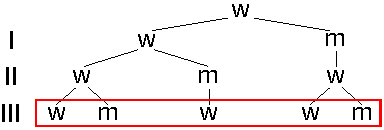
\includegraphics[scale=.6]{Layout.png}
	\caption{Aufteilung des Seitenlayouts mit viel Platz f\"{u}r Eure Randnotizen.}
	\label{fig:Seitenlayout}
\end{figure}


% Inhaltsverzeichnis
\tableofcontents
\newpage

\restoregeometry % nutze ab jetzt Notizenrand rechts 5.8.24 J.Hlawatsch

%\begin{ziele}
%	Hier stehen Ziele	
%\end{ziele}


\chapter{Denkanstöße}\label{Denk}

\begin{itemize}
\item
Warum sollen Menschen (Sch\"{u}ler) Physik erlernen?
\item
Kann man \say{Physik unterrichten} lernen?
\item
K\"{o}nnen Jungen Physik besser verstehen bzw.\ lernen?
\item
Warum sollen im Physikunterricht Experimente durchgef\"{u}hrt werden?
\item
Warum ist Physik das --- mit Abstand --- unbeliebteste Schulfach?
\item
Ist Physikdidaktik eine Wissenschaft?
\item
Warum geht von gro{\ss}en Denkleistungen gerade der Physik eine fast unvergleichliche Faszination aus?
\item
Kann man Physik nur mit Hilfe von Mathematik verstehen?
\item
Ist die Wissenschaft Physik Fluch oder Segen f\"{u}r die Menschheit?
\item
Ist ein Lehrplan f\"{u}r das Unterrichten notwendig?
\item
Sind angesichts von Computer, Beamern und ChatGPT  noch andere Medien sinnvoll?
\end{itemize}

\begin{uea}
	Beantworten Sie diese Fragen für sich und diskutieren Sie Ihre Gedanken mit Ihrem Nachbarn!
\end{uea}
\chapter{Begr\"{u}ndung von Physik in der Schule}\label{Begruendung}

Wie kann Physikunterricht gerechtfertigt ( = legitimiert) werden? \\
Ist es sinnvoll, Physik in der Schule zu unterrichten?

Unter welchen Gesichtspunkten ist diese Frage zu beantworten?
\begin{itemize}
	\item Aus der Sicht des Kindes?
	\item Aus der Sicht der Erziehenden?
	\item Aus der Sicht der Gesellschaft?
	\item Aus der Sicht der Wirtschaft?
\end{itemize}

\begin{enumerate}
	\item Kulturelle Identit\"{a}t

	\begin{enumerate}

		\item Lange Tradition einer Kultur in Europa, in Deutschland.

		\item Spezifisch naturwissenschaftliche Sichtweise:
		\begin{itemize}
			\item Naturwissenschaftliche Methode (Falsifikation von Hypothesen).
			\item Empirik (Experiment),
			\item Mathematisierung,
			\item Rationales Argumentieren,
			\item Exaktheit,
		\end{itemize}

		\item Entmythologisierung:
		\begin{itemize}
			\item \say{Die heilende Strahlkraft der Steine}
			\item Astronomie und Astrologie,
			\item Die teuflischen Handy-Strahlen.
		\end{itemize}

		\item Verantwortung f\"{u}r die Welt:
		\begin{itemize}
			\item Gestaltung der technischen Zivilisation
			\item Umwelterziehung: Kann ich anstelle einer Haushalts(Trocken-)Batterie auch ein Netzger\"{a}t verwenden?

		\end{itemize}


		\item Attribuierungen von Physik:
		\begin{itemize}
			\item Physik ist nicht nur die Technik-Hybris: Atombomben, Kraftwerke, Anonyme Apparate-Medizin,
			\item Ehrfurcht vor den Theorien der theoretisch-abstrakten Physik.
		\end{itemize}

	\end{enumerate}

	\item Lebensbew\"{a}ltigung

	\begin{enumerate}

		\item Handwerklich-technische Fertigkeiten, Berufsbildung
		\item Genaues Beobachten.

		\begin{itemize}
			\item In welcher Reihenfolge treten (welche) Farben im Regenbogen auf? In welcher Richtung ist der Bogen zu sehen?
		\end{itemize}


		\item Sprachliche Beschreibung:
		\begin{itemize}
			\item Stimmige Ausdrucksweisen: Der Strom flie{\ss}t, es liegt ein Spannung an,
			\item Bereicherung des Wortschatzes: El.\ Spannung, Druck, Temperatur, Verdampfen, Verdunsten, \dots
			\item Vertrautheit mit Einheiten.
		\end{itemize}

		\item Sicherheitsbewusstsein:
		\begin{itemize}
			\item Der F\"{o}hn in der Badewanne,
			\item Der Fotoapparat im Schwimmbad,
			\item Der Stuhl an der Wand,
		\end{itemize}

	\end{enumerate}

	\item Im Hinblick auf die Schule: Physik als \say{Methode}

	\begin{itemize}
		\item Farbe im Unterricht
		\item Spielerische Elemente,
		\item Handlungsorientierung,
		\item Soziale Lernziele: Gruppenexperiment,
		\item M\"{o}glichkeit zum Fach\"{u}bergriff:
		\begin{itemize}
			\item Mathematik: Gr\"{o}{\ss}enrechnen,
			\item Verkehrserziehung: Geschwindigkeit, Kr\"{a}fte, Fliehkr\"{a}fte, Bremswege.
		\end{itemize}

	\end{itemize}

	\item Weitere Gesichtspunkte:
	\begin{itemize}
		\item \"{A}sthetik,
		\item M\"{a}dchen und Physik,
		\item Entwicklung.
	\end{itemize}

\end{enumerate}
\chapter{Die Erkenntnis von Natur -- durch die Physik}\label{Erkenntnis}

{\bf Jeder} Mensch beobachtet unbefangen, unbewusst seine (Um-)Welt, die Natur, den Lebensalltag,
die technische Zivilisation. Er nimmt --- mit Hilfe der Sinnesorgane --- Ph\"{a}nomene wahr.

\begin{uea}
	Notieren Sie m\"{o}glichst viele Ph\"{a}nomene, die ein Schulkind wahrnimmt / kennt / mitvollzieht!
\end{uea}


\section{Physikalischer Erkenntnisweg}

Ein ,,Mensch mit physikalischer Zuneigung'' bem\"{u}ht sich,
\begin{itemize}
	\item diese Ph\"{a}nomene zu sammeln, zu erfassen,
	\item Zusammenh\"{a}nge zwischen diesen Ph\"{a}nomenen herzustellen,
	\item gemeinsame Erkl\"{a}rungen (Ursachen, Gesetze) f\"{u}r verschiedene Ph\"{a}nomene aufzufinden,
	\item die Erkl\"{a}rungen zu ordnen, zu systematisieren \quad und
	\item sie in exakter Form unter Benutzung rational-logischer Kategorien des menschlichen Geistes, oft in mathematischer Sprache, darzustellen.
\end{itemize}

Es entstehen dabei physikalische
\begin{itemize}
	\item Begriffe (Abstand, Zeit, Energie, Kraft, Drehimpuls)
	\item Modelle (el.\ Strom, Atommodell, Teilchenmodell)
	\item Teilgebiete (Mechanik, Optik, Elektrizit\"{a}tslehre, Optik, Atomphysik)
	\item Theorien (Newton'sche Mechanik, Maxwell'sche Elektrodynamik, Quantenmechanik, QED, GUT,\dots),
\end{itemize}

\mip
Da sich die Ph\"{a}nomene bei unbefangener Beobachtung teilweise sehr uneinheitlich, komplex,
unerkl\"{a}rlich darstellen, stellt der Physiker im Experiment gezielte Fragen an die Welt (Natur),
er achtet dabei auf
\begin{itemize}
	\item Beseitigung st\"{o}render Einfl\"{u}sse (Reibung, Ersch\"{u}tterungen, W\"{a}rmeverlust,\dots )
	\item Nachvollziehbarkeit (mit anderen Apparaturen, an beliebig anderem Ort, von anderen Personen)
	\item Wiederholbarkeit (zu beliebiger Zeit)
	\item Quantitative Erfassung (Messprozess)
	\item Genaue Dokumentation.
\end{itemize}

Es resultiert ein Wechselspiel aus
\begin{itemize}
	\item Experimentalphysik (empirische Methode) \quad und
	\item Theoretischer Physik (induktive und axiomatisch-deduktive Schlussfolgerungen).
\end{itemize}

Dieses Wechselspiel besteht in einer Abfolge von
\begin{itemize}
	\item Hypothesenbildung: Man gelangt zu Vermutungen \"{u}ber die Wirklichkeit durch intuitives --- deduktives Schlie{\ss}en auf der Grundlage schon bekannter Erkenntnisse.
	\item Verifikation an Beispielen bzw.\ Falsifikation
	\item Deutung innerhalb bestehender Theorien
	\item oder Erweiterung der bestehenden Theorien
\end{itemize}

\bip\bip
\section{Physik und Erziehung}
In welcher Form und mit welcher Intensit\"{a}t k\"{o}nnen Schulkinder an diesem Prozess teilnehmen?

Prinzipiell stehen sie einem Physiker nicht nach: Sie nehmen Ph\"{a}nomene wahr und entwickeln ihre eigenen Erkl\"{a}rungsmodelle. Sie bedienen sich dabei ihrer eigenen
\begin{itemize}
	\item entwicklungspsychologisch-altersgem\"{a}{\ss}en \quad und
	\item durch Lernen aus der Umwelt und sozialem Milieu
\end{itemize}
erworbenen Begriffswelt und Denkmuster.

\mip
Physik in der Schule soll nicht verstanden werden
\begin{itemize}
	\item als ein lediglich im Niveau herabgesetzter Wissensfundus,
	\item sondern als Prozess, an dem grunds\"{a}tzlich jeder Mensch und jedes Kind teilnehmen kann.
\end{itemize}

Das Streben nach physikalischer Erkenntnis ist Bestandteil der menschlichen Natur.

\mip
Die Aufgabe der ,,Physik in der Schule'' ist es, dieses Bestreben geeignet zu begleiten und
zu verfeinern. Dabei ist wichtig:
\begin{itemize}
	\item Kenntnis, wie Kinder ,,Physik vollziehen'',
	\item Kenntnis, wie Physiker ,,Physik vollziehen'',
	\item Kenntnis, wie der ,,Physik-Prozess des Physikers'' an den ,,Physik-Prozess im Kind'' angekoppelt werden kann.
\end{itemize}

Einige Grundthesen zur Physik im Unterricht:

\begin{enumerate}
	\item Der Mensch in allen Facetten seiner Gesamtpers\"{o}nlichkeit steht im Mittelpunkt jeden Unterrichts. So sind die Ehrfurcht vor dem Leben, die Achtung der Menschenrechte und das Bem\"{u}hen um eine Menschen-Bildung st\"{a}ndig neu zu verwirklichende Prinzipien in jeder Begegnung von Lehrer und Sch\"{u}ler. (Albert Schweitzer, Tausch/Tausch: Humanistische Pers\"{o}nlichkeitspsychologie)
	\item Die Physik umgibt heute eine Aura des Technizismus (vgl.\ das Negativ-Image infolge der Kernkraft- und Atombombendiskussion). Physik ist aber auch --- wenn nicht: vor allem --- eine Kulturleistung der Menschheit. (Vgl.\ die Hochachtung vor Nobelpreistr\"{a}gern).
	\item Physik als Wissen um Fakten und Methoden ist unverzichtbar in der Bew\"{a}ltigung des Lebens in unserer Gesellschaft (Industrie und Technik). Gleichwohl ist Physik \emph{nur ein} Bestandteil unseres Lebens.
	\item Charisma und Wissen um Didaktik sind zwei wesentliche Bestimmungsst\"{u}cke des Lehrerverhaltens.
	\item Beuys: Jeder Mensch ist ein K\"{u}nstler. Wagenschein (sinngem\"{a}{\ss}): Jeder Mensch ist ein Physiker: Aufgabe des Lehrers ist es, den Prozess der Physik im Sch\"{u}ler zu wecken und zu stimulieren.
\end{enumerate}

\chapter{Didaktische Modelle}\label{DidMod}

Dem Lernenden sind didaktische Modelle als abstrakte Grafiken aus Boxen und Pfeilen aus dem erziehungswissenschaftlichen Unterricht bekannt, in denen Pfeile von allem auf alles zeigen. In diesem Abschnitt soll die Bedeutung von Didaktischen Modellen als Grundlage der Unterrichtsgestaltung betont werden, denn die Prinzipien der Unterrichtsgestaltung greifen auf solche Modelle nat\"{u}rlich intrinsisch zur\"{u}ck. Siehe hierzu sp\"{a}ter Kapitel \ref{Entwurf}.

\mip

Ein allgemeindidaktisches Modell ist nach \textcite{JankMeyer} \begin{quote}{\glqq}\emph{ein erziehungswissenschaftliches Theoriegeb\"{a}ude zur Analyse und Modellierung didaktischen Handelns in schulischen und nichtschulischen Handlungszusammenh\"{a}ngen. \dots [es] stellt den Anspruch, theoretisch umfassend und praktisch folgenreich die Voraussetzungen, M\"{o}glichkeiten, Folgen und Grenzen des Lehrens und Lernens aufzukl\"{a}ren.}{\grqq} \end{quote} Insofern stellt ein didaktisches Modell einen eher formalen Rahmen dar, {\glqq}\dots innerhalb dessen didaktisches Handeln begr\"{u}ndet und strukturiert werden kann.{\grqq} Didaktische Modelle helfen dabei, Unterricht hinsichtlich seiner Ziele und Methoden diskutierbar und beurteilbar zu machen.

\mip

Ein aktuelles, oft zugrunde gelegtes didaktisches Modell, ist das  $\to$~\emph{Berliner Modell} (\cref{A_BerlinerModell}), das in den 1960er Jahren von Paul Heimann entwickelt wurde.  Das Berliner Modell bietet Lehrkr\"{a}ften ein klar strukturiertes Schema zur systematischen Planung und Reflexion des Unterrichts, das sowohl didaktische Entscheidungen als auch die spezifischen Lernbedingungen ber\"{u}cksichtigt. Es unterst\"{u}tzt die Lehrkraft dabei, den Unterricht zielgerichtet und den Bed\"{u}rfnissen der Lernenden entsprechend zu gestalten.

\mip

Das Modell basiert auf der Analyse und Gestaltung von sechs zentralen Elementen, die in zwei Kategorien unterteilt sind:

\begin{enumerate}

	\item Entscheidungsfelder

		\begin{itemize}

			\item Ziele: Welche Lernziele sollen erreicht werden? Hier wird festgelegt, welche Kenntnisse, F\"{a}higkeiten oder Haltungen die Sch\"{u}lerinnen und Sch\"{u}ler durch den Unterricht erwerben sollen.

			\item Inhalte: Welche Themen oder Inhalte werden behandelt? Die Auswahl und Anordnung der Unterrichtsinhalte m\"{u}ssen den Lernzielen entsprechen.

			\item Methoden: Welche Lehr- und Lernmethoden werden angewendet? Es wird festgelegt, wie die Inhalte vermittelt werden und welche didaktischen Prinzipien zum Einsatz kommen.

			\item Medien: Welche Materialien und Medien werden verwendet? Es geht um die Auswahl und den Einsatz von Unterrichtsmaterialien, die den Lernprozess unterst\"{u}tzen.

		\end{itemize}



	\item Bedingungsfelder

		\begin{itemize}

			\item	 Anthropogene Voraussetzungen: Welche Eigenschaften und F\"{a}higkeiten bringen die Lernenden mit? Dies umfasst Aspekte wie Vorkenntnisse, Lernmotivation und soziale Hintergr\"{u}nde der Sch\"{u}lerinnen und Sch\"{u}ler.

			\item Soziokulturelle Voraussetzungen: In welchem Kontext findet der Unterricht statt? Dazu z\"{a}hlen schulische Rahmenbedingungen, Klassengr\"{o}{\ss}e, Schulform, gesellschaftliche Erwartungen und Ressourcen.

		\end{itemize}

\end{enumerate}	



\pph{Wichtige Merkmale:}

\begin{itemize}

	\item Interdependenz der Felder: Die Entscheidungsfelder und Bedingungsfelder sind miteinander verkn\"{u}pft und beeinflussen sich gegenseitig. Eine \"{A}nderung in einem Feld kann Auswirkungen auf die anderen haben.

	\item Reflexionsm\"{o}glichkeit: Das Modell betont die Bedeutung der Reflexion und Anpassung des Unterrichts, basierend auf den Erfahrungen und Ergebnissen des Unterrichtsprozesses.

\end{itemize}	

Das $\to$\emph{Hamburger Modell} von Wolfgang Schulz aus den 1970er Jahren ist eine Weiterentwicklung des Berliner Modells. Es baut auf dem Berliner Modell auf, erweitert es aber um eine tiefere Reflexion der sozialen und ethischen Dimensionen des Unterrichts und legt mehr Wert auf die Erziehung und soziale Verantwortung innerhalb der Bildungsprozesse. Das Hamburger Modell



\begin{itemize}

	\item  legt st\"{a}rkeren Wert auf die kritische Reflexion von Lehr-Lern-Prozessen, einschlie{\ss}lich der ethischen und sozialen Implikationen,

	\item integriert die Frage nach sozialen und ethischen Werten st\"{a}rker in die Unterrichtsplanung und betont die soziale Interaktion und die gesellschaftliche Verantwortung des Unterrichts,

	\item versteht Didaktik umfassender als Erziehungswissenschaft, die sich nicht nur auf den Unterricht, sondern auch auf die Pers\"{o}nlichkeitsentwicklung der Lernenden richtet.

\end{itemize}



Wie wendet man ein solches Modell an, bzw. welche Bedeutung haben solche Modelle f\"{u}r die t\"{a}gliche Praxis der Lehrpersonen? Zur Beantwortung dieser Frage schaue man sich beispielsweise die Struktur des schriftlichen Unterrichtsentwurfes in $\to$Kapitel \ref{Entwurf} einmal genauer an. Die Bedingungs- und Entscheidungsfelder des Berliner Modells werden hier direkt beantwortet. Didaktische Modelle, wie hier konkret das Berliner und das Hamburger Modell, bilden somit das Fundament bei der Unterrichtsgestaltung.






\chapter{Merkmale guten Unterrichts}\label{GuterUnterricht}
Woher weiß man denn, ob Unterricht gut ist? Woher weiß man, ob man als Lehrender bzw. Lehrende keinen Schaden 
anrichtet? Es ist schwer,  eine allgemeing{\"u}ltige Beschreibung f{\"u}r guten Unterricht zu erstellen. Eine einfache Arbeitsdefinition k{\"o}nnte darin
bestehen, dass ein Unterricht dann gut ist, wenn eine gr{\"o}{\ss}tm{\"o}gliche Anzahl an Sch{\"u}lern vorher
festgelegte Ziele erreicht. Somit h{\"a}ngt nun die Beurteilung des Unterrichts auch von der Definition der Ziele ab und von den Methoden, wie diese Ziele erreicht werden!

\begin{beisp}
\begin{itemize}
\item
Ein sehr strenger Unterricht mit k{\"o}rperlicher Ma{\ss}regelung, wie zu Beginn des 20. Jahrhunderts durchaus {\"u}blich,
f{\"o}rdert das Auswendiglernen, behindert aber die freie Pers{\"o}nlichkeitsentwicklung.
\item
Freier Unterricht f{\"o}rdert die individuelle Pers{\"o}nlichkeitsentwicklung der Sch{\"u}ler, erbringt aber 
m{\"o}glicherweise weniger Spitzenleistungen als andere Unterrichtsformen.
\end{itemize}
\end{beisp}

Sp{\"a}ter werden wir das wichtige Wechselspiel von Unterrichtszielen, didaktischen Prinzipien, Unterrichtskonzepten und 
methodischer Umsetzung kennen lernen. F{\"u}r eine zusammenfassende Darstellung der Merkmale guten Unterrichts sei
hier auf den PIKO-Brief Nr. 4 verwiesen.

\bip\bip
\section{Die internationale Schulleistungsstudie PISA}
Das {\glqq}Programme for International Student Assessment{\grqq} (PISA) erfasst weltweit Sch{\"u}lerleistungen und vergleicht diese international. 
Initiator des Programms ist die OECD (Organisation f{\"u}r wirtschaftliche Zusammenarbeit und Entwicklung). Es werden 
 die Kompetenzen von 15-j{\"a}hrigen Jugendlichen beim Lesen, in der Mathematik
und den Naturwissenschaften erfasst. Sie wird alle drei Jahre erstellt. Die PISA-Studien werden als ein internationales 
Instrument angesehen, um alltags- und berufsrelevante Kenntnisse und F{\"a}higkeiten F{\"u}nfzehnj{\"a}hriger zu messen und vergleichbar zu machen.
PISA soll nicht nur eine Beschreibung des Ist-Zustandes liefern, sondern Verbesserungen ausl{\"o}sen. Zumindest  implizit wird der Anspruch 
erhoben, auf die nationalen Lehrpl{\"a}ne und Bildungsstandards zur{\"u}ckzuwirken.
\mip
Die Testaufgaben orientieren sich nicht an spezifischen Lehrpl\"{a}nen, sondern an Kompetenzen, die f{\"u}r den
Lernprozess und den Wissenserwerb wichtig sind. Naturwissenschaftliche Kompetenz beinhaltet, grundlegende 
naturwissenschaftliche Konzepte zu verstehen und mit naturwissenschaftlichen Denk- und Arbeitsweisen
vertraut zu sein.  

\bip\bip
\section{Basisdimensionen guten Unterrichts}

Es wurde,  der Versuch unternommen, u.a. und prominenterweise von Prof. Eckhard Klieme,\footnote{Eckhard Klieme (*1954), deutscher Bildungsforscher und Professor f{\"u}r Erziehungswissenschaft an der Johann Wolfgang Goethe-Universit{\"a}t Frankfurt am Main} aus der empirischen Unterrichtsforschung generische Grunddimensionen von Unterrichtsqualit{\"a}t zu entwickeln \autocite{Klieme}. Es lie{\ss}en sich drei Dimensionen voneinander abgrenzen:

\begin{itemize}
\item
Die erste Dimension \emph{Klassenf{\"u}hrung} fasst Skalen zur Regelklarheit, zu nachvollziehbaren Handlungsroutinen, zum Monitoring durch die Lehrkraft und zur St{\"o}rungspr{\"a}vention zusammen.

\item
Die zweite Dimension \emph{Sch{\"u}lerorientierung} f{\"u}hrt Skalen wie die Sensitivit{\"a}t f{\"u}r individuelle Bed{\"u}rfnisse, Unterst{\"u}tzung durch die Lehrkraft und die Abwesenheit von Leistungsdruck zusammen. In anderen Publikationen wird das als \emph{sch{\"u}lerorientiertes Unterrichtsklima} bzw. \emph{konstruktive Unterst{\"u}tzung} bezeichnet.

\item
Die dritte Dimension fasst unter dem Begriff \emph{kognitive Aktivierung} die Verwendung von Erkl{\"a}rungen und Aufgabenstellungen zusammen, die die SuS herausfordern, an vorhandenes Wissen anzukn{\"u}pfen und sich durch eigenst{\"a}ndiges Nachdenken neues Wissen zu erschlie{\ss}en.
\end{itemize}

Diese Basisdimensionen sind mittlerweile gut etabliert. Sie stimmen gut mit den international anerkannten Dimensionen {\glqq}Organisational Support{\grqq}, {\glqq}Emotional Support{\grqq} und  {\glqq}Instructional Support{\grqq} {\"u}berein.

\bip\bip
\section{Die IPN Interessenstudie Physik ({\glqq}Kieler{\grqq} Interessenstudie)}
Am Leibniz-Institut f{\"u}r die P{\"a}dagogik der Naturwissenschaften und Mathematik (IPN) in Kiel wurde eine Videostudie zur Beschreibung und Erkl{\"a}rung von Lehr-Lern-Prozessen im Physikunterricht erstellt. Die Ergebnisse des sechsj{\"a}hrigen Forschungsprojekts zeigen zum einen, wie einheitlich Physikunterricht in Deutschland hinsichtlich der Klassenorganisation, der Zielorientierung, der Lernbegleitung, der Fehlerkultur und der Experimente abl{\"a}uft. Zum anderen lassen die Analysen differentielle Effekte des Unterrichts auf Lernentwicklungen bei Sch{\"u}lerinnen und Sch{\"u}lern erkennen.
\mip
Wesentliche Ergebnisse lassen sich wie folgt zusammenfassen:
\begin{itemize}
\item
Kein Unterricht ist gleichwertig zu betrachten, jeder Unterricht hat St{\"a}rken und Schw{\"a}chen. Jeder Unterricht ist indviduell, jede Lehrkraft hat eigene {\glqq}Handschrift{\grqq}.
\item
 Experimente haben grosse Bedeutung, ca 70\% des Unterrichts werden vom Experiment bestimmt. Das Sch{\"u}lerexperiment ist zeitaufw{\"a}ndiger als das Demonstrationsexperiment. Es gibt signifikante Unterschiede zwischen den Lehrkr{\"a}ften. Sch{\"u}ler sind im Durchschnitt nur wenig bei Planung, Durchf{\"u}hrung, Auswertung von Experimenten beteiligt.
 \item
Unterricht ist typischerweise lehrerzentriert. Nur 17\% der Unterrichtszeit entfallen auf Sch{\"u}lerarbeitsphasen. Dominant ist das eng gef{\"u}hrte Klassengespr{\"a}ch im Stile des fragend-entwickelnden Verfahrens.
\item
Der Unterricht bietet nur wenig Gelegenheit f{\"u}r die aktive und eigenst{\"a}ndige Auseinandersetzung mit dem Stoff.
\item
Unterricht {\"u}ber {\glqq}klassische{\grqq} Inhalte dominiert; naturwissenschaftliche Denk- und Arbeitsweisen werden nur selten angesprochen.
\item
Viele Lehrkr{\"a}fte haben keine explizite Vorstellung,  wie Lernen funktioniert und welche Rolle sie beim Lernen einnehmen sollten. Z.~B. Rolle von Sch{\"u}lervorstellungen beim Lernen von Physik und zur F{\"o}rderung des Interesses kaum bekannt.
\end{itemize}


\bip\bip
\section{Die Hattie-Studie}
Der neuseel{\"a}ndische Bildungsforscher John Hattie erstellte eine international beachtete Studie zum Themenfeld {\glqq}Schulunterricht{\grqq}, 
welche er im Jahre 2009 in seinem Buch \emph{Visible learning} vorstellte. In der Studie wurden die Ergebnisse von hunderten Metaanalysen zusammengef{\"u}rt,
welche aus vielz{\"a}ligen Lernstandserhebungen gewonnen wurden. Hattie stellte Einflussfaktoren auf Sch{\"u}lerleistungen und erfolgreiches Lernen zusammen. 
\mip
Zur Beurteilung von Einflussfaktoren auf den schulischen Lernerfolg ermittelte Hattie eine Effektst{\"a}rke, mit deren Hilfe er den Effekt einer 
bestimmten Ma{\ss}nahme auf den Lernerfolg bewertet. Hattie konnte somit darlegen, dass es weiterhin stark auf die Lehrperson ankomme, 
ob Sch{\"u}ler in der Schule erfolgreich sind.
\mip

Einige Beispiele:
\begin{itemize}
\item
{\emph{Sch{\"a}dlich f{\"u}r den Lernerfolg:}} Umzug, Krankheit, Fernsehen, Alleinerziehende Eltern, Sitzenbleiben, Sommerferien.
\item
{\emph{Was hilft nicht und schadet nicht:}} Offener Unterricht, Leistungsgruppierung, Interne Differenzierung, Web-basiertes Lernen, team-teaching.
\item
{\emph{Was hilft ein wenig:}} Reduzierung der Klassengr{\"o}{\ss}e, individualisiertes Lernen, Integration und Inklusion, Hausaufgaben, entdeckendes Lernen, induktives Unterrichten, regelm{\"a}{\ss}ige Leistungskontrollen, Zusatzangebote f{\"u}r Leistungsstarke.
\item
{\emph{Was hilft schon mehr:}} Angstreduktion, kooperatives Lernne, Kleingruppenlernen, peer tutoring, direkte Instruktion.
\item
{\emph{Was hilft richtig viel:}} Regelm{\"a}{\ss}ige Tests mit Feedback, metakognitive Strategien, Lehrkraft-Sch{\"u}ler-Verh{\"a}ltnis, Klarheit der Instruktion, Micro-Teaching, Akzelerationsprogramme, Formatives Assessment. 
\end{itemize}




%----------------------------------------eingefuegt Axel Enders 26.10.2023-----------------------------------------------------------------------------------------
\newpage
\chapter{Bildungsstandards und die KmK}\label{KmK}
Die Kultusministerkonferenz (KmK) hat beschlossen,\footnote{KMK $\textrm{--}$ St{\"a}ndige Konferenz der Kultusminister in der Bundesrepublik Deutschland (2004): Bildungsstandards im Fach Pysik f{\"u}r den Mittleren Schulabschluss. Beschluss vom 16.12.2004. Bonn: KMK.} Bildungsstandards zu erarbeiten mit dem Ziel, die Einheitlichkeit und Vergleichbarkeit von Zeugnissen und Abschl{\"u}ssen zwischen den Bundesl{\"a}ndern zu vereinbaren und dadurch ein H{\"o}chstma{\ss} an Mobilit{\"a}t von Fachkr{\"a}ften innerhalb der Bundesrepublik zu erreichen und  zur Gleichwertigkeit der Lebensverh{\"a}ltnisse in ganz Deutschland beizutragen. Die Bundesl{\"a}nder haben sich verpflichtet, diese Standards zu implementieren und anzuwenden. Diese (m{\"u}hsam errungenen) Bildungsstandards werden allgemein als nationale Kompetenzziele angesehen und sollen als Messlatte f{\"u}r den Erfolg des Schulunterrichts, u.a. im Fach Physik, dienen. 
\mip
Mit dem Erwerb des mittleren Schulabschlusses verf{\"u}gen die SuS {\"u}ber naturwissenschaftliche \emph{Kompetenzen} im Allgemeinen, und {\"u}ber physikalische Kompetenzen im Besonderen. 
\mip
\leftskip=0.5cm \rightskip=0.5cm {\emph{{\textbf{Definition von Kompetenzen}} nach Weinert:\footnote{Weinert, F. E., Vergleichende Leistungsmessung in Schulen $\textrm{--}$ eine umstrittene Selbstverst{\"a}ndlichkeit, in: Weinert, F. E. (Hrsg.), Leistungsmessungen in Schulen, 2001} die bei Individuen verf{\"u}gbaren oder durch sie erlernbaren kognitiven F{\"a}higkeiten und Fertigkeiten, um bestimmte Probleme zu 
l{\"o}sen, sowie die damit verbundenen motivationalen, volitionalen und sozialen Bereitschaften und F{\"a}higkeiten, um die Probleml{\"o}sungen in variablen Situationen erfolgreich und verantwortungsvoll nutzen zu k{\"o}nnen.}} 
\mip
%  \tabto{12em} \hangindent=4.62cm
\leftskip=0cm \rightskip=0cm Die in den folgenden vier Kompetenzbereichen festgelegten Standards beschreiben die notwendige physikalische Grundbildung. Zu jedem Kompetenzbereich sind drei Anforderungsbereiche  (= Merkmale von Aufgaben, die verschiedene Schwierigkeitsgrade innerhalb ein und derselben Kompetenz abbilden), \textbf{I}, \textbf{II}, \textbf{III}, angegeben. 
\mip
{\textbf{Fachwissen}} \tabto{7em} \hangindent=2.7cm Physikalisches Fachwissen, wie es durch die vier Basiskonzepte (Materie, Wechselwirkungen,System, Energie) charakterisiert wird, beinhaltet Wissen {\"u}ber Ph{\"a}nomene, Begriffe, Bilder, Modelle und deren G{\"u}ltigkeitsbereiche sowie {\"u}ber funktionale Zusammenh{\"a}nge und Strukturen. Als strukturierter Wissensbestand bildet das Fachwissen die Basis zur Bearbeitung physikalischer Probleme und Aufgaben. \\ \emph{\textbf{I} Wissen wiedergeben; \textbf{II} Wissen anwenden; \textbf{III} Wissen transferieren und verkn{\"u}pfen}
\mip
{\textbf{Erkenntnisgewinnung}} \tabto{12em} \hangindent=2.7cm Physikalische Erkenntnisgewinnung ist ein Prozess, der durch die T\"{a}tigkeiten \emph{Wahrnehmen}, \emph{Ordnen}, \emph{Erkl{\"a}ren bzw. Pr{\"u}fen} sowie \emph{Modelle bilden} beschrieben werden kann. \\ \emph{\textbf{I} Fachmethoden beschreiben; \textbf{II} Fachmethoden nutzen; \textbf{III} Fachmethoden problembezogen ausw{\"a}hlen und anwenden}
\mip
{\textbf{Kommunikation}} \tabto{9em} \hangindent=2.7cm Informationen sach- und fachbezogen erschlie{\ss}en und austauschen. Dazu geh{\"o}ren das angemessene Verstehen von Fachtexten, Graphiken und Tabellen, der Umgang mit Informationsmedien sowie das Dokumentieren von gewonnenem Wissens. Zur Kommunikation sind die Sprech- und Schreibf{\"a}higkeit in der Alltags- und der Fachsprache, das Beherrschen der Diskussion und Techniken der Pr{\"a}sentation erforderlich. \\ \emph{\textbf{I} Mit vorgegebenen Darstellungsformen arbeiten; \textbf{II} Geeignete Darstellungsformen nutzen; \textbf{III} Darstellungsformen selbst{\"a}ndig ausw{\"a}hlen und nutzen}
\mip
{\textbf{Bewertung}} \tabto{7em} \hangindent=2.7cm Physikalische Sachverhalte in verschiedenen Kontexten erkennen und bewerten. Dazu geh{\"o}ren das Heranziehen physikalischer Denkmethoden und Erkenntnisse zur Erl{\"a}uterung, zum Verst{\"a}ndnis und zur Bewertung physikalisch-technischer und gesellschaftlicher Entscheidungen, sowie die Kenntnis der Grenzen naturwissenschaftlicher Sichtweisen. \\ \emph{\textbf{I}  Vorgegebene Bewertungen nachvollziehen; \textbf{II} Vorgegebene Bewertungen beurteilen und kommentieren; \textbf{III} Eigene Bewertungen vornehmen}




\chapter{Lernziele}\label{Lernziel}\label{Ziele}

%\begin{ziele}
%	Am Ende dieses Kapitels können Sie...
%	\begin{itemize}
%		\item erläutern, was Lernziele sind und welche Funktionen sie haben.
%		\item zu einem gegebenen Themengebiet Lernziele entwickeln.
%		\item Lernziele entsprechend der Taxonomie von Anderson und Krathwohl einordnen.
%		\item Aufgaben hinsichtlich der Kompetenzbereiche der KmK klassifizieren.
%	\end{itemize}	
%\end{ziele}

Als Vorüberlegung zu diesem Kapitel beschäftigen Sie sich bitte mit folgender
\begin{uea}
	Versetzen Sie sich zurück in Ihre Schulzeit und beantworten Sie folgende Fragen:
	\begin{enumerate}
		\item Was wurde im Physikunterricht \emph{gelehrt}?
		\item Was haben Sie im Physikunterricht \emph{gelernt}?
		\item Was haben Sie nach Besuch des Physikunterrichts \emph{gekonnt}?
	\end{enumerate}
	Tauschen Sie sich anschließend mit einem Partner aus.	
\end{uea}

Möglicherweise sind Ihre Antworten auf die Fragen 1, 2 und 3 nicht kongruent. Die lerntheoretische Strömung des \emph{Konstruktivismus} ($\to$ \cref{Konstruktivismus}) hat dafür eine einfache Erklärung: Etwas zu lernen erfordert eine aktive Konstruktion des Lerninhalts und damit verbundener Kompetenzen durch den Lernenden. Lehr- und Lernziele müssen also nicht übereinstimmen (siehe auch $\to$ \cref{EVA}).

\section{Lernen ordnen: Zum Begriff des Lernziels}
Jedes planm\"{a}{\ss}ige Handeln erfordert eine Zielsetzung:
So hat sich in der lerntheoretisch orientierten Unterrichtsforschung im Laufe der Zeit der Gedanke
der Zielformulierung durchgesetzt.
\mip
Der Begriff {\bf Lernziel} deutet dabei auf ein Endverhalten
der Sch\"{u}ler hin ($\to$ Operationalisierung). Es geht zun\"{a}chst weniger um die Art oder die Methodik
des Lernprozesses.
\mip
Ein Weg kann klarer ausgew\"{a}hlt und leichter beschritten werden,
wenn das Ziel bekannt ist.

\begin{itemize}
	\item Lernziele bilden f\"{u}r den Lehrenden den entscheidenden Rahmen f\"{u}r die
	Unterrichtsplanung und -umsetzung.
	\item Lernziele geben den Lernenden eine Orientierung über die von ihnen regelmäßig erwarteten Handlungsmuster und Lernerfolge.
	\item In Lernzielen werden die Erwartungen einer Gesellschaft
	(einschlie{\ss}lich Wirtschaft, Verb\"{a}nde, Kirchen, Hochschulen) an
	die Institution ,,Schule'' formuliert.
	\item Traditionen, neue Entwicklungen, Weltanschauungen oder
	Ideologien schlagen sich in den Lernzielen nieder.
	Beispiele: NewMaths, Umweltbewegung, Europa.
	\item
	Sie spiegeln deshalb den st\"{a}ndigen gesellschaftlichen
	Wechselprozess aus Bewahrung und Ver\"{a}nderung wieder.
%	\item
%	Im Begriff ,,Lernziel'' begegnen sich zwei grundlegende
%	Dimensionen von Unterricht:
%	
%	\begin{itemize}
%		\item
%		Auftrag zur Bildung der Pers\"{o}nlichkeit
%		(Anthropologische oder personale Dimension)
%		\item
%		Vermittlung fach(wissenschaft)licher Inhalte (Sachliche
%		oder inhaltliche Dimension)
%	\end{itemize}
\end{itemize}

\section{Funktionen von Lernzielen}
\begin{itemize}
	\item Lernziele sind -- gemeinsam mit den Lernvoraussetzungen -- gedanklicher Ausgangspunkt jeder Unterrichtsplanung ($\to$ \cref{Entwurf}). Schematisch dargestellt: \begin{equation*}
		\text{Lernvoraussetzungen} \longrightarrow \text{Unterrichtliches Handeln} \longrightarrow \text{Lernziele.}
	\end{equation*}
	\item Lernziele ermöglichen die Evaluation und Reflexion von Unterricht. Die Erreichung der Lernziele durch die Lernenden ist hierbei das Gütekriterium (und nicht etwa die vollständige und fachlich korrekte Darstellung durch die Lehrkraft).
	\item Lernziele stellen in den Mittelpunkt den Lernprozess der
	Sch\"{u}ler und nicht die Fachinhalte (Lerninhalte) oder
	die Unterrichtsmethodik (Lehrziele).
	\item
	Lernziele stellen ein Instrument f\"{u}r die Diskussion \"{u}ber
	schulische Erziehung und Unterricht bereit und bilden
	daher eine M\"{o}glichkeit zur Verst\"{a}ndigung von Lehrern,
	Sch\"{u}lern, Eltern, Didaktikern, Bildungspolitikern
	(Beispiel: Weltanschaulicher Unterricht, Sexualkunde).
	\item
	Der normative Charakter von Lernzielen erm\"{o}glicht es, den
	gesellschaftlichen Konsens \"{u}ber die Schule in den Unterricht zu
	transportieren.
	
	\mip
	Lehrpl\"{a}ne (in Bayern) werden vom Kultusministerium verordnet,
	und im Amtsblatt ver\"{o}ffentlicht. Die derzeit gültige Version ist der LehrplanPlus, der unter \url{lehrplanplus.bayern.de} abrufbar ist.
\end{itemize}

\section{Lernzielebenen}

Lernziele lassen sich hierarchisch danach ordnen, über welche zeitliche Tragweite sie für die Unterrichtsplanung relevant sind. Eine ausführliche Darstellung der Lernzielebenen nach Westphalen (1979) findet sich bei \textcite{KircherGirwidzHaussler1} auf den Seiten 90 ff. Hier eine kurze Übersicht:

\begin{enumerate}
	\item \textbf{Leitziele:} Oberste, fächerübergreifende Ebene pädagogischer Aufgaben und Absichten, siehe $\to$ \href{https://www.gesetze-bayern.de/Content/Document/BayVerf-131}{Art. 131 BV}, $\to$ \href{https://www.gesetze-bayern.de/Content/Document/BayEUG-1}{Art. 1 BayEUG}.
	\begin{beisp}
		Studierf\"{a}higkeit, Berufsf\"{a}higkeit, Allgemeinbildung, Bew\"{a}ltigung der Lebenswelt, gesellschaftliche Verantwortung.
	\end{beisp}

	\item \textbf{Richtziele:} Genauere, teilweise fachspezifische Ausformulierungen der Leitziele, siehe $\to$ Fachprofil des Fachs Physik im LehrplanPlus.
	\begin{beisp}
		Förderung des Verständnisses naturwissenschaftlicher Methoden und Denkweisen, Entwicklung von Problemlösungsfähigkeiten, Verständnis der Rolle der Physik in der Gesellschaft.
	\end{beisp}


	\item \textbf{Grobziele} beschreiben eindeutig, aber nicht im Detail, die angestrebten Lernergebnisse innerhalb eines Faches. Denken Sie bei einem Grobziel an ein Lernziel mehrerer Unterrichtseinheiten. Sie finden diese durch die Gesamtschau des Fachlehrplans.

	\begin{beisp}
		aus dem LPP Ph9: Verständnis der Energieerhaltung, Anwendung physikalischer Modelle, Bewertung gesellschaftlicher Auswirkungen
	\end{beisp}

	\item \textbf{Feinziele (auch Unterrichtsziele, Teilziele)} differenzieren den Unterricht in kleinste Einzelziele. Sie erhalten sie aus einzelnen, im Lehrplan angegebenen Kompetenzerwartungen. Ggf. müssen Sie diese noch konkretisieren.

	\begin{beisp}
		aus dem LPP Ph9: Die Schülerinnen und Schüler nutzen das Prinzip der Energieerhaltung, um bei Energieumwandlungen mechanische Energieformen quantitativ zu bilanzieren und Größen zu berechnen.
	\end{beisp}
\end{enumerate}

Diese Unterteilung ist nicht vollständig trennscharf. Für Ihre Unterrichtsvorbereitung ($\to$ \cref{Entwurf}) sind vor allem Grob- und Feinziele relevant, wobei Sie Leit- und Richtziele im Hinterkopf behalten. Im schriftlichen Unterrichtsentwurf geben Sie die Ebenen 3 und 4 an.

\section{Lernzieltaxonomien und Operationalisierung}

\begin{table}[bh] \tiny
\begin{tabular}{l|l|l|l|l|l|l}
 \multirow{2}{*}{Dimension \NL des Wissens}                 & \multicolumn{6}{c}{Dimension kognitiver Prozesse}                                        \\
                  & 1. Erinnern & 2. Verstehen & 3. Anwenden & 4. Analysieren & 5. Beurteilen & 6. Erschaffen \\ \hline
 A. Faktenwissen  &             &              &             &                &              &               \\ \hline
 B. Konzeptwissen &             &              &             &                &              &               \\ \hline
 C. Prozesswissen &             &              &             &                &              &               \\ \hline
 D. Metakognition &             &              &             &                &              &              
\end{tabular}\caption{Darstellung der Taxonomie nach Anderson und \textcite{Krathwohl}.}\label{tab:krathwohl}
\end{table}

Lernziele lassen sich nach verschiedenen Dimensionen des Gesamtspektrums menschlicher Verhaltensweisen einordnen. Die darauf aufbauenden Klassifizierungen hei{\ss}en Taxonomien (Einordnung, vgl.\ z.B.\ Biologie). Die bekannteste ist wohl die Taxonomie nach \textcite{Bloom}. Hier dargestellt wird die darauf aufbauende Taxonomie nach Anderson und \textcite{Krathwohl}.

Die Taxonomie weist zwei Dimensionen auf, die \emph{Dimension des Wissens} und die \emph{Dimension kognitiver Prozesse}, da die kognitiven Prozesse der Auseinandersetzung mit dem Lerngegenstand auf jeder Ebene auf Wissen im Hinblick auf den Lerngegenstand zurückgreifen.

\subsection{Zur Dimension des Wissens}
\begin{enumerate}[label=\Alph*.]
	\item \textbf{Faktenwissen:} Die grundlegenden Elemente, die Schüler wissen müssen, um Probleme zu lösen.
	\item \textbf{Konzeptwissen:} Die Beziehungen zwischen den grundlegenden Elementen innerhalb einer größeren Struktur, durch die sie gemeinsam funktionieren.
	\item \textbf{Prozesswissen:} Wie man etwas macht, Forschungsmethoden, und Kriterien zur Auswahl von Techniken und Methoden der Problemlösung.
	\item \textbf{Metakognitives Wissen:} Wissen um sowie über die eigene Kognition.
\end{enumerate}

\subsection{Zur Dimension koginitiver Prozesse}
\begin{enumerate}
	\item \textbf{Erinnern:} Relevantes Wissen aus dem Langzeitgedächtnis abrufen.
	\item \textbf{Verstehen:} Die Bedeutung von Lerninformationen bestimmen und mündlich, schriftlich, graphisch darstellen.
	\item \textbf{Anwenden:} Ein Verfahren in einer bestimmten Situation anwenden.
	\item \textbf{Analysieren:} Material in seine Bestandteile zerlegen und deren wechselseitige Beziehung und Zusammensetzung zum Ganzen erörtern.
	\item \textbf{Beurteilen:} Werturteile auf Grundlage von Kriterien und Standards fällen.
	\item \textbf{Erschaffen:} Elemente zu einem neuen Ganzen zusammensetzen oder ein Produkt entwickeln.
\end{enumerate}

\begin{uea}
	Ordnen Sie folgende Lernziele den Bereichen in \cref{tab:krathwohl} zu.
	\begin{enumerate}[label=\alph*.]
		\item Die Schüler können den Ablauf eines Experiments in seine einzelnen Schritte zerlegen und die Bedeutung jedes Schrittes im Kontext der Energieerhaltung erläutern.
		\item Die Schüler können mithilfe des Energieerhaltungssatzes erklären, wie Energie in geschlossenen Systemen erhalten bleibt.
		\item Die Schüler können ihre eigenen Denkprozesse beim Lösen von Aufgaben zur Energieerhaltung reflektieren und geeignete Strategien entwickeln, um Probleme effizienter zu lösen.
		\item Die Schüler können das Prinzip der Energieerhaltung anwenden, um in mechanischen Prozessen Energieumwandlungen zu berechnen.
		\item Die Schüler können die grundlegenden Konzepte der Energieerhaltung und die verschiedenen Energieformen (z. B. kinetische Energie, potenzielle Energie) aufzählen.
	\end{enumerate}
	Entwerfen Sie dann drei weitere, eigene Lernziele zu Bereichen, die noch nicht belegt sind.
	
	\flushright\rotatebox{180}{\tiny Lösung: C4, A2, D6, B3, A1}
\end{uea}

\subsection{Operationalisierung}
Vielleicht ist Ihnen aufgefallen, dass die Beispiele in der vorigen Übungsaufgabe alle eine bestimmte Struktur besitzen: Sie beginnen mit \emph{Die Schüler können}, gefolgt von einem \emph{Operatorverb} wie erläutern, erklären, reflektieren, entwickeln, anwenden, aufzählen.

\mip
Auf diese Weise formulierte Lernziele nennt man \textbf{Operationalisierte Lernziele}. Sie geben das gewünschte Endverhalten der Schüler an und machen die in der Unterrichtsplanung angegebenen Lernziele somit abprüfbar. Sie können aus dem Lernziel direkt Aktivitäten und Aufgaben ableiten. Auch Lernziele im LehrplanPlus werden operationalisiert angegeben, wobei zusätzlich zu den erworbenen Kompetenzen Inhalte angegeben werden.

\mip
Ein enges Verständnis von Operationalisierten Lernzielen findet man bei Mager und \textcite{Gagne}. Hier darf das Lernziel keinen Interpretations\-spielraum mehr zulassen. Dies wird bewerkstelligt durch folgende Bedingungen:
\begin{enumerate}
	\item	Benennung des Endverhaltens, das direkt beobachtbar sein muss ($\to$ Behaviorismus).
	\item	Eindeutige Bezeichnung des Gegenstandes, auf den sich Lernziel bezieht.
	\item	Beschreibung der Rahmenbedingungen, Voraussetzungen, Hilfsmittel (z.B.\ Formelsammlung, Taschenrechner).
	\item	Angabe eines Beurteilungsma{\ss}stabes  f\"{u}r das als ausreichend 	geltendes Verhalten.
\end{enumerate} 
Zentral ist die Verwendung von Operatorverben, die auf Lernzielebenen referieren ($\to$ Verbliste im Anhang).

\begin{beisp}
	\textbf{Klassisch (veraltet):} \\ 
	Der Sch\"{u}ler soll Aufbau und Wirkungsprinzipien eines
	Elektromotors verstehen.
	
	\mip
	\textbf{Operationalisiert (üblich):} \\
	Der Sch\"{u}ler soll das Modell eines Elektromotors aufbauen k\"{o}nnen,
	seine wichtigsten Teile benennen und ihre Funktion erkl\"{a}ren k\"{o}nnen.
	
	\mip
	\textbf{In Reinform (fast zuviel, aber als Übung und für Unterrichts- und Prüfungsvorbereitung nützlich):} \\
	Der Sch\"{u}ler soll das Leybold-Modell eines Elektromotors
		innerhalb von 10 Minuten aufbauen und verschalten k\"{o}nnen, er
		soll weiter die Begriffe ,,Stator, Rotor, Kommutator'' im
		Modell zuordnen k\"{o}nnen und die Funktion jedes dieser Bauteile
		in zwei S\"{a}tzen beschreiben k\"{o}nnen, (wobei zwei Fehler erlaubt
		sind).
\end{beisp}

%----------------------------------------eingefuegt Axel Enders 26.10.2023----------------------------------------------------------------------------------------- vormals Kapitel 6

\section{Bildungsstandards und die KmK}\label{KmK}
Die Kultusministerkonferenz (KmK) hat beschlossen, Bildungsstandards zu erarbeiten mit dem Ziel, die Einheitlichkeit und Vergleichbarkeit von Zeugnissen und Abschl{\"u}ssen zwischen den Bundesl{\"a}ndern zu vereinbaren und dadurch ein H{\"o}chstma{\ss} an Mobilit{\"a}t von Fachkr{\"a}ften innerhalb der Bundesrepublik zu erreichen und  zur Gleichwertigkeit der Lebensverh{\"a}ltnisse in ganz Deutschland beizutragen \autocite{KMK}. Die Bundesl{\"a}nder haben sich verpflichtet, diese Standards zu implementieren und anzuwenden. Diese (m{\"u}hsam errungenen) Bildungsstandards werden allgemein als nationale Kompetenzziele angesehen und sollen als Messlatte f{\"u}r den Erfolg des Schulunterrichts, u.a. im Fach Physik, dienen. 
\mip
Mit dem Erwerb des mittleren Schulabschlusses verf{\"u}gen die SuS {\"u}ber naturwissenschaftliche \emph{Kompetenzen} im Allgemeinen, und {\"u}ber physikalische Kompetenzen im Besonderen. 
\mip
\leftskip=0.5cm \rightskip=0.5cm {\emph{{\textbf{Definition von Kompetenzen}} nach \textcite{Weinert}: die bei Individuen verf{\"u}gbaren oder durch sie erlernbaren kognitiven F{\"a}higkeiten und Fertigkeiten, um bestimmte Probleme zu 
l{\"o}sen, sowie die damit verbundenen motivationalen, volitionalen und sozialen Bereitschaften und F{\"a}higkeiten, um die Probleml{\"o}sungen in variablen Situationen erfolgreich und verantwortungsvoll nutzen zu k{\"o}nnen.}} 
\mip
%  \tabto{12em} \hangindent=4.62cm
\leftskip=0cm \rightskip=0cm Die in den folgenden vier Kompetenzbereichen festgelegten Standards beschreiben die notwendige physikalische Grundbildung. Zu jedem Kompetenzbereich sind drei Anforderungsbereiche  (= Merkmale von Aufgaben, die verschiedene Schwierigkeitsgrade innerhalb ein und derselben Kompetenz abbilden), \textbf{I}, \textbf{II}, \textbf{III}, angegeben. 
\mip
{\textbf{Fachwissen}} \tabto{7em} \hangindent=2.7cm Physikalisches Fachwissen, wie es durch die vier Basiskonzepte (Materie, Wechselwirkungen, System, Energie) charakterisiert wird, beinhaltet Wissen {\"u}ber Ph{\"a}nomene, Begriffe, Bilder, Modelle und deren G{\"u}ltigkeitsbereiche sowie {\"u}ber funktionale Zusammenh{\"a}nge und Strukturen. Als strukturierter Wissensbestand bildet das Fachwissen die Basis zur Bearbeitung physikalischer Probleme und Aufgaben. \\ \emph{\textbf{I} Wissen wiedergeben; \textbf{II} Wissen anwenden; \textbf{III} Wissen transferieren und verkn{\"u}pfen}
\mip
{\textbf{Erkenntnisgewinnung}} \tabto{12em} \hangindent=2.7cm Physikalische Erkenntnisgewinnung ist ein Prozess, der durch die T\"{a}tigkeiten \emph{Wahrnehmen}, \emph{Ordnen}, \emph{Erkl{\"a}ren bzw. Pr{\"u}fen} sowie \emph{Modelle bilden} beschrieben werden kann. \\ \emph{\textbf{I} Fachmethoden beschreiben; \textbf{II} Fachmethoden nutzen; \textbf{III} Fachmethoden problembezogen ausw{\"a}hlen und anwenden}
\mip
{\textbf{Kommunikation}} \tabto{9em} \hangindent=2.7cm Informationen sach- und fachbezogen erschlie{\ss}en und austauschen. Dazu geh{\"o}ren das angemessene Verstehen von Fachtexten, Graphiken und Tabellen, der Umgang mit Informationsmedien sowie das Dokumentieren von gewonnenem Wissens. Zur Kommunikation sind die Sprech- und Schreibf{\"a}higkeit in der Alltags- und der Fachsprache, das Beherrschen der Diskussion und Techniken der Pr{\"a}sentation erforderlich. \\ \emph{\textbf{I} Mit vorgegebenen Darstellungsformen arbeiten; \textbf{II} Geeignete Darstellungsformen nutzen; \textbf{III} Darstellungsformen selbst{\"a}ndig ausw{\"a}hlen und nutzen}
\mip
{\textbf{Bewertung}} \tabto{7em} \hangindent=2.7cm Physikalische Sachverhalte in verschiedenen Kontexten erkennen und bewerten. Dazu geh{\"o}ren das Heranziehen physikalischer Denkmethoden und Erkenntnisse zur Erl{\"a}uterung, zum Verst{\"a}ndnis und zur Bewertung physikalisch-technischer und gesellschaftlicher Entscheidungen, sowie die Kenntnis der Grenzen naturwissenschaftlicher Sichtweisen. \\ \emph{\textbf{I}  Vorgegebene Bewertungen nachvollziehen; \textbf{II} Vorgegebene Bewertungen beurteilen und kommentieren; \textbf{III} Eigene Bewertungen vornehmen}





\chapter{Sch{\"u}lervorstellungen und Konzeptwechsel}\label{Schuelervorstellungen}


\section{Konstruktivismus}\label{Konstruktivismus}

Der Konstruktivismus ist eine lerntheoretische Perspektive, die das Lernen nicht als eine Folge des Lehrens beschreibt, sondern als eigenst"{a}ndige Konstruktionsleistung des Lernenden. Lernen wird als individueller, aktiver Prozess verstanden, bei dem neue Informationen auf Basis von Vorerfahrungen und bereits vorhandenen Wissensstrukturen interpretiert und integriert werden. Somit betont der konstruktivistische Ansatz  die aktive Rolle des Lernenden im Lernprozess. Insbesondere die Extremform des Konstruktivismus, der \emph{radikale} Konstruktivismus, bewirkt  seit den 1990-er Jahren immer wieder erregte Diskussionen, die gut in Referenz\footnote{Werner Jank und Hilbert Meyer, Didaktische Modelle, Cornelsen, 14. Auflage (2021)} dargestellt sind. F\"{u}r Lehrpersonen ist es wichtig zu erkennen, dass Lernende neues Wissen aus ihrer sehr eigenen, individuellen Perspektive betrachten und aufnehmen und somit Lernende, bei gleichem Wissensangebot, zu unterschiedlichem Lernergebnis und auch zu unterschiedlichen Verst\"{a}ndnisschwierigkeiten kommen k\"{o}nnen.
\bip
Im konstruktivistischen Ansatz stehen folgende Prinzipien im Vordergrund:

\begin{itemize}
\item \textbf{Aktive Wissenskonstruktion:} Lernende bauen neues Wissen aktiv auf, indem sie es mit ihrem bestehenden Wissen verkn\"{u}pfen und selbst Bedeutungen entwickeln.
\item \textbf{Selbstgesteuertes Lernen:} Lernende sind selbst f\"{u}r ihren Lernprozess verantwortlich, was Autonomie und Eigenverantwortung f\"{o}rdert.
\item \textbf{Soziale Interaktion:} Wissen wird oft in sozialen Kontexten konstruiert, durch Diskussionen, Zusammenarbeit und Austausch mit anderen.
\item \textbf{Kontextgebundenes Lernen:} Wissen wird als kontextgebunden betrachtet, d.h., dass Lerninhalte in realen oder realit\"{a}tsnahen Situationen vermittelt werden, um das Verst\"{a}ndnis und die Anwendbarkeit zu f\"{o}rdern.
\item \textbf{Fehler als Lernchance:} Fehler werden als wichtiger Teil des Lernprozesses gesehen, da sie dazu beitragen, Denkprozesse zu reflektieren und zu korrigieren.
\end{itemize}

\bip\bip
\section{Sch{\"u}lervorstellungen --  Begriff und Ursachen}
Vorunterrichtliche Erfahrungen und Vorstellungen beeinflussen das Denken der SuS. Die SuS besitzen in der Regel bereits vor Einsetzen des Fachunterrichts in Physik diverse individuelle Vorerfahrungen und teilweise breit gestreutes, unvollst{\"a}ndiges Vorwissen {\"u}ber naturwissenschaftliche Sachverhalte oder -- allgemeiner -- nat{\"u}rliche Ph{\"a}nomene. Sch{\"u}lervorstellungen sind die Hauptursache von Lernschwierigkeiten, denn der Lernende verarbeitet Unterrichtsinhalte auf Grundlage pysikalisch unangemessener Denkweise. In einem Unterricht, in dem zulasten begrifflicher Erkl{\"a}rungen viel gerechnet wird, treten falsche Sch{\"u}lervorstellunge oft nicht zutage. 

Es gibt ein Netz von verwandten Begriffen, die unterschiedliche Intentionen beinhalten:

\begin{itemize}
\item Von einem ganzen \emph{Fehlkonzept} kann man sprechen, wenn eine Fehlvorstellung nicht nur einer
schnell-intuitiven Einsch\"{a}tzung, sondern einem ,,stabilen, weil erfolgreichen'' pers\"{o}nlichen
Theoriesystem entspringt, das eine gr\"{o}{\ss}ere Gruppe von Ph\"{a}nomenen vermeintlich richtig deutet.
\item
Im Begriff \emph{Pr\"{a}konzept} ist der fr\"{u}hzeitige Erwerb in einem au{\ss}erphysikalischen Kontext betont.
\item
Der Begriff \emph{Alltagskonzept} unterstreicht, dass sich Fehlvorstllungen aufgrund von Beobachtungen
oder Informationen aus dem Alltagsleben zustandekommen.
\item
Es gibt Tendenzen, die Vorsilbe ,,Fehl-'' zu vermeiden, da sie zu stark eine Art Vorab-Aburteilung beinhaltet.
\end{itemize}

\bip


Zu den typischen Ursachen von Sch{\"u}lervorstellungen geh{\"o}ren:

\begin{itemize}
\item
\emph{Umgangssprache}. Beispiele: {\glqq}Die W{\"a}rme breitet sich nach Norddeutschland aus{\grqq} --  W{\"a}rme ist als beweglicher Stoff angesehen. {\glqq}Der Stromverbrauch in Deutschland steigt.{\grqq} --  anstatt Nutzung elektrischer Energie. {\glqq}Seine Kraft reichte nicht mehr aus, um den Schlusssprint zu gewinnen.{\grqq} -- Kraft als Eigenschaft oder gespeicherter Vorrat einer Person. 
\item
\emph{Wahrnehmungsmuster}. Beispiele: Darstellung von Atomen, Atomkernen,Elektronen als Kugeln in den Medien. Die Feldlinien sind das Feld, zwischen den Feldlinien ist nichts. Das gleiche gilt f{\"u}r Strahleng{\"a}nge aller Art. Das Modell wird  als Realit{\"a}t angenommen.
\item
\emph{Stark wirkende Erfahrungen}. Beispiele: erfahrene Kr{\"a}fte bei der Kurvenfahrt mit dem Auto. Es gibt also eine Kraft, die mich nach au{\ss}en tr{\"a}gt... . "Bewegung braucht Kraft" (Aristoteles)
\item
\emph{Weitere Ursachen:} Zu wenig Beobachtungs-Erfahrungen, zu schnell gefertigte Eigendeutung, Begriffsunklarheiten, fehlende Einsicht in Modellcharakter (Idealisierung) einer physikalischen Theorie. 
\end{itemize}

Zu den am weitest verbreiteten Informationsquellen z{\"a}hlen Eltern, Gro{\ss}eltern, Geschwister, Freunde, Erzieher (z.B. Kindergarten), Massenmedien (z.B. Die Sendung mit der Maus), Filme (auch Computerfilme), Comics und Anime,  Solche inkompletten Kenntnisse und Vorerfahrungen werden in der Mehrheit unreflektiert auf neue Sachverhalte angewendet.
\mip
Solch u.U. kognitiv und affektiv fest verankerten Vorstellungen legen Sch{\"u}ler mit Betreten des Physikfachraumes beileibe nicht ab. Diese Vorstellungen werden in der fachdidaktischen Literatur mit Namen wie \emph{Alltagsvorstellungen}, \emph{Sch{\"u}lervorstellungen} oder auch \emph{Pr{\"a}konzepte} belegt. Der Physiklehrer muss bei seiner Unterrichtsplanung  vorhandene Pr{\"a}konzepte antizipieren und ihnen durch seinen Unterricht entgegenwirken. Werden falsche Pr{\"a}konzepte nicht ausger{\"a}umt bzw. beseitigt, entwickeln sich daraus \emph{Misskonzepte} oder sog. \emph{Fehlvorstellungen}.

Fehlvorstellungen erweisen sich meist als sehr stabil, da sie beispielsweise
\begin{itemize}
\item fr\"{u}hzeitig,
\item durch unmittelbare Erfahrung eines Ph\"{a}nomens,
\item durch \"{U}bernahme aus der direkten sozialen Umgebung,
\item verbunden mit einem einfachen Erkl\"{a}rungsmodell
\item positive Affekte bei einem AHA-Erlebnis
\end{itemize}
erlernt werden.

\bip\bip
\section{Tests zum Erfassen von Misskonzepten}

\begin{itemize}
\item Force Concept Inventory (FCI) dient dem Erfassen des grundlegenden Verst\"{a}ndnisses der Konzepte in der Newtonschen Mechanik
\item The Force and Motion Concept Evaluation (FCME) ist dem FCI sehr \"{a}hnlich, baut aber Vorstellungen zur Energie und Energieerhaltung mit ein
\item Der Mechanics Baseline Test (MBT) bietet 26 Aufgaben mit je 5 Auswahlantworten, stellt formal h\"{o}here Anforderungen als FCI und FMCE. Stellt auch einige Aufgaben, deren L\"{o}sung rechnerische Absch\"{a}tzungen erfordern und sollte auch nicht vor dem Mechanik-Unterricht eingesetzt werden.
\item Testfragen zur Erfassung von Misskonzepten in der klassischen Mechanik nach Nachtigall (Nachtigall, Dieter, 1987, 8. Skizze in: Skizzen zur Physikdidaktik, Frankfurt/M., S. 144ff.)
\end{itemize}

\bip\bip
\section{Strategien zum Erreichen eines Konzeptwechsels}
Es geht nicht darum, physikalisch falsche Konzepte durch richtige zu ersetzen. Sondern es geht darum eine neue, \emph{physikalische Sichtweise} zu vermitteln und deren Unterschiede zum \emph{Alltagsdenken} herauszustellen. Folgende grundlegenden Strategien stehen zum Erreichen eines Konzeptwechsels zur Verf{\"u}gung:

\begin{itemize}
\item \textbf{Dialog.} Thematisierung der Fehlvorstellungen. SuS sollen sich ihrer eigenen Ideen und Vorstellungen im Gespr{\"a}ch bewu{\ss}t werden.  Ein grunds{\"a}tzliches Problem beim Thematisieren von Sch\"{u}lervorstellungen besteht darin, dass diese dadurch aufgewertet werden und in Erinnerung bleiben. 


\item \textbf{Schlagartiges Umdenken, Bruch, Konfliktstrategie, bzw. Akkomodation.} Hierbei geht es um eine Konfliktstrategie f{\"u}r einen diskontinuierlichen Lernweg. Als Grundlage wird ein stabiles Netz an unpassenden Konzepten gesehen, da{\ss} man grunds{\"a}tzlich ersch{\"u}ttern muss. Man versucht hier, kognitive Konflikte zu erzeugen, indem man mit Aspekten beginnt, die mit den Sch{"u}lervorstellungen nicht vereinbar sind. So soll eine Unzufriedenheit mit vorhandenem Wissen erzeugt werden, sowie der Wunsch nach einem korrekten Konzept.  Ein solcher kognitiver Konflikt k\"{o}nnte beispielsweise durch ein Experiment erzeugt werden, bei dem die Sch\"{u}ler falsche Vorhersagen \"{u}ber den Ausgang treffen. Die Strategie zielt auf ein schnelles Umdenken bzw. einen Paradigmenwechsel ab. 

\item \textbf{Allm\"{a}hliches Entwickeln, Umdeuten, Assimilation.}  Ein kontinuierlicher, bruchloser Wandlungsprozess wird hingegen erreicht, wenn man versucht, an bestehende, ausbauf\"{a}hige Sch\"{u}lervorstellungen anzukn\"{u}pfen, um von da aus Schritt f\"{u}r Schritt zu den gew\"{u}nschten Vorstellungen hinzuf\"{u}hren. Hierbei werden Wahrnehmungen und Beobachtungen zu einem vorhandenen Wahrnehmungsschema zugeordnet, welches sich dadurch nur leicht ver\"{a}ndert. Dies wird erreicht durch Ankn\"{u}pfen, Abgrenzen, Umgehen, schrittweises Ausbauen oder durch Umdeuten von bestehenden, ausbauf\"{a}higen  Sch\"{u}lervorstellungen. Hierzu m\"{u}ssen gen\"{u}gend Ankn\"{u}pfungspunkte an entwicklungsf\"{a}hige vorhandene Sch\"{u}lervorstellungen vorhanden sein. 

\item \textbf{{\"U}berbr{\"u}ckungsstrategie} Ist wohl eher als eine Mischform aus diskontinuierlicher und kontinuierlicher Strategie zu sehen. Es geht hierbei darum, eine Gedankenbr\"{u}cke zu schaffen, um eine falsche Vorstellung umzudeuten. Beispielsweise besteht eine g\"{a}ngige Sch\"{u}lervorstellung in der Mechanik beim Verst\"{a}ndnis des 3. Newtonschen Gesetzes. Ein auf einem Tisch ruhendes Buch \"{u}bt demnach eine Kraft auf den Tisch aus, der Tisch jedoch \"{u}bt keine Kraft auf das Buch aus. Die Gedankenbr\"{u}cke best\"{u}nde darin, die Tischplatte durch eine d\"{u}nne biegsame Membran zu ersetzen oder durch eine auf Kompressionsfedern gelagerte d\"{u}nne Platte. Man erkennt dann recht einfach, dass diese mechanischen Federn nat\"{u}rlich auch eine Kraft auf das Buch aus\"{u}ben m\"{u}ssen. Generell sind Beispiele f\"{u}r \"{U}berbr{\"u}ckungsstrategien rar.
\end{itemize}

Folgende Bedingungen m{\"u}ssen nach Poser und Strike erf{\"u}llt sein, damit es {\"u}berhaupt zum Konzeptwechsel kommt:

\begin{itemize}
\item die SuS m{\"u}ssen mit ihrem vorhandenen Konzept unzufrieden sein
\item das neue Konzept muss wenigstens bis zu einem gewissen Grad verstanden sein
\item das neue Konzept muss intuitiv einleuchtend sein
\item das neue Konzept muss hilfreich sein in neuen Situationen und Ph{\"a}nomenen
\end{itemize}

\bip\bip
\section{Fazit}
Die meisten in der Literatur vorgeschlagenen Unterrichtsstrategien gehen ungef{\"a}hr so:

\begin{enumerate}
\item 
SuS machen eigene Erfahrungen mit den Ph{\"a}nomenen, z.B. durch eigenes Experimentieren oder eignes Vorhersagen eines Versuchsausgangs
\item  
Aktivierung der Sch{\"u}lervorstellungen durch Herstellen eines Konfliktes bzw. Umgehung der Sch{\"u}lervorstellungen in einer Aufbaustrategie
\item
Lehrkraft bringt die wissenschaftliche Sicht ein, die SuS nicht selber entdecken k{\"o}nnen. Nutzen wird im Unterricht diskutiert.
\item
Festigung der neuen Sichtweise durch Anwendung auf weiterer Beispiele
\item
kritischer R{\"u}ckblick auf den Lernprozess. Vergleich von Sch{\"u}lervorstellungen mit physikalischen Vorstellungen
\end{enumerate}

Die Lehrperson sollte sich immer bewusst sein, dass sich Sch\"{u}lervorstellungen hartn\"{a}ckig halten. Auch wenn diese im Unterricht explizit thematisiert und remediert wurden, wird allzu h\"{a}ufig festgestellt, dass zu sp\"{a}terer Zeit, in anderem Zusammenhang oder auch in gleicher Situation, die alte, falsche Vorstellung wieder dominiert. Es braucht Zeit und \"{U}bung, um eine physikalische Denkweise durchzusetzen.

\bip\bip
\section{Beispiele}
Die im folgenden getroffenen Aussagen beschreiben
Fehlvorstellungen, sie sind also {\bf falsch}.

\pph{Allgemein}
\begin{itemize}
\item Physik ist schwer, langweilig, alltagsfern, trocken.
\item
Es werden direkte Proportionalit\"{a}ten angenommen, obwohl ein
nichtlinearer Zusammenhang besteht.
\item
Begriffe im Umfeld von Energie: Verbrauch, Erzeugung,
Produktion, Lieferung, Verschwendung.
\end{itemize}

\pph{Mechanik}
\begin{itemize}
\item Tr\"{a}gheitssatz:
Die Bewegung eines K\"{o}rpers wird dadurch ausgel\"{o}st oder
aufrechterhalten, dass eine Kraft wirkt.
Historisch entspricht dies dem \"{U}bergang Aristoteles --- Galilei.
\item Der Bremsweg ist direkt proportional zur Anfangsgeschwindigkeit.
\item Begriff der Fallgeschwindigkeit eines K\"{o}rpers oder eines
Stoffes.
(Beispiel: F\"{u}hrung durch die N\"{u}rnberger Burg/Tiefer
Brunnen, Wasser hat eine Fallgeschwindgkeit von \SI{10}{\meter\per\second}).
\item Zentripetalkraft: Wenn ein K\"{o}rper kreisf\"{o}rmig bewegt wird,
so ist eine nach au{\ss}en gerichtete Kraft daf\"{u}r notwendig.
\item Zentrifugalkraft: Wird ein gleichf\"{o}rmig-kreisf\"{o}rmig bewegter K\"{o}rper losgelassen, so fliegt er radial davon.
\item
Beim Festhalten eines (schweren) Gegenstandes (B\"{u}chertasche) wird Arbeit an ihm verrichtet.
\item
Bei einer Schraubenfeder sind angreifende Kraft und L\"{a}nge der Schraubenfeder
direkt proportional zueinander.
\item R\"{u}cksto{\ss}prinzip: Eine Rakete fliegt deshalb, weil sie sich an dem umgebenden Medium (beispielsweise Luft) abst\"{o}{\ss}t.
\item
Oberfl\"{a}chenspannung: Das Wasser bildet eine Haut auf seiner Oberfl\"{a}che.
\item
Gleichsetzung von Volumen und Masse: \SI{1}{\liter} entspricht \SI{1}{\kilogram} (insbesondere bei Fl\"{u}ssigkeiten).
\item
Gleichsetzung von Masse und Gewicht(-skraft): \SI{100}{\gram} ,,entspricht'' \SI{1}{\newton}.
\end{itemize}

\pph{Elektromagnetismus}
\begin{itemize}
\item
In Bezug auf die el.\ Leitf\"{a}higkeit unterscheidet man lediglich ,,Leiter'' und ,,Nichtleiter (Isolatoren)''.

\item Begriffe, die im Alltag und in der Technik verwendet werden, im genauen
fachlichen Wortsinne aber falsch sind:
\begin{quote}
Stromverbrauch(er), Stromsparen,
Stromerzeuger,
Stromlieferung, Stromz\"{a}hler,\dots
\end{quote}

\item
Nur in einem geschlossenen Stromkreis kann Stromfluss zustande kommen.
(\"{U}berbetonung dieses Aspekts z.B.\ in der Grundschule, Problem bei Auf- oder Entladung, Elektronik, Erde).

\item
Der Transport elektrischer Energie ist an die Bewegung der
Ladungstr\"{a}ger gebunden (vgl.\ \cite{DuitEnergie}).
\item
Die f\"{u}r die Gef\"{a}hrlichkeit von Elektrizit\"{a}t entscheidende Gr\"{o}{\ss}e
ist die el.\ Spannung (Es ist vielmehr die el.\ Stromst\"{a}rke).
\item
Schaltet man zu einer Gl\"{u}hbirne eine weitere parallel, so
brennt diese dunkler. (Diese Beobachtung kann man bei
Verwendung einer Trockenbatterie tats\"{a}chlich machen; die
Ursache ist der Innenwiderstand der Batterie).
\item
Die Bewegung von Elektronen erfolgt mit Lichtgeschwindigkeit.
\item
Bei Gewitter: ,,Buchen sollst Du suchen''.
\item
Alle Metalle sind magnetisch.
\item
In der N\"{a}he des Nordpols (der Pole) befindet sich ein gro{\ss}er Eisenberg.
\end{itemize}

\pph{W\"{a}rmelehre}

\begin{itemize}
\item
W\"{a}rme ist ein den warmen K\"{o}rper durchdringender Stoff
(Historisch: Dalton, Querschnitt Physik und Technik, S.\ 261)
\item
Temperatur ist eine additive Gr\"{o}{\ss}e: Sch\"{u}ttet man (gleiche)
Mengen Wasser der Temperaturen \SI{10}{\celsius} und \SI{20}{\celsius}
zusammen, so erreicht man eine Temperatur von \SI{30}{\celsius}.
\item
W\"{a}rme riecht.
\item
Wasserdampf ist sichtbar, Nebel oder beim Kochen aufsteigende Schleier bestehen aus Wasserdampf.
\item
Die in den Jahreszeiten unterschiedliche Erw\"{a}rmung kommt von den unterschiedlich langen
Lichtwegen durch die Erdatmosph\"{a}re (Blacky Fuchsberger in ,,Das fliegende Klassenzimmer'').
\end{itemize}

\pph{Optik}
\begin{itemize}
\item
Die optische Wahrnehmung erfolgt durch eine Aktivit\"{a}t des
Sehenden. Er muss einen Blick auf den Gegenstand werfen.
\item
Die mit den Augen wahrgenommene Welt ist in eine Art Lichtmeer, -bad oder -stoff getaucht.
\item
Bei Dunkelheit ist die Welt mit einer Art Dunkelstoff oder -nebel ausgef\"{u}llt, weshalb Lichtstrahlen nicht mehr
durchdringen k\"{o}nnen.
\item
Einen Lichtstrahl kann man sehen (Vgl.\ Wolkenloch oder Waldlichtung).
\item
Farbe ist eine unab\"{a}nderliche Eigenschaft von Stoffen oder K\"{o}rpern.
\item
Die Farbe ,,Schwarz''.
\item
Das Himmelsblau hat seine Ursache in der Reflexion des Lichts in den Weltmeeren.
\item
Ein Stab erscheint beim Eintauchen nach unten geknickt (Zeichnung des gebrochenen Lichtstrahls).
\item
Stahleng\"{a}nge: Der Strahlengang bei einer Abbildung durch Sammellinsen wird als Lochkamera-Strahlengang gezeichnet.

\item
Das Spiegelbild ist reell, es ist auf der spiegelnden Fl\"{a}che lokalisiert.

\item
Man kann einen Regenbogen aus der N\"{a}he genauer betrachten.

\item Der Regenbogen hat die Form eines (kreisf\"{o}rmigen Teils eines) Rings.
\end{itemize}

\pph{Astronomie}
\begin{itemize}
\item
Historisch: Die Erde ist eine Scheibe, alle Gestirne bewegen
sich \"{u}ber diese Scheibe weg. Gegenst\"{a}nde (oder Menschen) m\"{u}ssten
auf der anderen Seite herunterfallen.
\item
Die bei den verschiedenen Mondphasen auftretende Abdunkelung
eines Teils der Mondes ist durch den Erdschatten zu erkl\"{a}ren.
\item
Die Jahreszeiten und ihre unterschiedlichen Temperaturen kommen
durch die wechselnde Entfernung zur Sonne der Erde beim
Durchlaufen ihrer elliptischen Bahn um die Sonne zustande.
(Vgl.\ auch das Beispiel oben: Blacky  Fuchsberger)

\item
Der Andromedanebel ist ein Nebel oder Materiedunst im Weltraum.
\item
Die Erde dreht sich nach Westen.
\end{itemize}

\pph{Atomphysik}
\begin{itemize}
\item
Das Bohr'sche Atommodell: Die Elektronen laufen auf Bahnen um den Kern und haben stets einen festen Ort
und eine feste Geschwindigkeit.
\item
Elektronen sind (als bl\"{a}uliche Strahlen) sichtbar.
\item
Heisenberg'sche Unbestimmtheitsrelation.
\end{itemize}

\pph{Chemie}
\begin{itemize}
\item
Wachs brennt (Richtig: Wachsdampf brennt)
\end{itemize}

\pph{Gr\"{o}{\ss}enordnungen}
\begin{itemize}
\item
Geschwindigkeit des Elektronendrifts bei Stromfluss in Metallen.
\item
Ein Liter passt auf keinen Fall in einen W\"{u}rfel mit Seitenl\"{a}nge
\SI{1}{\deci\meter}.
\item
Die durchschnittliche Geschwindigkeit eines Weltklassesprinters
ist wesentlich gr\"{o}{\ss}er als \SI{36}{\kilo\meter\per\hour}.
\end{itemize}

\pph{Technik}
\begin{itemize}
\item
Verwechslung von Kenn- und Betriebsdaten (z.B.\ bei einer Gl\"{u}hbirne).
\end{itemize}




\chapter{Aufbereiten von Unterrichtsinhalten}\label{Aufbereitung}

\section{Didaktische Analyse nach Klafki / Kritisch-konstruktive Didaktik}

Die Didaktische Analyse ist ein zentrales Konzept der Unterrichtsplanung, entwickelt von Wolfgang Klafki.\footnote{Klafki, Wolfgang: Didaktische Analyse als Kern der Unterrichtsvorbereitung in: Roth, H. / Blumenthal, A. (Hg): Grundlegende Aufs\"{a}tze aus der Zeitschrift Die Deutsche Schule, Hannover 1964; Klafki, Wolfgang: Die bildungstheoretische Didaktik im Rahmen kritisch - konstruktiver Erziehungswissenschaft - oder: Zur Neufassung der Didaktischen Analyse in: Gudjons, H.: Didaktische Theorien / Westerrnanns P\"{a}dagogische Beitr\"{a}ge, Braunschweig 1986; Jank, W. / Meyer, H.: Didaktische Modelle, Frankfurt am Main 1991} Sie dient dazu, den Bildungsgehalt eines Themas systematisch zu untersuchen und die Unterrichtsgestaltung darauf aufzubauen. Klafkis Ansatz stellt die Frage in den Mittelpunkt, welchen Bildungswert ein Thema f\"{u}r die Lernenden hat.
\bip
Klafki identifiziert f\"{u}nf Grundfragen, die eine didaktische Analyse leiten:
\begin{enumerate}
\item{\textbf{Exemplarische Bedeutung:} Welches allgemeine Prinzip oder welche grundlegende Erkenntnis kann durch das Thema vermittelt werden?}
\item{\textbf{Gegenwartsbedeutung:} Welche Relevanz hat das Thema f\"{u}r die aktuelle Lebenswelt der Lernenden?}
\item{\textbf{Zukunftsbedeutung:} Welche Bedeutung hat das Thema f\"{u}r die zuk\"{u}nftige Entwicklung und Lebensbew\"{a}ltigung der Lernenden?}
\item{\textbf{Sachstruktur:} Wie ist der inhaltliche Aufbau des Themas und welche grundlegenden Zusammenh\"{a}nge m\"{u}ssen verstanden werden?}
\item{\textbf{Zug\"{a}nglichkeit:} Wie kann das Thema so aufbereitet werden, dass es f\"{u}r die Lernenden verst\"{a}ndlich und nachvollziehbar ist?}
\end{enumerate}

\bip

Die Didaktische Analyse nach Klafki zielt darauf ab, Unterrichtsinhalte so auszuw\"{a}hlen und zu gestalten, dass sie sowohl aktuelle als auch zuk\"{u}nftige Bildungsprozesse der Lernenden unterst\"{u}tzen. Dabei wird das Thema in einen gr\"{o}{\ss}eren Bildungszusammenhang gestellt, um nicht nur Wissen zu vermitteln, sondern auch die Selbst- und Weltverst\"{a}ndnis der Sch\"{u}ler zu f\"{o}rdern.

\bip

Es sei angemerkt, dass durch den Lehrplan, insbesondere der im Fach Physik, bereits eindeutig festgelegt ist, welche Themen in die Unterrichtsplanung einzubeziehen sind. Eine didaktische Analyse dieser Themen darf gern zu \"{U}bungszwecken versucht werden, aber eine Entscheidung bez\"{u}glich einer Themenauswahl ist nicht erforderlich.

\bip\bip
\section{Elementarisierung von Inhalten und didaktische Rekonstruktion}\label{Elementarisierung}

\subsection{Elementarisierung}\label{Elementarisierung}

Definition:~ \emph{Elementarisierung (oder: Didaktische Reduktion) ist die Transformation von Inhalten von fachwissenschaftlichen Niveau auf das Verst\"{a}ndnisniveau von Sch\"{u}lern einer bestimmten Entwicklungsstufe.}
\bip
Einen Inhalt zu elementarisieren bedeutet, ihn so aufzubereiten, dass die Darstellung
\begin{itemize}
\item {sachgerecht (Bezug: die konkrete Sache),}
\item{ fachgerecht (Bezug: Darstellungsweisen, wie sie im Fach \"{u}blich sind),}
\item{ adressatengerecht (lernbar f\"{u}r die Altersgruppe) und }
\item{ anschlussf\"{a}hig (wer weiter lernt, sollte das Gelernte nicht wieder verwerfen m\"{u}ssen)}
\end{itemize}
ist.
\bip

Dabei wird der Inhalt auf seinen wesentlichen Kern, das Grundlegende, Fundamentale (das eben i.d.R. nicht \say{einfach} ist - daher ist Elementarisieren nicht dasselbe wie \say{Vereinfachen}) zur\"{u}ckgef\"{u}hrt, von Ablenkendem befreit und soweit in Teile zerlegt, dass er unterrichtbar wird.
\mip
Elementarisieren ist ein komplexer Prozess und es ist ein solcher, der sich nicht einfach aus der Logik des Faches heraus ergibt oder ableiten lie{\ss}e. Denn: Was genau ist das Grundlegende? Das entscheidet auch die Person, die unterrichtet. Was ist das Grundlegende an der elektrischen Spannung? Wenn sie z.B. als Energie pro Einheitsladung eingef\"{u}hrt wird, wird man da zu einem anderen Schluss kommen, als wenn man sie als {\glqq}Antrieb{\grqq} f\"{u}r den Strom einf\"{u}hrt.
Elementarisierungen sind daher das Ergebnis von Abw\"{a}gungen einer ganzen Reihe von Aspekten. Sie sind meist auch angreifbar, denn was z.B. Sach- oder Fachgerechtheit im Detail bedeutet, ist auch eine Sache der Einsch\"{a}tzung und muss begr\"{u}ndbar sein.


\bip

Hinweise zu dieser Definition:
\begin{itemize}
\item { \it G\"{u}ltigkeit }
Bei der Elementarisierung darf keine Verf\"{a}lschung oder
Verkehrung des Inhalts auftreten.

Je nach Inhalt kann sich aber herausstellen, dass
Elementarisierung eine Gratwanderung zwischen ,,elementar''
und ,,falsch'' darstellt und man sich hier \say{f\"{u}r das
kleinere \"{U}bel} entscheiden muss.
\item {\it Thematisierung }
Der Lehrer muss sich der Tatsache der Elementarisierung bewusst
sein und ihr Wesen genau durchschauen.
\item {\it Transparenz}
Gegebenenfalls muss auf die Tatsache der Elementarisierung
hingewiesen werden.
\item
{\it Entwicklungsf\"{a}higkeit}
Die elementarisierte Struktur muss erweiterungsf\"{a}hig sein.
Der Sch\"{u}\-ler muss bei einer R\"{u}cknahme der Elementarisierung
nicht neu- oder umdenken m\"{u}ssen und sie im Nachhinein
nachvollziehen k\"{o}nnen.
(\say{Im Laufe des Lebens bzw.\ des lebenslangen Lernens wird die
Elementarisierung r\"{u}ckw\"{a}rts durchlaufen})
\item {\it Die Entwicklungsstufe} korrespondiert in gewisser
Weise mit dem Alter, der Jahrgangsstufe,
der Schulart, der Vorerfahrung und der kulturellen Umgebung
der Sch\"{u}ler.
\end{itemize}

Auch in der LPO wird dieser Prozess
innerhalb der ,,inhaltlichen Pr\"{u}fungsanforderungen'' erw\"{a}hnt
\begin{itemize}

\item  (LPO I, \S 40 (2) 3.b):
\nip
F\"{a}higkeit, mit Hilfe von fachwissenschaftlichen und
fachdidaktischen Kriterien und Grundlagen Unterricht zu planen und
zu beurteilen.

\bip
dazu geh\"{o}ren:
\mip
aa) Auswahl, Identifikation, Elementarisierung und Anordnung von Lehrinhalten,

\item
(LPO I, \S 42(2) 1.b):
\nip
aa) F\"{a}higkeit,
Theorieprobleme der Fachwissenschaften, fachwissenschaftliche
Methoden und Forschungsergebnisse auf Lern- und
Bildungsvorg\"{a}nge der Mittelschule zu beziehen.
\end{itemize}

Insgesamt ist Elementarisierung ein integraler Bestandteil des
wissenschaftlichen Prozesses an sich:
Fachliche Theorien, Modelle, Gesetze sind unabdingbar bis zu einem
gewissen Grad elementarisiert.

\subsection{Typen der Elementarisierung}
Dies sind \"{U}berlegungen, die der Physikdidaktiker W.\ Jung,
Frankfurt, Anfang der Siebziger Jahre entwickelt hat:
Er unterscheidet --- orientiert an sachbezogenen Kategorien ---
die Typen der Elementarisierung wie
in der folgenden Liste aufgef\"{u}hrt.
Die Liste gibt Anregungen wieder. Im konkreten Beispiel ist eine
Einordnung bez\"{u}glich der Typen unter Umst\"{a}nden schwierig oder
mehrdeutig.
Bei einigen Typen kann man sich nicht des Eindrucks erwehren,
dass sie eigentlich nicht mehr den Kern der anfangs
gegebenen Definition treffen.

\begin{enumerate}
\item
{ \it Reduktion vom Quantitativen auf das Qualitative}
Dies bedeutet im wesentlichen ein Zur\"{u}ckfahren des
Grades der Mathematisierung.

\mip
Die verschiedenen Stufen dieses Typs der Elementarisierung
beschreiben wir jetzt allgemein f\"{u}r ein physikalisches Gesetz,
das einen Zusammenhang
zwischen zwei Gr\"{o}{\ss}en $G_1$ und $G_2$ beinhaltet und
erl\"{a}utern dies konkret am Beispiel des Gesetzes \"{u}ber
den Zusammenhang von el.\ Stromst\"{a}rke (Gr\"{o}{\ss}e $G_1$) und
elektrischem Feld (Gr\"{o}{\ss}e $G_2$).

\begin{enumerate}
\item
Ausgangspunkt ist die wissenschaftlich-allumfassende Formulierung,
wie sie vielleicht ein auf dem relevanten Gebiet spezialisierter
Physiker zugrundelegt.
\begin{itemize}
\item
Sie benutzt tieferliegende Begriffsbildungen der Analysis wie
Grenzwerte, Integrale oder Ableitungen.

\item
Sie ber\"{u}cksichtigt raum-zeitliche Abh\"{a}ngigkeiten.
Physikalische Gr\"{o}{\ss}en
treten in Gestalt von Funktionen oder Feldern auf, meist wird
dieses Abh\"{a}ngigkeit in den Formeln nicht mitgef\"{u}hrt,
sondern nur stillschweigend vorausgesetzt.
\item
Sie ber\"{u}cksichtigt Richtungs- oder allgemeinere
Trans\-for\-mations\-ab\-h\"{a}ngig\-kei\-ten (Vektoren, Tensoren).
\item
Der Kontext wird genau angegeben (Messvorschriften,
G\"{u}ltigkeitsbereiche, Zuordnung zu klassischer,
relativistischer oder Quanten-Physik).
\end{itemize}

Das Beispiel-Gesetz lautet in einer diesen Gesichtspunkten
gen\"{u}genden Fassung:
\fbox{ $ {^*}J =  {^*}dF $ }. Dabei ist ${^*}$
der sogenannte Hodge-Operator.

\item
Das Gesetz erh\"{a}lt eine wissenschaftliche Formulierung,
die nicht mehr alle An\-wen\-dungs-Kon\-stella\-tio\-nen,
wohl aber die physikalisch-prinzipielle Information, erfasst.
Dies trifft in etwa das Niveau eines allgemein ausgebildeten
Physikers.
Beispiel-Gesetz: \fbox{ $ j = \sigma \cdot E$ }.

\item
Das Gesetz wird nach wie vor formelm\"{a}{\ss}ig exakt, bei m\"{o}glichster
Unterdr\"{u}ckung eines aufw\"{a}ndigen mathematischen
Begriffsapparats, formuliert.
Dies entspricht dem Niveau eines Studenten im Grundstudium
oder Sch\"{u}lers der Sekundarstufe II (Kollegstufe).
Beispiel-Gesetz:
\fbox{ $ I = \frac{1}{R(U)}  U $  } bzw.\
\fbox{ $U = R(U) \cdot I$ }.

\item
Wenn m\"{o}glich, wird der Tatbestand der direkten Proportionalit\"{a}t zum
Ausdruck gebracht.
Dies ist in der Physik der Sekundarstufe I
(Mittelstufe des Gymnasiums, der Realschule oder gelegentlich
in der Mittelschule) allgemein \"{u}blich.
In diesem Fall wird das Beispiel-Gesetz als Ohm'sches
Gesetz bezeichnet.
\begin{itemize}
\item
Quantitative Erfassung des konstanten
Pro\-por\-tio\-na\-li\-t\"{a}ts\-fak\-tors:
\fbox{$ \frac{U}{I} = R$} oder \fbox{$ I = \frac{1}{R} \cdot U $}.
\item
Formelm\"{a}{\ss}ige Erfassung der direkten Proportionalit\"{a}t
\fbox{$ \frac{U}{I} = \const $ } oder gleichwertig
\fbox{$ \frac{I}{U} = \const $ }.
Mit einem besonderen Relationssymbol wird dies als
\fbox{ $ I \sim U$ } geschrieben.
\item
Graphische Darstellung in einem Koordinatensystem
($U$-$I$-Diagramm mit $U$ als Abszisse (Rechtswertachse)
und $I$ als Ordinate (Hochwertachse).
Es ergibt sich eine Ur\-sprungs\-(Halb-)Gerade mit dem
Proportionalit\"{a}tsfaktor
(Reziproker Widerstand $=$ Leitf\"{a}higkeit) als Steigung.
\item
Verbale Formulierung:
\begin{quote}
\fparbox{8cm}{
Bei  Ver-2,3,\dots,$n$-fachung der Spannung $U$ tritt  \\
eine Ver-2,3,\dots,$n$-fachung der el.\ Stromst\"{a}rke $I$ ein. }
\end{quote}
\end{itemize}

\mip
Andere Beispiele aus der (MS-)Physik f\"{u}r direkte Proportionalit\"{a}ten sind:
\begin{itemize}
\item Hooke'sches Gesetz f\"{u}r Schraubenfedern: Dehnungsl\"{a}nge und Kraft,
\item Zusammenhang von Wegstrecke und Zeitspanne bei
konstanter Geschwindigkeit,
\item Zusammenhang zwischen
      innerer Energie (zugef\"{u}hrter W\"{a}rme) und
      Temperaturerh\"{o}hung: Spezifische W\"{a}rmekapazit\"{a}t,
\item verschiedene Formen der Allgemeine-Gas-Gleichung.
\end{itemize}

Verwandte andere Zusammenh\"{a}nge sind die der indirekten,
der quadratischen, der quadratisch-reziproken Proportionalit\"{a}t
oder der des logarithmischen Zusammenhangs.

\item
Die Formulierung als Je-desto-Gesetz (halb-quantitativ)
spiegelt eine Verwandtschaft der Ordnungsrelationen in
den beiden Gr\"{o}{\ss}en wieder.
Es ist die in der Mittelschule allgemein anzutreffende
Elementarisierungsstufe.
Im Beispiel:
\begin{quote}
\fparbox{12cm}{
Wird die an einem Widerstand anliegende Spannung immer weiter erh\"{o}ht, \\
so w\"{a}chst auch die St\"{a}rke des durch ihn hindurchflie{\ss}enden el.\ Stromes. }
\end{quote}
(ohne Erw\"{a}hnung des Wortpaares Je-desto) oder knapper
als Merkformel:
\begin{quote}
\fparbox{11cm}{
Je \dst{gr\"{o}{\ss}er}{kleiner} die Spannung $U$, desto \dst{gr\"{o}{\ss}er}{kleiner} ist
die el.\ Stromst\"{a}rke $I$.}

\end{quote}

 \mip
Hier sollte im konkreten Fall auf eine ansprechende, grammatikalisch
richtige Formulierung in vollst\"{a}ndigen Halbs\"{a}tzen und die treffende
Auswahl der Adjektive f\"{u}r die Komparativbildung geachtet werden.

\mip
Vorsicht: Eine Je-desto-Formulierung suggeriert eine direkte
Proportionalit\"{a}t, obwohl vielleicht tats\"{a}chlich nur ein allgemeinerer
nichtlinearer Zusammenhang vorliegt.

\item
Wenn-dann-Gesetz: Hier wird nur noch das Vorliegen eines kausalen
Zusammenhangs dokumentiert:
Wenn man die Spannung $U$ (Ursache) ver\"{a}ndert, so \"{a}ndert sich
auch die el.\ Stromst\"{a}rke $I$ (Wirkung).

\mip
So hei{\ss}t es auch im aktuellen Lehrplan (MS Bayern Jgst.\ 8/3):
,,Die Spannung als Ursache f\"{u}r Stromfluss begreifen''.

\item
Formulierung als vorkausalen Sachverhalt:
Beispielgesetz: H\"{a}lt man die Anschlussdr\"{a}hte einer Gl\"{u}hlampe an die
Batterie, so leuchtet die Lampe.
\end{enumerate}

\item { \it Idealisierung }
Dies ist im wesentlichen eine Vernachl\"{a}ssigung von
,,St\"{o}rungen'' oder von Kontexten, die in der Realit\"{a}t vorhanden,
f\"{u}r das Verst\"{a}ndnis aber nicht zwingend notwendig sind.

Idealisierung ist als eine wesentliche
Erkenntismethode der Physik selbst Lerninhalt.
So ist beispielsweise die durch die Vernachl\"{a}ssigung von
Reibung gegebene Idealisierung beim Tr\"{a}gheitssatz wohl eher der
Bestandteil eines Lernziels als eine gelungene
Elementarisierung.

\mip
Beispiele:
Vernachl\"{a}ssigung \dots
\begin{itemize}
\item
der Reibung oder des Luft,,widerstands'',
\item
des Auftriebs in Luft (vgl.\ Kleiderb\"{u}gelwaage zum Nachweis
des Gewichts von Luft),
\item
des Eigengewichts von Ger\"{a}teteilen (Rollen beim Flaschenzug,
Feder beim Kraftmesser, Fl\"{u}s\-sig\-keit bei hydraulischer
Presse,\dots) ($\to$ Ideale Kraftwandler),
\item
des Innenwiderstands von Messger\"{a}ten und damit des Spannungsabfalls
an ihnen oder des Stromflusses in ihnen,
\item
Innenwiderstand von Stromquellen (Unproblematisch bei Netzger\"{a}ten,
problematisch bei Haushalts\-batterien),
\item
der Belastung eines Potentiometers,
\item
von Linsenfehlern ($\to$ Ideale Linse),
\item
der Dispersion des Lichts,
\item
des W\"{a}rmeaustauschs eines Kalorimetergef\"{a}{\ss}es
($\to$ Ideal isolierend),
\item
Energie- bzw.\ Leistungsverlusten bei Energiewandlern
($\to$ Idealer Transformator),
\item
des Wellencharakters des Lichts: Dies f\"{u}hrt auf die geometrische Optik,
\item
von Auswirkungen tieferliegender physikalischer Theorien,
beispielsweise von relativistischen oder Quanten-Effekten,
\item
der Richtungsabh\"{a}ngigkeit der Lorentzkraft: Es wird nur der Fall
,,Bewegung $\perp$ Magnetfeld'' betrachtet,
\item der Masse eines (beschleunigenden) Zuggewichtsst\"{u}cks
(beispielsweise bei der Erarbeitung des 2.\ Newton'schen Gesetzes).
\end{itemize}


\item { \it R\"{u}ckgriff auf historische Entwicklungsstufen }

\mip
Beispiele:
Fr\"{u}here Festlegungen von physikalischen Einheiten
(Urmeter, Sonnentag,
Lichtgeschwindigkeit, Kelvin).

\mip
Die grunds\"{a}tzlich vorhandene M\"{o}glichkeit, akustische Signale
in elektrische
Signale umzuwandeln, l\"{a}sst sich einfacher anhand des
Kohlek\"{o}rnermikrofons
als anhand von Kondensator- oder Spulenmikrofonen aufzeigen.

\mip
Atommodelle: Thomson --- Rutherford ($\to$ Mittelschule) ---
Bohr --- Quantenmechanik.

\item { \it Generalisierung }
Allgemeing\"{u}ltige Aussagen sind ,,einfacher'' als spezielle Aussagen!

\mip
Beispiele:\begin{itemize}
\item Alle Metalle leiten den elektrischen Strom.
\item Alle festen und fl\"{u}ssigen K\"{o}rper dehnen sich bei Erw\"{a}rmung aus.
\nip
Beachte die Gegenbeispiele: Wasser (Anomalie im Temperaturbereich
\SIrange{0}{4}{\celsius}), Quecksilber, Bismut, Gummi.
\item Alle Metalle haben bei einer erh\"{o}hten Temperatur einen h\"{o}heren
spezifischen Widerstand (Aber beachte die Halbleiter).
\item
Die vielen Einzeltheorien zur Beugung an optischen
Hindernissen (Einzelspalt, Doppelspalt, Mehrfachspalt, Gitter,
Lochblende,\dots) lassen sich in einer einzigen Theorie
(mit dem mathematischen Konzept der Fouriertransformation
im Hintergrund) zusammenf\"{u}hren.
\end{itemize}

Letztlich ist Generalisierung eine der wesentlichen Triebkr\"{a}fte
f\"{u}r den physikalischen Erkenntnisprozess: Einzelkonzepte zur Deutung
von Teilaspekten der Welt werden zu umfassenderen Gesamtkonzepten
vereint, die diese Aspekte als Spezialf\"{a}lle miterfassen.
In dieser Hinsicht bringt es die Generalisierung mit sich,
dass zwar die Aussagen immer einfacher und ,,sch\"{o}ner'' werden,
die zugrundeliegenden mathematischen Rahmenkonzepte aber
aufwendiger und komplexer.

\mip
Beispiele:
\begin{itemize}
\item Die Newton'schen Gleichungen bilden die Grundlage der gesamten
Mechanik.
\item Die Maxwell'schen Gleichungen enthalten alle Gesetzm\"{a}{\ss}igkeiten
der klassischen Theorie des Elektromagnetismus und der Wellenoptik.
\item Die vier Haupts\"{a}tze der W\"{a}rmelehre enthalten das
Gesamtsystem der (ph\"{a}nomenologischen) Thermodynamik.
\item
Die Grand Unified Theory (GUT) dr\"{u}ckt das (in weiten Teilen)
erfolgreiche Bestreben aus, die vier physikalischen Grundkr\"{a}fte
als Ausgestaltung einer einzigen ,,Urkraft'' zu deuten.
(Stichwort: Weltformel).
\item
Die Gesetze \"{u}ber das ideale Gas von
Gay-Lussac, Boyle-Marriotte und Amontons k\"{o}nnen zu der einen
Allgemeinen-Gas-Gleichung generalisiert werden.
\item
Goldene Regel der Mechanik.
\item
Energieerhaltungssatz.
\end{itemize}

\item { \it Partikularisierung }
Nur ein Teilaspekt der Sachstruktur wird beleuchtet.
Ein physikalisches Konzept wird nur innerhalb eines Teilgebiets der
Physik betrachtet.

\mip
Beispiele:
Statischer Kraftbegriff (Ursache von Verformungen) statt dynamischer
Kraftbegriff (Bewegungs\"{a}nderung).

\mip
Energie wird nur in der Mechanik behandelt.

Vgl.\ auch weiter unten: Aspektierung.

\item{ \it Reduktion einer begrifflichen Differenzierung }

\mip
Beispiele:
\begin{itemize}
\item Masse --- Gewichtskraft (in GS),
\item Masse --- Stoffmenge,
\item Begriff der W\"{a}rme:
\begin{itemize}
\item Schule: nicht substanzlich aber mengig,
\item Wissenschaft: Gegensatz zu Arbeit,
\item ,,W\"{a}rme steigt nach oben'',
\end{itemize}
\item ferromagnetisch --- magnetisch,
\item Zentripetalkraft --- Zentrifugalkraft,
\item Celsius --- Kelvin,
\item Gl\"{u}hlampe --- Gl\"{u}hbirne.
\end{itemize}

Hochproblematisch ist eine Verschleierung des Unterschieds von:
\begin{itemize}
\item W\"{a}rme(menge) --- Temperatur,
\item Stromst\"{a}rke --- Spannung,
(vgl.\ das oft verwendete Wort: Stromspannung),
\item Kraft --- Arbeit/Energie --- Leistung,
\item Geschwindigkeit --- Beschleunigung.
\end{itemize}

Gegebenenfalls sollte nur der eine jeweils zutreffende Begriff tats\"{a}chlich gebraucht werden.

\item {\it Reduktion auf das Elementare oder Prinzipielle}
\begin{itemize}
\item Anstelle eines Generatormodells wird eine Leiterschleife oder
-schaukel eingesetzt.
\item Superpositionsprinzip: Anstelle der allgemeinen
dreidimensionalen Situation wird die eindimensionale
Situation betrachtet (z.B.\ in der Mechanik).
\end{itemize}
\end{enumerate}

\subsection{Verwandte didaktische Begriffsbildungen}

Sch\"{u}lerbezogene Kategorien:

\begin{enumerate}
\item { \it Animistische Sprechweise} Bilder aus der belebten
Welt werden auf die unbelebte Welt \"{u}bertragen.

\mip
Beispiele:
\begin{itemize}
\item Elektronen zw\"{a}ngen sich durch den Draht.
\item Zink entrei{\ss}t dem Kohlenstoff ein O-Atom.
\item Das Tee\-glas gew\"{o}hnt sich an die Temperatur.
\item Bei C-H-Verbindungen: ,,Eltern und ihre Kinder''.
\end{itemize}

\item { \it Antropomorphierung (Vermenschlichung)}
Der Sch\"{u}ler setzt sich selbst k\"{o}rperlich oder gedanklich in die
Situation hinein.

\mip
Beispiele:
\begin{itemize}
\item Bewegungsspiele zur Modellierung
astronomischer Bewegungsabl\"{a}ufe.
\item Dann steigen die Regentr\"{o}pfchen immer h\"{o}her und r\"{u}cken immer
n\"{a}her zusammen, weil sie frieren.
\item Ladungsm\"{a}nnlein wandern im Kreis und geben in Eimerchen
mitgebrachte Energie ab.
\end{itemize}

\mip
H\"{a}ufig findet man Anthropomorphierung zur Darstellung von
Vorg\"{a}ngen im menschlichen K\"{o}rper.
Bekannt sind eher kabarettistische Umsetzungen durch Otto
oder Woody Allan.

\item { \it Reduktion durch Aspektierung}
Beispiele:
\begin{itemize}
\item  Ein Regenbogen wird lediglich nach Form,
Sonnenstand, Reihenfolge der Farben beschrieben und nicht
erkl\"{a}rt.
\item Der abstrakte Energiebegriff wird lediglich in
seinen \"{a}usserlich erfahrbaren Aspekten (Bindung an Materie, Energietr\"{a}ger)
eingef\"{u}hrt.
\item Der Spannungsbegriff wird lediglich als eine
(zun\"{a}chst nicht hinterfragbare) Kenngr\"{o}{\ss}e von
Stromquellen erfahren.

\end{itemize}

\item { \it Ver\"{a}nderung des (raumzeitlichen) Koordinatensystems des
Betrachters}
\begin{itemize}
\item Grundschule: Die Sonne geht im Osten auf und im Westen unter.
\item Nachempfinden der Weltalter-Zeitskalen durch das ,,Eintagesweltmodell'',
\item Nachempfinden der astronomischen L\"{a}ngenskalen durch Einf\"{u}hrung eines
Ma{\ss}stabes (Erde ist Stecknadelkopf, Sonne ist Apfel,\dots)
\end{itemize}

\end{enumerate}

\subsection{Weitere Beispiele}
\begin{itemize}
\item
Hebelgesetz: Hier kann eine Elementarisierung auf verschiedensten
inhaltlichen Ebenen durchgef\"{u}hrt werden:
\begin{itemize}
\item Zahl der angreifenden Kr\"{a}fte,
\item zweiarmiger --- einarmiger Hebel,
\item Winkel zwischen Kraftlinie und Kraftarm,
\item eben oder r\"{a}umliche Situation,
\item Schwerer Hebel,
\item Realisierung des Hebelk\"{o}rpers (Stange, Scheibe, beliebig,
bzgl.\ Sichtbarkeit des Kraftarms.)
\end{itemize}

\item Auftrieb,
\item Begriff der Beschleunigung.
\item Abh\"{a}ngigkeiten der Pendelfrequenz (vgl.\ \cite[S.\ 56,
Piaget/Inhelder-Versuch]{Joerger}).
\item Brechung,
\item Spezifischer Widerstand,
\item Induktionsgesetz: Vgl.\ STX, H97/3.

\end{itemize}


\bip\bip
\section{Didaktische Rekonstruktion}

Das Modell der \textit{Didaktischen Rekonstruktion} \footnote{U. Kattmann et. al., Zeitschrift f\"{u}r Naturwissenschaften; Jg. 3, Heft 3, 1997, S. 3 - 18} ist ein Konzept zur Gestaltung von Lernprozessen, das wissenschaftliche Inhalte verst\"{a}ndlich und zug\"{a}nglich f\"{u}r Lernende aufbereitet. Dieser Ansatz kombiniert fachwissenschaftliche, fachdidaktische und lernpsychologische Perspektiven, um Unterrichtsinhalte optimal zu strukturieren.
\bip
Der Prozess der didaktischen Rekonstruktion umfasst drei wesentliche Schritte:
\begin{enumerate}
    \item \textbf{Fachliche Kl\"{a}rung}: Pr\"{a}zise Analyse und Strukturierung der relevanten wissenschaftlichen Konzepte, um die inhaltliche Korrektheit sicherzustellen.
    \item \textbf{Erfassung von Sch\"{u}lervorstellungen}: Untersuchung der Vorkenntnisse und Vorstellungen der Lernenden, um m\"{o}gliche Fehlkonzepte zu identifizieren.
    \item \textbf{Didaktische Strukturierung}: Entwicklung geeigneter Methoden und Materialien auf Grundlage der vorherigen Schritte, um die Lerninhalte verst\"{a}ndlich und effektiv zu vermitteln.
\end{enumerate}

Das Ziel der didaktischen Rekonstruktion ist es, die Kluft zwischen wissenschaftlichem Wissen und den Lernvoraussetzungen der Sch\"{u}ler zu \"{u}berbr\"{u}cken und den Lernprozess zu erleichtern.



%------------------------------------------------------------------------------------------------------------
\bip\bip
\section{Modelle und Analogien im Physikunterricht}


%----------------------------- Analogien -------------------------------------------------


\subsection{Analogien}

\begin{quote}
Jede Aufgabe, die ich l\"{o}ste, wurde zu einer Regel, die
sp\"{a}ter zur L\"{o}sung anderer Aufgaben diente.
\q\q R\`ene Descartes (31.3.1596 -- 11.2.1650)
\end{quote}

\begin{quote}
Analogien sind meine zuverl\"{a}ssigsten Lehrmeisterinnen ---
vertraut mit allen Geheimnissen der Natur.
\q\q Johannes Kepler (1571 -- 1630)
\end{quote}

\pph{Definition} Weisen zwei verschiedene (evtl.\ fachfremde) Inhalte gleiche
Strukturen auf, so spricht man von einer \textit{Analogie} in diesen
Inhalten.

\bip
Ist der eine Inhalt (A) gegen\"{u}ber dem anderen Inhalt (B)
\begin{itemize}
\setlength{\itemsep}{0mm}
\item
lebensn\"{a}her,
\item
anschaulicher (den Sinnen unmittelbarer zug\"{a}nglich),
\item
elementarer (vgl.\ Begriff der Elementarisierung),
\item
besser verstanden oder erforscht, \q\q oder
\item
st\"{a}rker (alltags-)pr\"{a}sent,
\item
in der Pr\"{a}sentation sicherer, kosteng\"{u}nstiger oder schneller,
\end{itemize}

so stellt Inhalt (A) ein \textit{Modell} f\"{u}r den Inhalt (B) dar.

\bip
Analogien sind also ein effektives p\"{a}dagogisches Werkzeug im Physikunterricht, das dabei hilft, komplexe oder abstrakte Konzepte verst\"{a}ndlicher zu machen, indem sie mit vertrauten Situationen oder Strukturen verglichen werden. Durch den Einsatz von Analogien k\"{o}nnen Lernende neue Konzepte auf Basis von bereits vorhandenem Wissen leichter begreifen. Analogien sind ein wesentlicher ``Mechanismus'' f\"{u}r die Vernetzung eines Denksystems. ($\to$ Ausubel: Sinnvoll \"{u}bernehmender Unterricht). Analogien f\"{o}rdern insbesondere das kritische Denken, indem sie Lernende anregen, \"{u}ber Gemeinsamkeiten und Unterschiede zwischen den verglichenen Konzepten nachzudenken.

\bip
Es ist jedoch wichtig, dass Lehrkr\"{a}fte die Grenzen und m\"{o}glichen Missverst\"{a}ndnisse von Analogien im Blick behalten. Nicht alle Aspekte eines bekannten Systems k\"{o}nnen auf das neue Konzept \"{u}bertragen werden, weshalb Analogien sorgf\"{a}ltig ausgew\"{a}hlt und erl\"{a}utert werden sollten.

\bip
\pph{Klassifizierung von Analogien}

\begin{itemize}
\item{\textbf{Strukturelle Analogien:} Diese betonen die \"{a}hnlichkeit in der Struktur zwischen zwei unterschiedlichen Systemen, wie z.B. die Analogie zwischen einem elektrischen Stromkreis und einem Wasserkreislauf.}
\item{\textbf{Funktionale Analogien:} Diese fokussieren auf die \"{a}hnliche Funktion oder das Verhalten zweier Systeme, wie z.B. die Analogie zwischen der Bewegung von Planeten um die Sonne und Elektronen um einen Atomkern.}
\item{\textbf{Bildhafte Analogien:} Diese nutzen leicht verst\"{a}ndliche Bilder oder Geschichten, um abstrakte Konzepte zu veranschaulichen, wie z.B. das Bild einer mit Murmeln gef\"{u}llten Kiste zur Veranschaulichung von Gasdruck.}
\end{itemize}

\pph{Beispiele f\"{u}r Analogien}

\begin{center} \small
\begin{tabular}{ p{5cm} @{\q --- \q } p{5cm} }
Mechanische Schwingungen & Elektromagnetische Schwingungen \\

Reflexion von Lichtstrahlen an Grenzfl\"{a}chen
& Reflexion von K\"{o}rpern an W\"{a}nden  (Billard, Eishockey) \\

R\"{o}hrentechnik (B Vakuumdiode) & Halbleitertechnik (HL-Diode) \\

Fortbewegung (Translation) & Drehbewegung  (Rotation) \\

Planetensystem           & Bohr'sches Atom  \\

Schwingende Saite & Quantenmechanisches Atom \\

Hysterese bei magnetischen Stoffen (B weich -- hart) &
Hysterese bei Dehnung (Verformung) von Stoffen (B weich -- hart) \\

Reihen- und Parallelschaltung von Schraubenfedern &
Reihen- und Parallelschaltung von Widerst\"{a}nden \\
& Reihen- und Parallelschaltung von Kondensatoren \\

Elektrische Gr\"{o}{\ss}en & Magnetische Gr\"{o}{\ss}en
                      (vgl.\ Tabelle in \cite{Stoecker}) \\

Phasen\"{u}bergang & Auf/Absteigen einer Kugel im Galileithermometer \\

Sammellinse & Hohlspiegel \\
Zerstreuungslinse & W\"{o}lbspiegel \\
Gesetz \"{u}ber radioaktiven Zerfall &
Barometrische H\"{o}henformel \\
& Turbidimetrie (Tr\"{u}bungsmessung in Suspensionen) \\

Beugung von Licht & Beugung von Wasserwellen
\end{tabular}
\end{center}

\bip
Prominent sind die Analogien in den Transportph\"{a}nomenen

\bip
\begin{center} \scriptsize
\begin{tabular}{ |l || *{4}{l|}}
\hline
%\ST  
Name
&  Diffusion
&  W\"{a}rmeleitung
&  El.\ Leitung
&  Str\"{o}mung einer Fl\"{u}ssigkeit
\\ \hline
%\ST 
Gesetz von \dots
&  Fick
&  Fourier
&  Ohm
&  Navier-Stokes
\\ \hline
%\ST   
Transportiert wird \dots
&  chem.\ Stoff
&  Innere Energie
&  El.\ Ladung
&  Mech.\ Impuls
\\ \hline
\end{tabular}
\end{center}

Klassisches Beispiel einer im Unterricht instrumentalisierten
Analogie ist die zwischen
\begin{quote}
Elektrischem Stromkreis \q und \q Wasserstromkreis
\end{quote}
(Siehe Vorlesung: Elektrizit\"{a}t-Magnetismus).


%----------------------------- Modelle -------------------------------------------------
\subsection{Modelle}

\pph{Definition} Ein Modell in der Physik ist ein ideelles (gedankliches) oder materielles (gegenst\"{a}ndliches) Objekt, das als Ersatzobjekt f\"{u}r ein Original benutzt wird. Es ist eine Vereinfachung oder eine Veranschaulichung des Originals und damit der Wirklichkeit. In einigen Eigenschaften stimmt das Modell mit dem original \"{u}berein, in anderen nicht. Ein Modell ist weder richtig noch falsch, sondern nur f\"{u}r einen bestimmten Zweck geeignet oder nicht geeignet.

\mip
Aus erkenntnistheoretischer Sicht beinhaltet unser gesamtes Denken bzw.\ Wissen \"{u}ber Physik lediglich Modelle der Wirklichkeit, niemals die Wirklichkeit selbst. Die Physik als Wissenschaft arbeitet immer mit Modellen. Mit Hilfe von Modellen kann eine Elementarisierung ($\to$ Kap. \ref{Elementarisierung}) durchgef\"{u}hrt werden.  Modellbildung z\"{a}hlt zu den Schl\"{u}sselqualifiktionen des Physikers.

\mip
Ganz allgemein m\"{u}ssen Modelle (i) sachgerecht sein (Die ,,Ladungsm\"{a}nnlein'' sind ungeeignet); (ii) sch\"{u}lergerecht sein (Das quantenmechanische Atommodell ist f\"{u}r die SI zu abstrakt). 

\bip
\pph{Didaktische Funktionen von Modellen:}

\begin{itemize}
\item heuristische Funktion: Gewinnung neuer Erkenntnisse, Hypothesen testen, Modelle m\"{u}ssen in einem definierten Bereich Vorhersagen \"{u}ber das Original zulassen
\item Veranschaulichungsfunktion von Sachverhalten, Strukturen, theoretischen Konstrukten und Abl\"{a}ufen
\item Vereinfachungsfunktion; Modelle m\"{u}ssen das Original ad\"{a}quat und auf das Wesentliche reduziert abbilden. Modelle sind keine Kopie des Originals, d.h. nicht alle Modelleigenschaften stimmen mit dem Original ueberein
\item Funktion der Lern\"{o}konomie bzw. Denk\"{o}konomie - neue Infos k\"{o}nnen schneller aufgenommen und behalten werden 
\end{itemize}


\pph{Klassifizierung von Modellen:}
\mip
Die wissenschaftliche Klassifizierung von Modellen ist un\"{u}bersichtlich. Eine \"{U}bersicht ist in in diesem Artikel \footnote{Silke Michelskis-Seifert, Marco Thiele und Thilo W\"{u}nscher, PhyDid 1/4 (2005) S. 30-46} gegeben. Modelle k\"{o}nnen nach unterschiedlichen Gesichtspunkten klassifiziert werden:

\begin{enumerate}
\item{\it{Klassifizierung nach der Lern- oder Erkenntnisabsicht}}
\begin{itemize}
\item
Analogmodelle: Eine Analogie wird hergestellt.
\begin{itemize}
\item Ameisenhaufen f\"{u}r Brown'sche Molekularbewegung.
\end{itemize}

\item
\"{A}hnlichkeitsmodelle: Ma{\ss}st\"{a}bliche Verkleinerung bzw.\ Vergr\"{o}{\ss}erung,
\begin{itemize}
\item Flugzeug,
\item kleiner Motor,
\item Globus.
\end{itemize}

\item
Funktionsmodelle:  Aufbauprinzipien k\"{o}nnen herausgestellt
werden, dynamische Abl\"{a}ufe verlangsamt werden.
\begin{itemize}
\item Elektromaschinen,
\item Otto-Motor,
\item Dampfmaschine,
\item Zentralheizungsmodell,
\item Tellurium (Mechanisches Modell des Erde-Mond-Sonnensystems),
\item Hydraulische Presse.
\item Transformatormodell: Punktschwei{\ss}en, Induktionsofen.
\end{itemize}

\item
Strukturmodelle:
Darstellung von Strukturen von Gegenstandsbereichen:
\begin{itemize}
\item Teilchenmodell,
\item Gittermodell,
\item Molek\"{u}lmodelle, Kalottenmodelle f\"{u}r Molek\"{u}le.
\end{itemize}

\item
Theoretische Modelle:
\begin{itemize}
\item Atommodelle von Thomson, Rutherford, Bohr, Quantenmechanik.
\item Kosmologische Modelle
(Friedmann Universe, steady state,\dots).
\end{itemize}

\item
Black-Box-Modell: Ein physikalischer Inhalt, insbesondere ein
physikalisches Ger\"{a}t oder Messger\"{a}t, wird nur in seinen \"{a}u{\ss}eren
Eigenschaften und Funktionen, nur als Ph\"{a}nomen, erfasst.
Die inneren Eigenschaften oder Wirkzusammenh\"{a}nge sind nicht
oder nur sekund\"{a}r relevant, sie bleiben in der ,,Black Box''
verborgen. Der Lehrer(in) sollte jedoch die innere Struktur der ,,Black-Box''
kennen.

\mip
Beispiele:
\begin{itemize}
\item Im Alltag: Mikrowellenherd, Kaffeemaschine, Auto.
\item Die ,,Steckdose'' wird einfach als Spannungsquelle
erkannt und genutzt. Die Tatsache, dass das Netz der \"{o}ffentlichen
Stromversorgung mit all seinen Komponenten als Grundlage notwendig ist,
bleibt im Hintergrund.
\item Elektrische, elektronische Messger\"{a}te f\"{u}r Gr\"{o}{\ss}en aller Art.
      (el.\ Gr\"{o}{\ss}en, Temperatur,\dots).
\item Messverst\"{a}rker, Operationsverst\"{a}rker,
\item Computer
\item Hall-Sonde
\end{itemize}

\end{itemize}

\bip
\item{\it{Klassifizierung nach der Realisierung:}}
\begin{itemize}
\item
Gegenst\"{a}ndliche Modelle oder Modelle im engeren Sinne sind Apparaturen, die
einen technischen Zusammenhang durch prinzipielle
Hervorhebungen und Weglassungen {\bf statisch} verdeutlichen.
\begin{itemize}
\item Motormodell (in der Fahrschule),
\item Lichtleiter-Modell,
\item Zentralheizungsmodell der (klassischen) Schulphysik,
\item Kraftwerksmodelle,
\item Chemie: Kalottenmodelle von Molek\"{u}len. Sie waren entscheidend hilfreich bei der
Aufkl\"{a}rung der DNA-Struktur durch Watson und Crick
(Lesenswert: James Watson, Die Doppel-Helix, rororo-Sachbuch 6803, 1973.)
\item
Schaumstoffmodell f\"{u}r den Bitmetallstreifen.
\end{itemize}

\item
Ein Vorgang oder eine physikalische Gr\"{o}{\ss}e werden auf {\bf dynamische}
Weise verdeutlicht (Dynamische Modelle).
\begin{itemize}
\item Elektromaschinenmodelle (Elektromotor, Generator),
\item R\"{u}ttelapparat f\"{u}r die Maxwell'sche Geschwindigkeitsverteilung,
\item B\"{u}rstenmodell f\"{u}r Haft- und Gleitreibung,
\item Bierschaummodell f\"{u}r den radioaktiven Zerfall,
\item Kette aus Dominosteinen f\"{u}r Kettenreaktion (Vorsicht im
Zusammenhang mit Kernspaltung, die Analogie ist fast zu einfach),
\item ,,Gummiband-Modell''
der elektromagnetischen Wechselwirkungen (nicht so gl\"{u}cklich),
\item Kernspaltungs-Kettenreaktion: Mausefallen und Tischtennisb\"{a}lle.
\end{itemize}

\item
Modellexperimente
\begin{itemize}
\item
\"{U}berlandleitung,
\item
\textsc{und}, \textsc{oder} Schaltung,
\item
Verst\"{a}rkerschaltung,
\item
Schwei{\ss}ger\"{a}t, Induktionsofen.
\end{itemize}

\item
Ikonische Modelle: Vereinfachungen zur (mathematischen)
Beschreibung von Ph\"{a}nomenen (Idealisierung, Modellannahme)
\begin{itemize}
\item Lichtstrahl,
\item Massenpunkt,
\item Modell des idealen bzw.\ realen Gases,
\item Ebenes Modell eines Halbleiterkristalls.
\end{itemize}

\item
Symbolische Modelle:
\begin{itemize}
\item Schaltsymbole und Schaltbilder,
\item Mathematisch abstrakte Modelle: Gr\"{o}{\ss}en, Begriffe, Formeln.
\end{itemize}

\item
Reine Denkmodelle,
Anschauliche Vorstellungen von etwas Unanschaulichem:
\begin{itemize}
\item Atommodell,
\item Elektron als K\"{u}gelchen,
\item Tr\"{o}pfchen- oder Schalenmodell des Atomkerns,
\item Urnenmodell f\"{u}r die mathematische Kombinatorik.
\end{itemize}

\end{itemize}
\end{enumerate}

\mip
Letztlich sei darauf hingewiesen, dass die Modellbildung fester Bestandteil des Lehrplans in Bayern ist. Zur Kompetenzorientierung im Fach Physik hei{\ss}t es dort:\footnote{https://www.lehrplanplus.bayern.de/fachprofil/gymnasium/physik}

\begin{quote} ``Die Sch\"{u}lerinnen und Sch\"{u}ler kennen und erl\"{a}utern wesentliche naturwissenschaftliche Konzepte, Theorien und Verfahren, die sie zur Beschreibung und Erkl\"{a}rung von Experimenten und \emph{Modellen}, aber auch in allt\"{a}glichen Situationen nutzen. Auf dieser Grundlage w\"{a}hlen sie auch geeignete Experimente, \emph{Modelle} und mathematische Beschreibungen aus, um Problemstellungen zu Ph\"{a}nomenen und Sachverhalten aus innerfachlichen und alltagsbezogenen Anwendungsbereichen zu bearbeiten. Sie ber\"{u}cksichtigen dabei die entsprechenden G\"{u}ltigkeitsbereiche der ausgew\"{a}hlten \emph{Modelle} und Theorien bei der qualitativen und quantitativen Auswertung von Beobachtungen und Messergebnissen. \dots ''
\end{quote}



\chapter{Strukturierung des Unterrichts}\label{Unterricht}


\begin{itemize}
\item
\emph{Unterrichtsprinzipien} bilden die grundlegenden Leitlinien, die den Unterricht strukturieren. Sie legen fest, wie Unterrichtsinhalte vermittelt werden sollen, um Lernen effektiv zu gestalten. Prinzipien wie Anschaulichkeit, Sch\"{u}lerorientierung und Verkn\"{u}pfung von Theorie und Praxis bieten Orientierung f\"{u}r die methodische und didaktische Planung. 
\item
\emph{Planungsebenen im Unterrichtsentwurf} beziehen sich auf die verschiedenen Dimensionen der Unterrichtsplanung, wie die inhaltliche (Was soll vermittelt werden?), methodische (Wie wird es vermittelt?) und organisatorische Planung (Wann und wo findet der Unterricht statt?). Planungsebenen strukturieren den gesamten Prozess der Unterrichtsgestaltung, von der Zielsetzung bis zur Reflexion.
\item
\emph{Das Artikulationsschema} beschreibt die Abfolge von Phasen innerhalb einer Unterrichtsstunde, wie Einstiegsphase, Erarbeitungsphase und Sicherungsphase. Das Artikulationsschema hilft, den Unterricht klar zu strukturieren und einen logischen, fl\"{u}ssigen Ablauf sicherzustellen.
\end{itemize}

\bip\bip
\section{Unterrichtsprinzipien}
Unterrichtsprinzipien sind grundlegende Leitlinien, die den Physikunterricht strukturieren und gestalten. Sie helfen Lehrkr\"{a}ften dabei, den Unterricht effektiv zu planen und den Lernprozess der Sch\"{u}ler zu optimieren. Unterrichtsprinzipien bilden eine Grundlage und den Rahmen f\"{u}r die Schaffung einer g\"{u}nstigen Lernumgebung. 
Die Bewertung von Unterrichtsprinzipien als g\"{u}nstig oder wertvoll unterliegt teilweise zeitgeistigen Str\"{o}mungen und Parametern.

Ein gewisses grundlegendes Spannungsfeld bildet der Gegensatz aus dem
\begin{quote}
\emph{thereotischem, wissenschaftsorientierten, abstrakten Unterricht,}
\end{quote}
der eine gro{\ss}e Bedeutung f\"{u}r die Wissens- und Geisteskultur der
heutigen Welt hat,
und dem
\begin{quote}
\emph{praktischen, alltagsorientierten,
anschaulichen-konkreten Unterricht,}
\end{quote}
dessen Bedeutung in der Erziehung zur Lebensbew\"{a}ltigung in
Eigenverantwortung liegt.

\bip
Unterrichtsprinzipien beinhalten Gestaltungselemente (i) bez\"{u}glich der Auswahl und Darstellung der Inhalte, und (ii) bez\"{u}glich der konkreten methodischen Gestaltung des Unterrichts.

\bip
Wichtige Unterrichtsprinzipien werden im Folgenden erl\"{a}utert. Sie helfen dabei, einen Physikunterricht zu gestalten, der sowohl fachlich fundiert als auch sch\"{u}lergerecht ist, und der das Verst\"{a}ndnis f\"{u}r physikalische Ph\"{a}nomene nachhaltig f\"{o}rdert.

%--------------Beginn Aufzaehlung zu Unterrichtsprinzipien-------------------
\begin{enumerate}
	\item \textbf{Anschauung}
	\begin{quote}
		Anschauung ist das absolute Fundament aller Erkenntnis.

		\mip
		Ein Bild sagt mehr als tausend Worte.

		\mip
		(Johann Heinrich Pestalozzi, 1746 -- 1827)
	\end{quote}

	Komplexe physikalische Konzepte werden durch den Einsatz von Experimenten, Modellen und Visualisierungen verst\"{a}ndlich gemacht. Anschaulichkeit f\"{o}rdert das konkrete Verstehen abstrakter Sachverhalte. Von Anschauung spricht man, wenn Sachverhalte und Begriffe stark mit der Wahrnehmung durch die Sinnesorgane verkn\"{u}pft sind.

	Selbst beim Denken in abstrakten Systemen sind die Objekte (Worte, Symbole) letztlich an die Gegenst\"{a}nde der Wahrnehmung gebunden.

	Unterscheide:
	\begin{itemize}
		\item {\it \"{A}u{\ss}ere (unmittelbare), direkte } Anschauung.
		Sie geschieht durch die unmittelbare Pr\"{a}senz des konkreten Objekts.
		\begin{beisp2}
			Brechstange, Widerstandsbauteil, Bolzensprenger, Fernrohr, Unterrichtsgang Trafostation.
		\end{beisp2}
		
		\item {\it \"{A}u{\ss}ere (unmittelbare), indirekte } Anschauung.
		Sie geschieht durch Medien oder gegenst\"{a}ndliche Modelle.
		\begin{beisp2}
			Elektromotormodell, Abbildung einer hydraulischen Hebeb\"{u}hne,
		dynamische Darstellung des Strahlengangs in einem Mikroskop,
		Videofilm \"{u}ber W\"{a}rmekraftwerk.
		\end{beisp2}
		\item {\it Innere}  Anschauung.
		Bereits durch Anschauung erworbene (eigentlich abstrakte) Begriffe werden (konkrete) Grundlage f\"{u}r den Erwerb h\"{o}herer Begriffe.
		\begin{beisp2}
			Zahlen ($\to$ Variable), Funktionsgraph, Spannung ($\to$ Potential), Elektron ($\to$ Materiewelle), mech.\ Arbeit ($\to$ mech.\ Energie), Graphische Schaltzeichen in Darstellungen von el.\ Schaltungen, Feynman-Diagramme repr\"{a}sentieren hochkomplizierte mathematische \"{U}berlegungen zu Sto{\ss}prozessen zwischen Elementar\-teilchen.
		\end{beisp2}

	\end{itemize}

	\item{\textbf{Bruner'sche Repr\"{a}sentationsebenen}}
		Ein Wechselspiel zwischen der konkret-anschaulichen Ebene
		und der abstrakt-symbolischen Ebene
		wird durch die drei Bruner'schen Repr\"{a}sentationsebenen
		\begin{itemize}
			\item
			enaktiv (B: Sch\"{u}lerexperiment),
			\item
			ikonisch (B: Skizze, Diagramm),
			\item
			symbolisch (B: Symbole, Formeln).
		\end{itemize}
		vermittelt. Das Wechseln der Ebenen wird hier als
		,,Intermodaler Transfer'' bezeichnet.
		Dieses Modell hat sich vor allem in der Grundschuldidaktik
		durchgesetzt und bew\"{a}hrt.
	
	\item{\textbf{Handlungsorientierung}}
	
	Handlungsorientierung bezeichnet allgemein das Lernprinzip, dass
	das Lernen durch (konkretes oder innerliches)
	Handeln unterst\"{u}tzt oder
	\"{u}berhaupt erst erm\"{o}glicht wird.
	Sie wird deshalb Element oder gar Konzept f\"{u}r die
	Unterrichtsgestaltung.
	
	Ein herausragender Vertreter des
	,,Handlungsorientierten Unterrichts'' in
	Deutschland ist Herbert Gudjons.
		
	Verwandte Ideen, Konzepte und Prinzipien sind
	\begin{itemize}
		\item
		,,Learning by doing'' (John Dewey, 1859 -- 1952,
		                       Begr\"{u}nder des Arbeitsunterrichts)
		\item
		Piaget'sche Denkpsychologie: Denken als verinnerlichtes Handeln.
		\item
		Bruner'sche Repr\"{a}sentationsebenen (E-I-S-Prinzip):
		Innerhalb der enaktiven  Ebene werden Begriffe zun\"{a}chst durch das
		Umgehen mit konkretem Material erworben.
		\item
		Ganzheitlichkeit: Bildung in Einheit von Kopf, Herz und Hand,
		Ansprechen
		unterschiedlicher Sinnesorgane (motorisch, haptisch).
		\item
		Produktorientierung (auch $\to$ Projektuntericht).
	\end{itemize}
	
	Im Physikunterricht kann dieses Prinzip insbesondere durch
	das Sch\"{u}ler-Experimentieren (Freihand-, Hausaufgabe,
	Bau einfacher Ger\"{a}te) zwanglos umgesetzt werden.
	
	\mip
	Auch wenn Sch\"{u}ler nicht direkt selbst experimentieren
	k\"{o}nnen, sollten sie beim Aufbau, Regeln, Registrieren, Auswerten
	beteiligt werden.
	
	\mip
	Allgemein kann als Zielsetzung die Gestaltung von
	Plakaten, Zeitungen,
	Filmen oder anderer Medien angesetzt werden.
	
	\mip
	Innerhalb der konventionellen Unterrichts bedeutet
	Handlungsorientierung
	beispielsweise, dass Sch\"{u}ler
	Hefteintr\"{a}ge mit Texten, Zeichnungen
	oder Schaltbildern selbst erstellen.
	
	\item{\textbf{Lebensn\"{a}he}}
	
	bezeichnet das Prinzip, an die Alltagswelt der Sch\"{u}ler (Familie, Freunde, Spiel, Freizeit, Natur,
	Technik) anzukn\"{u}pfen. Verwandt sind die Begriffsbildungen
	{\it Wirklichkeitsn\"{a}he oder Praxisn\"{a}he}.
	
	Diese Prinzip bildet ein Gegengewicht zum eher theorieorientierten
	(,,Buch''- bzw.\ ,,Kreide''-)Unterricht.
	\begin{beisp2}
		\begin{itemize}
		\item
		Der Begriff der ,,Energie'' wird nicht abstrakt physikalisch
		erarbeitet, sondern anhand seiner Aspekte im Alltagsleben.
		\item
		Das Ampere-Oersted Gesetz wird nicht als abstraktes Grundprinzip,
		(Magnetfelder um Leiter), sondern in seiner Umsetzung
		beim Elektromagneten pr\"{a}sentiert.
		\item
		Bei der Einf\"{u}hrung der Begriffe ,,Geschwindigkeit'' und
		,,Beschleunigung'' greift man nicht auf die Labor-Fahrbahn
		zur\"{u}ck, sondern orientiert sich am Fahrrad- bzw.\ Autofahren.
		\end{itemize}
	\end{beisp2}
	
	
	\item{\textbf{Kleinschrittigkeit}}
	
	Ein komplexer ausf\"{u}hrlicher Sachverhalt wird
	in kleine Teile unterteilt, so dass er von den Sch\"{u}lern
	in aufeinanderfolgenden Schritten erschlossen werden kann.
	
	\begin{beisp2}
		\begin{itemize}
		\item Hebelgesetze.
		\item Grundgr\"{o}{\ss}en der Elektrizit\"{a}tslehre.
		\item Erarbeitung der Funktion und Bedienung eines Oszilloskops.
		\item Man kann nicht die Ausdehnung bei
		Temperaturerh\"{o}hung mit Hilfe des Galilei-Thermometers einf\"{u}hren.
		\end{itemize}
	\end{beisp2}
	
	
	Eng verwandt ist das {\it Prinzip
	der Isolation der Schwierigkeiten}.
	
	Historische Wurzeln: Comenius (1592 -- 1670) ist
	geistiger Vater der Idee, dass Unterricht und Erziehung
	geplant \"{u}berlegt durch gef\"{u}hrt werden kann.
	
	\item{\textbf{Wissenschaftsorientierung}}
	
	Leitlinie bei der Gestaltung von Unterricht im Hinblick auf
	Auswahl und Anordnung von Inhalten und Methodik ihrer Darstellung
	ist die wissenschaftliche Auseinandersetzung mit dem Thema.
	
	\mip
	Die Didaktik --- beispielsweise der Mathematik oder Physik ---
	war in den 60er und 70er Jahren stark vom Prinzip der
	Wissenschaftsorientierung gepr\"{a}gt:
	\begin{itemize}
		\item Mengenlehre als Grundlage der Mathematik, deshalb auch
		Grundlage des Mathematikunterrichts.
		\item Grundlegende Denkweisen der Physik
		(Teilchen, Wechselwirkung, Welle,\dots) wurden bereits in der
		Grundschule --- geeignet elementarisiert --- aufgegriffen.
	\end{itemize}
	
	Das Prinzip der Wissenschaftsorientierung wird heute stark
	negativ assoziiert.
	Es ist aber klar, dass die Grundlegung und Entwicklung eines
	Fachs --- historisch, gesellschaftlich, inhaltlich ---
	durch den wissenschaftlichen Prozess gegeben ist.
	
	\item{\textbf{Sch\"{u}lerorientierung}}
	
	Dieses Prinzip beinhaltet die Auffassung, dass die
	Sch\"{u}ler im Mittelpunkt des Lernprozesses stehen
	und nicht die Fachinhalte (der Stoff) oder die Methodik ihrer
	Vermittlung.  Der Unterricht wird an den Vorkenntnissen, Interessen und Lernbed\"{u}rfnissen der Sch\"{u}ler ausgerichtet. Dies f\"{o}rdert Motivation und aktive Teilnahme am Unterricht.
	
	\item{\textbf{Verkn\"{u}pfung von Theorie und Praxis}}
	
	Physikalische Theorien werden mit praktischen Anwendungen verkn\"{u}pft, um Relevanz und Verst\"{a}ndnis zu f\"{o}rdern. Dies kann durch Alltagsbeispiele, Experimente oder Projekte geschehen.
	
	\item{\textbf{Aktivierung}}
	
	Die Lernenden werden aktiv in den Lernprozess einbezogen, beispielsweise durch Experimente, Gruppenarbeiten oder Diskussionen. Dies st\"{a}rkt das eigenst\"{a}ndige Denken und die Probleml\"{o}sungsf\"{a}higkeit.
	
	\item{\textbf{Spiralcurriculum}}
	
	Zentrale Konzepte und Prinzipien werden auf unterschiedlichen Niveaus wiederholt und vertieft. Dies erm\"{o}glicht eine kontinuierliche Entwicklung und Vertiefung des physikalischen Verst\"{a}ndnisses. Der Lehrplan Physik weist Strukturen eines Spiralcurriculums auf.
	
	\item{\textbf{Aktualit\"{a}t}}
	
	Unterrichtsinhalte werden im Kontext eines gegenw\"{a}rtigen
	Ereignisses pr\"{a}sentiert.
	\mip
	Man spricht hier --- modern --- auch vom ,,here-and-now''-Prinzip.
	
	\item{\textbf{Konstruktivismus}} $\to$~\cref{Konstruktivismus}
	
	Wissen wird als aktiv konstruierter Prozess verstanden. Lernende werden ermutigt, eigene Hypothesen zu entwickeln und durch Experimente zu \"{u}berpr\"{u}fen.
	
	\item{\textbf{Fehlerkultur}}
	
	Fehler werden als Lernchancen angesehen und konstruktiv im Unterricht thematisiert. Dies f\"{o}rdert eine offene und forschende Haltung.
	
\end{enumerate}
%--------------Ende Aufzaehlung zu Unterrichtsprinzipien-------------------

\bip\bip
\section{Die Planungsebenen im Unterrichtsentwurf}

Aspekte zur Unterrichtsplanung:
\begin{itemize}
	\item
	Es gibt gewisse Grundmuster für die Unterrichtsplanung, die f\"{u}r alle
	Schulf\"{a}cher, Schularten und Jahrgangsstufen gleich sind.
	\item
	Eine Planungsgrundlage ist f\"{u}r Anf\"{a}nger zur
	Erstorientierung sehr hilfreich,
	Fortgeschrittene greifen f\"{u}r Auseinandersetzung, die kritische
	Analyse, auf Planungsstrukturen zur\"{u}ck.
	\item
	Unterrichtsplanung ist als Hilfestellung gedacht, sie soll kein
	Selbstzweck werden.
	\item
	Auf Dauer wirkt die Planung im Hintergrund.
	Der Lehrer plant Unterricht zunehmend unbewusst, eine Konzentration
	auf andere Unterrichtsaspekte (Sch\"{u}ler, Inhalte) wird m\"{o}glich.
\end{itemize}

Ein bekanntes Planungsmodell wird von der Berliner Schule um
W.\ Schulz (1969) bereitgestellt (siehe $\to$~\cref{DidMod}).
Es umfasst (hier teilweise eigenm\"{a}chtig abgewandelt) die
f\"{u}nf Ebenen:
\begin{itemize}
	\item
	Artikulationsschemata: Zeitliche Unterteilung
	einer Unterrichtseinheit.
	\item
	Unterrichtsverfahren (Methodenkonzeptionen):
	Diese geben die Grundintention des aktuellen Unterrichtsgeschehens
	wieder.
	\item
	Sozialformen:
	In welchen Gruppen (Gesamt-, Klein-) tritt die Gemeinschaft der Lernenden auf?
	\item
	Handlungs- und Gespr\"{a}chsformen: Konkrete Einzelformen im
	Unterricht (Lehrgespr\"{a}ch, Stillarbeit, Unterrichtsgang)
	\item
	Organisationsformen (auch: Methodische Gro{\ss}formen):
	\"{A}u{\ss}ere Organisation des Unterrichts: Fach-
	oder Klasslehrerprinzip, Projekte, Epochalunterricht,
	Freiarbeit, Lernzirkel
\end{itemize}

\bip\bip
\section{Artikulationsschemata}


Das Artikulationsschema ist eine zeitliche Unterteilung einer
\begin{quote}
	Unterrichtsstunde, -einheit oder -sequenz
\end{quote}
in mehrere
\begin{quote}
	Stufen, Phasen, Schritte oder Stadien.
\end{quote}

\pph{Vorteile} Eine solche Unterteilung schafft einen gewissen
\"{U}berblick, sie erleichtert die kleinschrittige Planung des
Unterrichts im Hinblick auf Teillernziele.
Zeitvorgaben geben Anhaltspunkte f\"{u}r ein Gelingen bei der
konkreten Durchf\"{u}hrung.
Schemata sind Werkzeuge f\"{u}r eine Analyse des
Unterrichtsgeschehens.
Sie sind insbesondere f\"{u}r den Neuling oder bei schlechten
Rahmenbedingungen (Klassensituation) g\"{u}nstig.

\pph{Nachteile} Spontaneit\"{a}t und Flexiblit\"{a}t werden durch ein
(evtl.\ zu enges und starres) Schema unterdr\"{u}ckt.
Inhalte oder Lernvorg\"{a}nge treten angesichts \"{a}u{\ss}erer
Methodik in den Hintergrund.

\begin{figure}[hb]
	\centering
	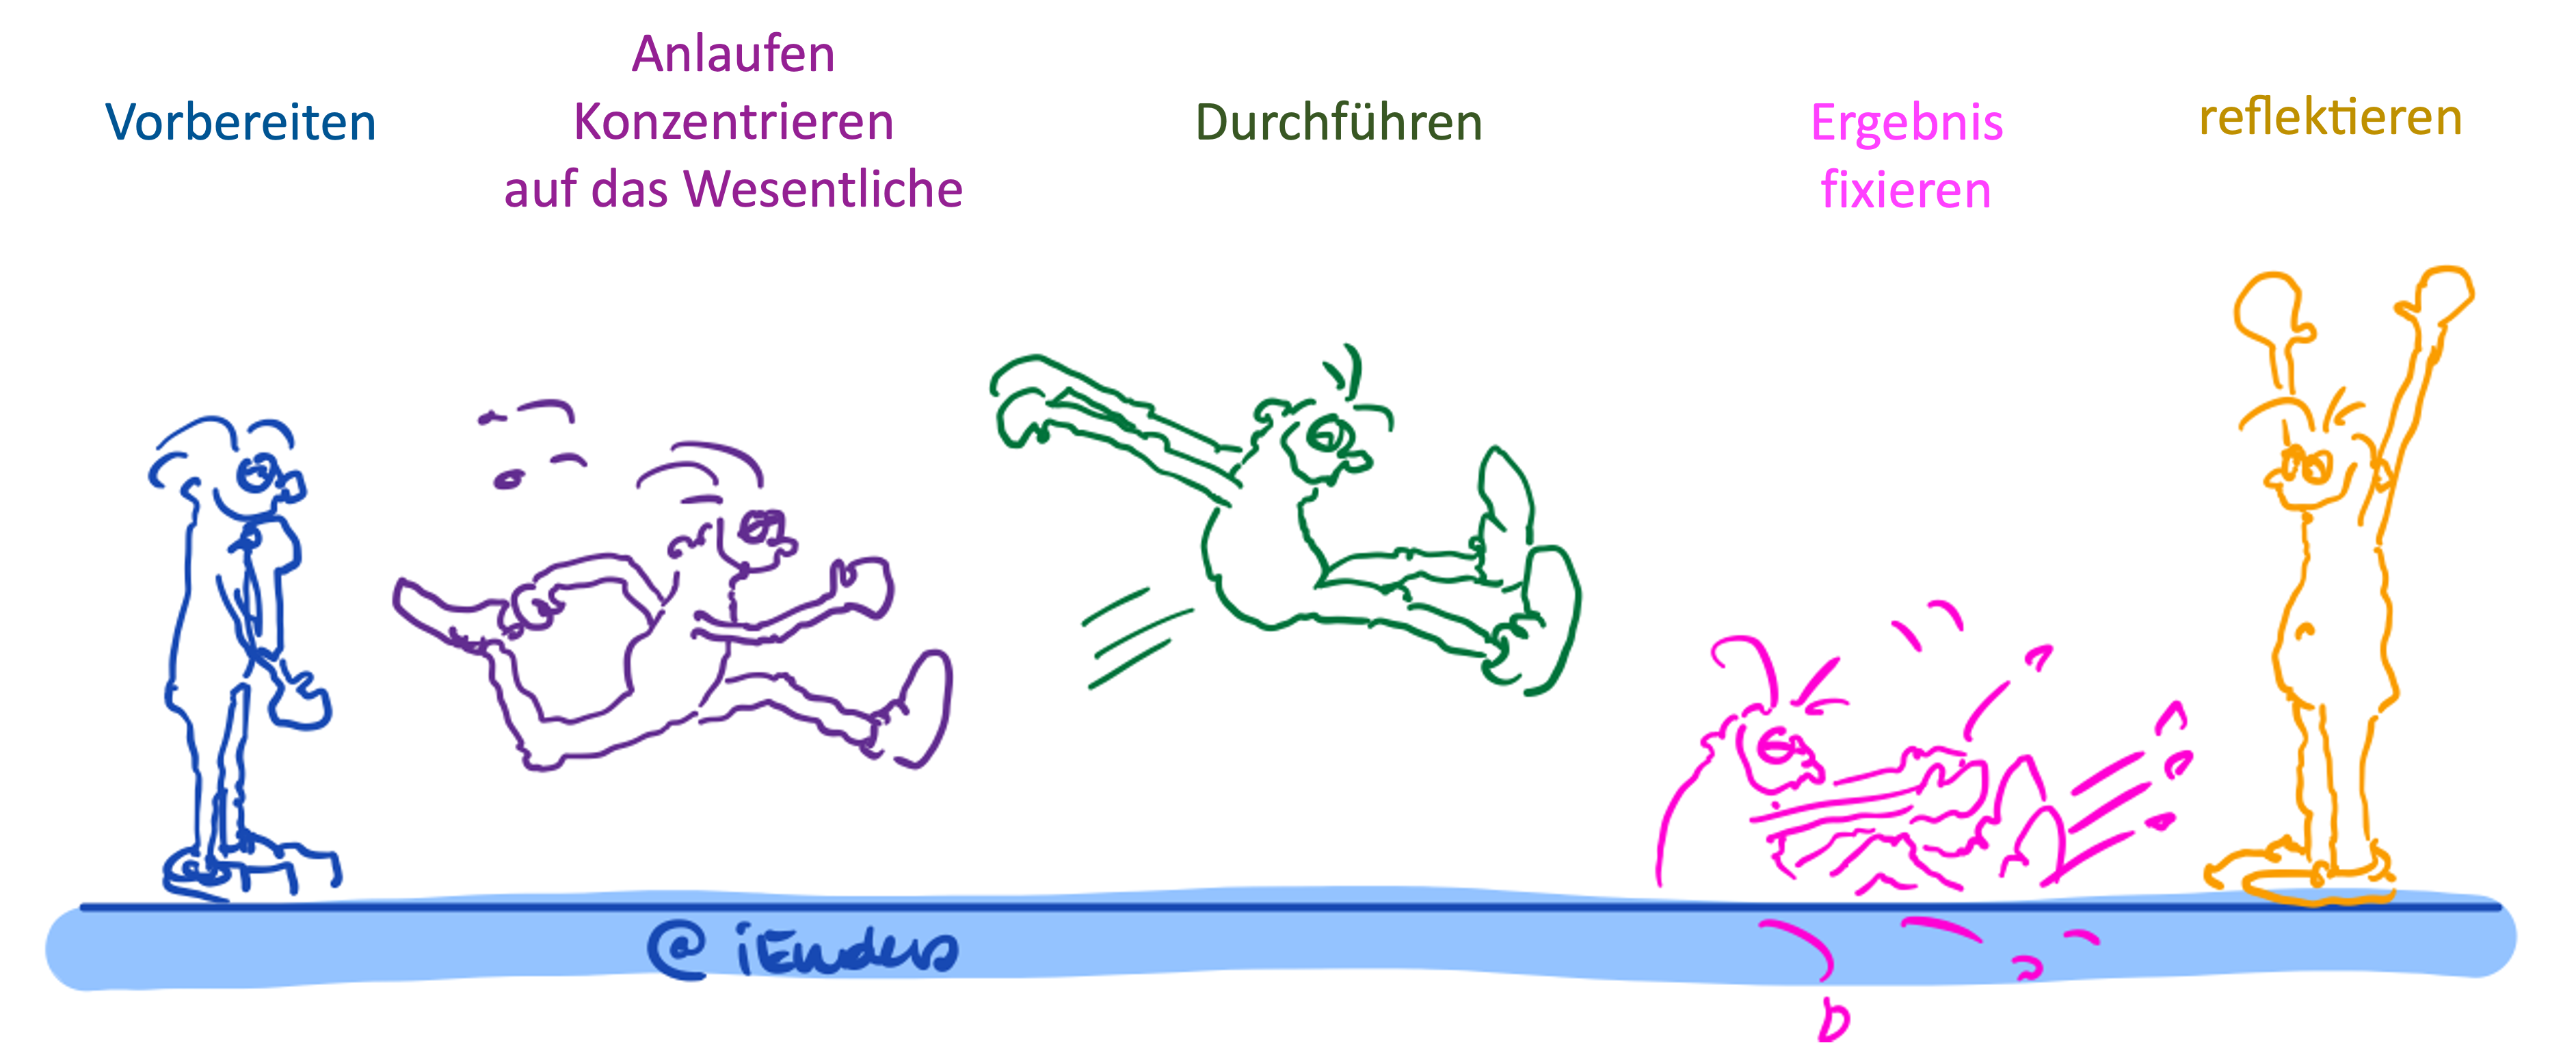
\includegraphics[scale=.5]{Artikulationsschema.png}
	\caption{Grundstruktur eines Artikulationsschemas}
	\label{fig:Artikulationsschema}
\end{figure}


\mip
Insgesamt sind die Schemata als idealtypisch anzusehen und
nicht schablonenhaft zu verwenden.
In der Realit\"{a}t treten vielf\"{a}ltige Modifikationen auf:
\begin{itemize}
	\item
	Unterschiedliche Gewichtung der Stufen.
	\item
	Flie{\ss}ender \"{U}bergang oder Verschmelzung von Stufen.
	\item
	Weglassen oder Mehrmaliges Durchlaufen von Stufen.
\end{itemize}

%Vergleichende \"{U}bersicht:
% Siehe \cite[S.\ 200]{BleichrothDahnckeJung}
% \cite[S.\ 215]{Willer}.

Die Struktur von Artikulationsschemata ist grundlegend immer \"{a}hnlich und anschaulich in Abbildung \ref{fig:Artikulationsschema} dargestellt.

\mip
Die in den folgenden Beispielen vorgestellten Schemata \"{a}hneln
einander alle. Es ist eine allgemeine Dramaturgie
wie beim Weitsprung (Vorbereiten -- Anlaufen -- Konzentrieren
auf das Wesentliche -- Durchf\"{u}hren -- Ergebnis fixieren --
reflektieren) oder bei einer
Schulaufsatz-Erlebniserz\"{a}hlung (Einleitung -- Hauptteil -- Schluss) zu erkennen.

\subsection{Herbart: Die Formalstufen}
Die Idee, Unterricht oder -- allgemeiner -- das Lernen, auf diese
Weise planerisch zu gestalten, geht auf Johann Friedrich
Herbart (1776 -- 1841, 1806: Allgemeine P\"{a}dagogik) zur\"{u}ck.
So wird die p\"{a}dagogische Schule, die diese Gedanken (zum Teil
\"{u}berzeichnet-formalisiert) vertritt,
auch die {\em Schule der Herbartianer} genannt.
Ihre wichtigsten Vertreter sind Rhein und Ziller.

\begin{quote}
	\bf Idee: Das Atmen des Geistes
\end{quote}

\begin{enumerate}
	\item
	{\bf Vertiefung (Einatmen)}
	\begin{enumerate}
		\item[1.]
		{\bf Klarheit} Der einzelne Gegenstand wird klar und in allen
		Einzelheiten vor Augen gef\"{u}hrt.
		\item[2.]
		{\bf Assoziation} In freier Gedankenbildung werden alle nur
		denkbaren geistigen Erkenntnisse aus der Erinnerung in
		Verbindung zu den bereits vorhandenen Elementen gesetzt.
	\end{enumerate}

	\item {\bf Besinnung (Ausatmen)}
	\begin{enumerate}
		\item [3.]
		{\bf System} Die Verbindung des erkannten einzelnen zu den
		bisherigen Erkenntnissen wird systematisch aufbereitet, eine
		Einordnung findet statt.
		\item[4.]
		{\bf Methode} Die Erkenntnis wird angewandt, wobei sie sich
		verifiziert.
	\end{enumerate}
\end{enumerate}

\subsection{Heinrich Roth (1963): Die Lernstufen}
Die diesem Lernstufenschema zugrundeliegende Idee besteht
darin, den Lernvorgang des Sch\"{u}lers psychologisch geeignet zu
begleiten. Es gr\"{u}ndet sich letztlich auf umfassende empirische
Studien zu Lernvorg\"{a}ngen.

\mip
Es ist typisch f\"{u}r eine Unterrichtsstunde,
in der eine Erkenntnis oder Einsicht gewonnen werden soll, es
eignet sich insbesondere also f\"{u}r den naturwissenschaftlichen
Unterricht und die Physik.
Andererseits ist das Schema sehr allgemein gehalten, so dass es
vielf\"{a}ltig anwendbar ist.

\begin{enumerate}
	\item {\bf Stufe der Motivation} Zum Begriff der Motivation
	vergleiche weiter unten.
	
	\item {\bf Stufe der Schwierigkeiten}
	\begin{itemize}
		\item Unter Umst\"{a}nden verschr\"{a}nkt mit der Stufe der Motivation.
		\item Es handelt sich um eine Art Innehalten in Form eines
		Zwischenstopps nach der Stufe der Motivation.
		Das Ziel tritt klar vor Augen.
		\item Der Sch\"{u}ler soll sich am Ende des Einstiegs der
		Schwierigkeiten, des Problems, bewusst sein.
		Das zu l\"{o}sende Problem muss isoliert und klar formuliert werden.
		Erste L\"{o}sungsversuche sollten zur\"{u}ckgestellt werden.
		\item Das Problem erscheint
		(evtl. als Thema der Unterrichtsstunde)
		an der Tafel oder auf der Folie.
		\autocite[S. 207]{BleichrothDahnckeJung}
	\end{itemize}
	
	\item {\bf Stufe der L\"{o}sung}
	
	Sie bildet den eigentlichen inhaltlichen Mittelpunkt der Stunde.
	Im Physikunterricht wird hier im Allgemeinen experimentiert.
	
	Je nach Unterricht kann die konkrete Ausgestaltung
	unterschiedlich angelegt sein:
	
	\begin{itemize}
		\item Induktive Erarbeitung eines Gesetzes im Experiment
		(Hooke'sches Gesetz, ohmsches Gesetz, Gesetz \"{u}ber die Siedetemperaturerniedrigung bei Druckerh\"{o}hung)
		$\to$ Elementarisierung.
		\item Einsicht in einen technischen Funktionszusammenhang
		(Otto-Motor, Elektromotor, hydraulische Hebeb\"{u}hne, Glasfaserkabel).
		\item Einf\"{u}hrung von Begriffen (Verdunstung, W\"{a}rmeleitung) oder
		Gr\"{o}{\ss}en (Kraft, Spannung), Einheiten und Messverfahren.
		\item Messung einer Konstanten.
	\end{itemize}
	
	\item {\bf Stufe des Tuns und Ausf\"{u}hrens}
	\begin{itemize}
		\item Die Halbleiterdiode, der Elektromotor wird tats\"{a}chlich eingesetzt.
		\item Best\"{a}tigungsversuch.
	\end{itemize}
	
	\item {\bf Stufe des Behaltens und Ein\"{u}bens}
	
	Psychologische Erkenntnis:
	Durch Wiederholung kann das Behalten im
	Ged\"{a}chtnis wesentlich gef\"{o}rdert werden.
	
	\begin{itemize}
		\item (M\"{u}ndliche) Wiederholung (in eigenen Worten)
		\item \"{U}bung, \"{U}bungsaufgaben
		($\to$ Typisch im Mathematikunterricht).
		\item Anwendung in Natur, Alltag und Technik (Verdunstung $\to$
		Schwei{\ss}bildung, Hydraulische Presse $\to$ Autohebeb\"{u}hne,
		3.\ Bewegungsgleichung $\to$ Fahrschulformel)
		\item Variation
		\item Beispiele zu dem Gesetz,
		Spezialf\"{a}lle (Auftrieb $\to$ Schweben).
		\item Eintrag ins (Merk-)Heft.
		\item Hausaufgabe.
		\item Schulbuch-Abgleich.
	\end{itemize}
	
	\begin{beisp}
		Knoff-Hoff-Show:
	Nach jeweils einem Thema werden die Inhalte in
	Kurzsequenzen wiederholt.
	\end{beisp}
	
	\item {\bf Stufe der Integration, der \"{U}bertragung und
	der Bereitstellung}
	
	\begin{itemize}
		\item Eventuell Nahtstelle mit Anfangsphase der Folgestunde
		\item Integration (Wagenschein: Herstellung des Systems):
		Der neu gelernte Inhalt wird in das System der fr\"{u}her
		gelernten Inhalte auf vielf\"{a}ltige Weise
		eingef\"{u}gt (Verkn\"{u}pfung, Assoziation, Ordnung,\dots).
		\item \"{U}bertragung des Inhalts auf neue Sachverhalt
		(Beachte: Nach W.\ Jung ist Transfer i.~A.\ nur sehr
		beschr\"{a}nkt m\"{o}glich).
		\item Element der Lernzielkontrolle.
	\end{itemize}
\end{enumerate}

\subsection{Normalverfahren: Orientierung am naturwissenschaftlichen Erkenntnisweg}
Naturwissenschaftlicher Unterricht soll neben den fachlichen Inhalten (materiale Bildung) auch Kenntnisse und Kompetenzen im Hinblick auf die Arbeitsweisen der Fächer vermitteln (formale Bildung). Einige Artikulationsschemata aus den Didaktiken der Naturwissenschaften orientieren sich daher am naturwissenschaftlichen Erkenntnisweg. Die zugrundeliegende Idee besteht darin, das Grundmuster naturwissenschaftlicher Erkenntnis in Unterrichtsabl\"{a}ufe einzupassen. 

\mip
Die ersten derartigen Schemata formulierten Dewey (1910) und Kerschensteiner (1914). Diese rezipierte Hans Mothes 1968 im von ihm so bezeichneten \textbf{Normalverfahren}. Es enthält folgende Stufen in Anlehnung an die induktive Vorgehensweise der fachwissenschaftlichen Erkenntnisgewinnung:

\begin{enumerate}
	\item {\bf Problemfrage}
	\item {\bf Meinungsbildung}
	\item {\bf Die Nachpr\"{u}fung des auf der Stufe der Meinungsbildung gewonnenen Urteils}, welches die Schritte \emph{deduktive \"{U}berlegungen}, \emph{Versuchsplanung},  \emph{eigentliches Experiment} und \emph{Urteil Erkenntnissatz} beinhaltet
	\item {\bf R\"{u}ckkehr vom Gedankenger\"{u}st der Erkenntnis zur Wirklichkeit}
	\item {\bf Ma\ss nahmen zur Festigung des Unterrichtsergebnisses}
\end{enumerate}

Weiterentwicklungen des Normalverfahrens finden sich bei \textcite{DuitHausslerKircher}, \textcite{Ploeger} sowie bei Bauer (1984). Sie betonen die aktive Beteiligung der Schüler auf den Erkenntnisweg. Der schematische Ablauf der Unterrichtseinheit weicht jedoch nicht wesentlich vom Normalverfahren ab.

\mip
{\bf Kritikpunkte am Normalverfahren:}
\begin{itemize}
	\item Es ist fraglich, ob jedoch dieses Verfahren tats\"{a}chlich ein Abbild der Wissenschaft ist, da f\"{u}r Forschung eine Idee notwendig ist, was man \"{u}berhaupt untersuchen will. Im Gegensatz dazu inszeniert der Lehrer den Unterricht h\"{a}ufig so, als w\"{a}ren ihm die zu ermittelnden Sachverhalte noch nicht bekannt.
	\item Es gibt weitere naturwissenschaftliche Erkenntniswege als den Vierschritt \textbf{\say{Problem -- Hypothese -- Experiment -- Verifikation}}. Daraus folgt auch, dass es kein Abbild einer einheitlichen naturwissenschaftlichen Methode im Unterricht geben kann.
	\item Das routinehafte Vorgehen im Sinne eines \say{normal}, also immer anzuwendenden Verfahrens fördert keineswegs die formale Bildung der Schüler, selbst wenn diese die konstituierenden Schritte selbstständig ausführen. Dies belegen auch die stetig abnehmenden Ergebnisse internationaler Schulleistungsstudien.
	\item Vielmehr ist \emph{eigenständiges} naturwissenschaftliches Vorgehen, losgelöst von Standardschemata, im Unterricht zu fördern. Im Sinne der \emph{kognitiven Meisterlehre} bzw. des \emph{Scaffoldings} werden die Schüler dabei, wo erforderlich, von der Lehrkraft unterstützt. Die naturwissenschaftlichen Arbeitsweisen erfahren sie während des aktiven Tuns.
\end{itemize}



\subsection{Fallstudie: Die Phase der Motivation}
,,Motivare'' hei{\ss}t ,,in Bewegung versetzen''.
In der Psychologie ist der Motivationsbegriff nicht einheitlich
definiert.
\bip
Berlyne (1974) sieht den kognitiven Konflikt als Kern der
(sachbezogenen) Motivation an.
Kognitive Konflikte entstehen, wenn sich Wahrnehmungen
nicht in den vorhandenen Wissens- oder Erfahrungszusammenhang
einbetten lassen, sie folgen dabei einigen Grundmustern:

\begin{itemize}
	\item {\bf \"{U}berraschung:}
	Konflikt zwischen Erwartung und Erfahrung.
	
	Man erwartet aufgrund gefestigter Erfahrung ein anderes
	Ergebnis als es tats\"{a}chlich erfolgt.
	
	Das Auftreten h\"{a}ngt von der vorhandenen Erfahrung
	(Lebensalter, Jahrgangsstufe) ab.
	\begin{beisp2}
		\begin{itemize}
		\item
		Ein Schiff aus Eisen geht nicht
		unter (Schwerkraft $\ctr$ Auftrieb).
		\item
		Ein Glas Wasser flie{\ss}t nicht aus, wenn es mit einer St\"{u}ck
		Karton abgedeckt und vorsichtig umgedreht wird
		(Schwerkraft $\ctr$ Adh\"{a}sionskr\"{a}fte).
		\item
		Ein Phasenpr\"{u}fer leuchtet auf, wenn man mit der anderen Hand
		die Wasserleitung ber\"{u}hrt. (Wasserleitung $\ctr$ Erdung)
		\item
		Huckepackball: Ein kleiner Superball wird auf eine gro{\ss}en gelegt,
		beide werden in dieser Lage fallen gelassen.
		Der kleine Ball erreicht nach dem Aufprall ein
		Vielfaches der Ausgangsh\"{o}he
		(Energiesatz $\ctr$ Energie\"{u}bertragung).
		\item
		Wasser in einem d\"{u}nnen R\"{o}hrchen steht h\"{o}her als in der Umgebung.
		(Hydrostatisches Grundgesetz $\ctr$ Kapillarit\"{a}t)
		\item
		Ein Aluminiumring wird vom Pol eines Elektromagneten beim
		Einschalten abgesto{\ss}en
		(Aluminium ist nicht ferromagnetisch $\ctr$ Lorentzkr\"{a}fte).
		\end{itemize}
	\end{beisp2}
	
	
	\item {\bf Zweifel:} Konflikt zwischen Glauben und Nichtglauben
	
	Zweifel ensteht bez\"{u}glich einer nicht direkt nachpr\"{u}fbaren
	Aussage, weil sie Resultat einer Idealisierung oder theoretischen
	\"{U}berlegung ist.
	
	\begin{beisp2}
		\begin{itemize}
		\item
		Ein reibungsfrei beweglicher Wagen f\"{a}hrt gleichf\"{o}rmig weiter,
		wenn er sich selbst \"{u}berlassen wird.
		\item
		Alle K\"{o}rper (auch Menschen) ziehen einander an.
		\item
		Ein G\"{u}terwagen kann mit der Hand gezogen werden.
		\item
		Wir bewegen uns mit \SI{100}{\kilo\meter\per\hour} um die Erdachse und mit \SI{30}{\meter\per\second}
		um die Sonne.
		\end{itemize}
	\end{beisp2}
	
	
	
	\item {\bf Ungewissheit, Verwirrung:}
	Konflikt zwischen mehrdeutigen oder unvollst\"{a}ndigen Erfahrungen.
	
	\begin{beisp2}
		\begin{itemize}
		\item
		Materie kann als Kontinuum oder als k\"{o}rnige Struktur aufgefasst
		werden.
		\item
		Zieht man am offenen Ende eines Zwirns an einer N\"{a}hfadenrolle,
		so stellt sich die Frage, ob sich die Rolle sich her- oder wegbewegt.
		\item
		Auf einen wasserbedeckten Teller wird eine Kerze gestellt und dann
		ein Glasgef\"{a}{\ss} \"{u}bergest\"{u}lpt.
		Warum steigt das Wasser auf? (Chemische Effekte $\ctr$
		W\"{a}rmeausdehnungseffekte)
		\item
		Historisch: Licht hat Wellen- oder Teilchencharakter.
		\end{itemize}
	\end{beisp2}
	

	
	\item {\bf Irrelevanz:}
	Bisherige Informationen sind irrelevant
	\begin{beisp}
		Rutherford Streuversuche.
	\end{beisp}
	
	\item {\bf Verunsicherung, Ratlosigkeit:}
	\begin{beisp2}
			\begin{itemize}
		\item
		Kann man zu einem Regenbogen spazieren?
		\item
		Ist ein Lichtstrahl sichtbar?
		\item
		Schwimmt Aluminium im Wasser?
	\end{itemize}
	\end{beisp2}

	
	\item {\bf Staunen, Wundern}
	\begin{beisp2}
		\begin{itemize}
			\item Was passiert, wenn die Erde aufhört, sich zu drehen?
			\item Warum ist der Himmel nicht violett?
			\item Perspektivwechsel: Wie sieht eine Ameise die Welt?
		\end{itemize}
	\end{beisp2}
	\item {\bf Paradoxie, Zwiespalt}
	\begin{beisp2}
		\begin{itemize}
		\item
		Das Hydrostatische Paradoxon: Bei gleicher Wasserh\"{o}he ist der
		Druck am Boden eines Gef\"{a}{\ss}es unabh\"{a}ngig von Volumen oder Form
		des Gef\"{a}{\ss}es.
		\item
		Das Aerodynamische Paradoxon: Man bl\"{a}st durch den Spalt zwischen
		zwei einander zugewandt gew\"{o}lbten Kartons.
		Die Kartons bewegen sich aufeinander zu.
		(Statischer Druck $\ctr$ Staudruck).
		
		\item
		Das Zwillingsparadoxon der Allgemeinen Relativit\"{a}tstheorie.
		
		\item
		Historisch: Olbers'sches Paradoxon (1826).
		\end{itemize}
	\end{beisp2}
	
	
	
	\item {\bf Neuigkeitsgehalt, Aktualit\"{a}t}
	\begin{beisp2}
		\begin{itemize}
			\item Erdbeben, Tsunami
			\item Klimawandel, Energietechnologien
			\item Mond- und Marsmissionen
			\item Quantencomputer
		\end{itemize}
	\end{beisp2}
\end{itemize}

\subsection{Fallstudie: Einstiege in eine Unterrichtseinheit}

Dieser Begriff ist weniger anspruchsvoll als der der Motivation.
Mit dem Einstieg nimmt der Unterrichtsgang den Anfang eines
roten Fadens (des Lernprozesses) auf.

Spielarten von Einstiegen:
\begin{itemize}
	\item
	{\bf Einstieg \"{u}ber eine Beobachtung in der Natur}
	\begin{beisp2}
		\begin{itemize}
		\item
		Lichtstrahlen im Wald.
		\item
		Regenbogen.
		\end{itemize}

	\end{beisp2}
	
	
	\item {\bf	Einstieg \"{u}ber eine Beobachtung im Haushalt}
	\begin{beisp2}
		Dampfkochtopf, K\"{u}hlschrank, Fernseher, Heizung.
	\end{beisp2}
	
	\item {\bf Einstieg \"{u}ber eine Beobachtung in der Freizeit}
	\begin{beisp2}
		Fahrrad, Schwimmen.
	\end{beisp2}
	
	\item {\bf 	Einstieg \"{u}ber Handwerk und Technik}
	\begin{beisp2}
			\begin{itemize}
	\item
	Metallbau: Schwei{\ss}en, Korrosion.
	\item
	Elektro: Installation
	\item
	Bau: Kran, Hydraulische Maschinen, W\"{a}rmeisolation, \dots
	\end{itemize}
	
	\end{beisp2}

	\item {\bf
	Einstieg \"{u}ber eine (qualitative oder quantitative)
	Versuchsreihe.}
	\begin{beisp2}
		\begin{itemize}
			\item
			Welche Stoffe leiten den el.\ Strom?
			\item
			Hooke'sches Gesetz.
			\item
			Ohm'sches Gesetz.
	\end{itemize}
	\end{beisp2}

	
	\item {\bf 	Einstieg \"{u}ber einen Schl\"{u}sselbegriff oder -gegenstand}
	
	\item {\bf 	Einstieg \"{u}ber ein aktuelles Ereignis}
	\begin{beisp2}
			\begin{itemize}
	\item
	Baugenehmigung f\"{u}r Physik-Projekt (Garching),
	\item
	Bau eines Kraftwerks, \"{U}berlandleitung,
	\item
	Weltraumfahrt (Marslandung)
	\item
	Astronomie (Finsternisse, Kometen,\dots)
	\end{itemize}
	\end{beisp2}

	
	\item {\bf 	Einstieg \"{u}ber Vergegenw\"{a}rtigung einer historischen Begebenheit}
	\begin{beisp2}
		z. B.\ wegen Jahrestag einer Entdeckung, Briefmarkenherausgabe,
	Biographie eines Naturforschers)
				\begin{itemize}
	\item
	Oersted-Versuch: Induktion in ruhenden Leitern.
	\item
	Newton'sches Gravitationsgesetz.
	\item
	Entdeckung der Radioaktivit\"{a}t: Bequerel.
	\item
	Erfindung des ersten Transistors: 23.12.1947.
	\item
	Auffindung der R\"{o}ntgenstrahlung: 7.11.1895.
	\end{itemize}
	\end{beisp2}
	

	{\bf
	\item
	Einstieg \"{u}ber ein Ereignis im Jahreslauf
	(Bleigie{\ss}en an Silvester, Feuerwerk, Asphaltspiegelungen im Sommer)
	
	\item
	Einstieg \"{u}ber ein pers\"{o}nliches Erlebnis.
	
	\item
	Einstieg \"{u}ber einen Zeitungs- oder Zeitschriftenartikel, Radio- oder Fernsehbericht, Buchlekt\"{u}re.}

\end{itemize}

\subsection{Fallstudie: Das Aufstellen einer Vermutung bzw. Hypothese}
Im Sinne Kerschensteiners  steht vor der schnellen Beantwortung einer
Frage an die Natur durch das Experiment die Aufstellung m\"{o}glicher Ergebnisse
\bip
\begin{beisp2}
	\begin{itemize}
\item \textbf{Fadenpendel:}
Welche Gr\"{o}{\ss}en sind entscheidend?
\item \textbf{Parallelschaltung:} Welcher Gesamtwiderstand ergibt sich,
wenn zwei Widerst\"{a}nde parallel geschalten werden? Vermutungen:
    \begin{itemize}
      \item Mittelwert $\frac{R_1 + R_2}2$,
      \item $\frac{R_1+R_2}4$,
      \item $R_1 \cdot R_2$,
      \item $\frac{1}{R} = \frac{1}{R_1} + \frac{1}{R_2}$.
    \end{itemize}
\item \textbf{Widerstand eines Drahtes:} Von welchen Gr\"{o}{\ss}en h\"{a}ngt er ab?
\item \textbf{Mondphasen:}
\begin{itemize}
  \item Erdschatten,
  \item Halbseitiges Leuchten,
  \item Halbseitige Beleuchtung durch die Sonne.
\end{itemize}
\item \textbf{\"{A}therhypothese}
\item \textbf{Kontinuumshypothese}
\item \textbf{Museum f\"{u}r Mensch und Natur in M\"{u}nchen:} Der Besucher (Kind) muss erst
seine Vermutungen \"{u}ber bestimmte Fragen:
\begin{itemize}
\item Welche der gezeigten Tiere sind Fr\"{o}sche?
\item Welche der gezeigten Tiere haben Knochen?
\item Welche Tiere sind am schnellsten?
\end{itemize}
\"{a}u{\ss}ern, bevor die Frage aufgel\"{o}st wird.
\end{itemize}
\end{beisp2}



%------------------------------------------------------------------------------------------------------------------------------------------------------------------------
\bip\bip
\section{Unterrichtsverfahren}\label{Verfahren}

Synonym werden auch die Begriffe
,,Methodenkonzept'', ,,Methodisches Konzept'' oder ,,Unterrichtsgang'' verwendet.
Unterrichtsverfahren beschreiben nicht so sehr den zeitlichen Ablauf,
sondern eher den grundlegenden Ductus (Gang) eines Unterrichts.
Empirische Untersuchungen zum Erfolg der Unterrichtsverfahren
sind schwierig, sie erfolgen an simplifizierten Verfahren.

Es besteht ein grundlegendes Spannungsfeld:
\mip
\begin{center}
\begin{tabular}{ |p{.5\textwidth}| p{.5\textwidth}| }
\hline
 Entdeckender Unterricht
&
Darbietender Unterricht
\\ \hline \hline
 Probleml\"{o}sendes Unterrichtsverfahren
&
Darstellend-entwickelndes Unterrichtsverfahren
\\ \hline
 Die Sch\"{u}ler bet\"{a}tigen sich selbst als ,,Physik-Erkennende''.
&
Die Sch\"{u}ler lernen (rezipieren) den Lernstoff.
\\ \hline
 Prozessziele (Methodische Denken) &
Konzeptziele (Wissen, Kenntnisse)
\\ \hline
 Idealform, aufw\"{a}ndig
&
Realit\"{a}tsbedingt, \"{o}konomisch
\\ \hline
 Weniger Lenkung, intrinsische Motivation
&
Mehr Lenkung
\\ \hline
 Eher Sch\"{u}lerversuche
&
Eher Lehrerversuche
\\ \hline
 Exponent: J.\ Bruner (am): Gedanken zu einer Theorie des Unterrichts
,,Entdeckenden Lernens''. &
Exponent: D.J.\ Ausubel (kan): Psychologie des Unterrichts
\\ \hline
 Medieneinsatz: Experimente, Materialien aus dem Alltag
&
Medieneinsatz: Vorausorganisatoren, Arbeitsbl\"{a}tter
\\ \hline

{Besondere Auspr\"{a}gungen: \newline
Genetischer Unterricht \newline
Forschender Unterricht \newline
Nacherfindender Unterricht \newline
Historisierender Unterricht \newline
Modellmethode
}
&
{Besondere Auspr\"{a}gungen: \newline
Sinnvoll-\"{u}bernehmender Unterricht \newline
Fragend-entwickelnder Unterricht \newline
Nachmachender Unterricht \newline
Induktiv-deduktives Verfahren \newline
Synthetisch-analytisches Verfahren
}
\\ \hline
\end{tabular}\end{center}

Langfristig wird ein Physikunterricht von einer
Verschr\"{a}nkung und Variation dieser beiden grundlegenden
Formen gepr\"{a}gt sein.

Dieser Abschnitt stellt einige Beispiele vor.

\subsection{Das genetische Unterrichtsverfahren}

Begr\"{u}nder und spiritus rector: Martin Wagenschein.
\bip
\begin{tabular}{r p{12cm}}
1896 &  Geburt. Studium der Physik und Mathematik,
Promotion in Physik.
\\
$\approx$1920 &  Unterricht an staatlichen Gymnasien,
Erfahrungen in der ,,Freien Schulgemeinde Odenwaldschule''
Paul Geheebs.
\\
1945 &  Schulversuche, Bildungspl\"{a}ne.
\\
1951 &  T\"{u}binger Resolution.
\\
1960--65 &  Ausschuss ,,H\"{o}herer Schule'' des Deutschen Ausschusses.
\\
1956 -- &  Honorarprofessor T\"{u}bingen, 20 Jahre Seminar.
\\
1978 &  Ehrendoktor TH Darmstadt.
\\
Ostern 1988 &  gestorben.
\end{tabular}

\bip
Drei Aspekte des genetischen Unterrichts (Genese = Entstehung):
\begin{itemize}
\item Individual-genetischer Aspekt: Die Genese der Erkenntnis im
Sch\"{u}ler.
\item Logisch-genetischer Aspekt: Die allgemeine Genese der
Erkenntnis.
\item Historisch-genetischer Aspekt: Genese der Erkenntnis in der
Entwicklung der Wissenschaft.
\end{itemize}

\bip
Thesenartige Umschreibung der ,,Botschaft'' Wagenscheins:
\begin{itemize}

\item Physikalisches Handeln entfaltet p\"{a}dagogische  Wirkung
schlechthin. Physik ist nicht einfach ein Transportgut der P\"{a}dagogik.

\item Physik braucht Freiraum (von Schulsystem, Lehrpl\"{a}nen,
Zeitzw\"{a}ngen, Vollst\"{a}ndigkeitsbestreben.
\item Der Physikunterricht muss sich auf die Trias
\begin{quote}
exemplarisch --- sokratisch --- genetisch
\end{quote}
gr\"{u}nden.


\item Exemplarisch: Der Prozess des Werdens von Physik im Menschen
wird anhand von Beispielen erlebt.
Ein einzelnes Ergebnis (Erkenntnismethode,
Arbeitsform) ist repr\"{a}sentativ f\"{u}r das System der Gesamtphysik.
\item Sokratisch  (Sokrates-Dialoge, von Platon \"{u}berliefert):
Der Lernende findet die L\"{o}sung selbst, begleitet durch geschickte
Fragen und Impulse, keine Mitteilung von Informationen.


\item Genetisch: Physik ist ein Prozess, nicht eine Wissenssammlung:
\begin{quote}
Verstehen (lernen) statt Wissen (lernen)  (Genetisch statt
Enzyklop\"{a}disch)
\end{quote}
(Pestalozzi: Die Schule bringt dem Menschen das Urteil in den Kopf,
ehe er die Sache sieht und kennt.)
\mip
Genetischer Unterricht ber\"{u}cksichtigt das, was die
Sch\"{u}ler schon wissen, er verfr\"{u}ht keine Ergebnisse, sondern zielt
auf deren Einwurzelung, ohne die es keine Formatio gibt.
 \autocite[S.\ 107 oben]{DuitHausslerKircher}.

\item ,,Rettet die Ph\"{a}nomene'' Die Sch\"{u}ler m\"{u}ssen die Welt
erleben, bevor sie sie (analytisch) erkl\"{a}rend durchdringen
\autocite[S.\ 90,104]{WagenscheinNSV}.

\item Die Selbstzweck-Mathematisierung muss zur\"{u}ckgefahren werden.

\item Die drei Phasen des exemplarisch-sokratisch-genetischen Unterrichts:
\begin{enumerate}
\item Einstieg: \say{Wir steigen vom Seltsamen ins Elementare (von
der Todesschleife zum Tr\"{a}gheitssatz) hinab.}
\autocite[S.\ 205]{WagenscheinPDP}
\item Bildung und \"{U}berpr\"{u}fung von Hypothesen,
\item Vertiefung, Systematisierung (wenig betont in Wagenscheins
Beispielen)
\end{enumerate}

\item Organisatorisch: Mindestens Doppelstunden, besser
Epochalunterricht, Sch\"{u}ler gruppieren sich seminarartig um die
Tische.
\end{itemize}

\bip\bip
\subsection{Forschender Unterricht}
Begründer: Georg Kerschensteiner

\begin{tabular}{r p{.7\textwidth}}
29.7.1854 &
Geboren in M\"{u}nchen, Ausbildung zum Volksschullehrer,
sp\"{a}ter Gymnasiallehrer.
\\
1874 -- 1880 &  Lehrer an Volksschulen und Gymnasien
in/bei M\"{u}nchen, Augsburg, N\"{u}rnberg, Schweinfurt, M\"{u}n\-chen.
\\
1884 &  Doktorarbeit in Mathematik
\\
1885 -- 1919 &  Leiter des Volks- und Berufsschulamtes,
Stadtschulrat, \"{U}berdenken der Organisation des Schulwesens.
\\
1910 &  Mitinitiator einer Lehrplanreform, die die Bedeutung des
naturwissenschaftlichen Unterrichts
hervorhebt.
(Ausl\"{o}sung des ,,M\"{u}nchner Schulstreits'').
\\
1914 &  \say{Wesen und Wert des naturwissenschaftlichen
Unterrichts}.
\\
1919 -- 1928 &  Universit\"{a}tsprofessor, theoretische Arbeit,
Reisen in die USA, tr\"{a}gt zur Reform des Schulwesens bei.
\\
1926 &  Hauptwerk ,,Theorie der Bildung''.
\\
15.1.1932 &  Gestorben in M\"{u}nchen.
\end{tabular}

\bip
Kerschensteiners Ideen bedeuten insgesamt eine Antwort auf das
im 19.\ Jahrhundert vorherrschende Humboldt'sche Bildungsideal
mit seiner geistig-intellektuellen humanistischen
Ausrichtung, das auch die Schullandschaft pr\"{a}gte.

\bip
Idee des Forschenden Lernens (Discovery learning) nach Kerschensteiner, Dewey, Kilpatrick.
\begin{itemize}
\item Betonung auch der Handarbeit: K\"{o}rperliche Fertigkeiten sind
ein Bestandteil der Menschenbildung.
$\to$ Werkunterricht, Zeichenuntericht, Arbeitsschulbewegung.
\item Begr\"{u}ndung des naturwissenschaftlichen Unterrichts und
seines Bildungswerts.
Naturwissenschaften sind integraler Bestandteil der Menschenbildung.
\item Betonung der naturwissenschaftlichen Methode der
Erkenntnisgewinnung im Unterricht.
\item Betonung der Berufsbildung: Zur Berufsausbildung geh\"{o}rt
eine umgebende allgemeinere Geistesbildung.
Kerschensteiner ist der ,,Vater der Berufsschule''.
\item Soziale Bildung: Ausbildungsziel in der (Berufs-)Schule ist
der ,,Staatsb\"{u}rger in Verantwortung'' $\to$ Sozialkundeunterricht.
\item Selbstt\"{a}tigkeit  $\to $ Sch\"{u}lerexperimente.
\item Anschauung, au{\ss}erschulische Lernorte!
\item Reform des Schulwesens, Umgestaltung der Forbildungsschulen
in Berufsschulen.
\item Abfolge von: Problem -- Hypothese -- Verifikation/Falsifikation.
(Vgl.\ auch das Stufenschema von H.F.\ Bauer bzw.\ Pl\"{o}ger).
\item Kritik: Vernachl\"{a}ssigung der geschichtlichen und
musischen Bildung.
\end{itemize}


\bip\bip
\subsection{Nacherfindender Unterricht}
\begin{itemize}
\item Die Fragestellung besteht in der Konstruktion eines
technischen Ger\"{a}tes
\begin{beisp2}
	El.\ Klingel, Elektromagnet, Flaschenzug,
Messger\"{a}t, Thermometer, Morse-Apparat, optische Ger\"{a}te,
hydraulische Presse, Kaffeemaschine.
\end{beisp2}

\item Artikulation:
\begin{enumerate}
\item Es werden Pl\"{a}ne entworfen.
\item \"{U}berdenken der Realisierungsm\"{o}glichkeiten.
\item Tats\"{a}chliche Konstruktion
\item Funktionstest
\item Verbesserung des Ger\"{a}tes: Wie kann es einfacher, stabiler,
billiger, bedienungsfreundlicher, zuverl\"{a}ssiger, energiesparender,
umweltfreundlicher gestaltet werden?
\item Das Prinzip der Handlungsorientierung wird verwirklicht.
\item Lernziele bestehen in dem Bewusstsein, dass technische Ger\"{a}te
leichter durchschaubar sind, als man vermutet (vgl.\ auch
Black-Box-Prinzip).
\item Problem: Sch\"{u}lerbaupl\"{a}ne sind komplex angelegt, sie sind
vergleichsweise schwer umsetzbar.
\end{enumerate}
\end{itemize}

%\section{Fragemethode}
%\begin{itemize}
%\item Es handelt sich um eine stark formalisierte
%,,Was-bin-ich-Strategie''.
%(Erinnerung: Sokratischer Unterricht)
%\item Der Lehrer antwortet nur mit ,,Ja'' oder ,,Nein''.
%\item Das Lernziel besteht in ,,Zielgerichtetem Fragen''.
%\item Interessant ist diese Methode bestenfalls als spielerische
%Abwechslung oder f\"{u}r empirische Studien.
%\end{itemize}

\bip\bip
\subsection{Historisierender Unterricht}

Der historisierende Unterricht ist eine didaktische Methode, bei der Sch\"{u}ler
die Entwicklung wissenschaftlicher Konzepte und Theorien nachvollziehen, indem sie die historischen Schritte und Denkprozesse, die zu unserem heutigen Wissen gef\"{u}hrt haben, studieren. Dies erm\"{o}glicht ein tieferes Verständnis der Natur wissenschaftlicher Erkenntnis, weil es zeigt, wie sich wissenschaftliche Modelle im Laufe der Zeit durch neue Experimente und Theorien verändert haben.
\mip
\begin{beisp2}
	\begin{itemize}
		\item Entwicklung der Atommodelle: Demokrit und die Idee der Unteilbarkeit (ca 400 v. Chr.) $\to$ Daltons Atomtheorie (1803) $\to$ Thomsons {\glqq}Rosinenkuchenmodell{\grqq} (1897) $\to$ Rutherfords Atommodell (1911) $\to$ Bohrsches Atommodell (1913) $\to$ modernes Atommodell und die Quantenmechanik (20. Jh.)
		\item Entwicklung vom geozentrischen zum heliozentrischen Weltbild (Ptolemaios, Brahe, Kopernikus, Kepler, Galilei)
		\item Entdeckung des Elektromagnetismus (Oerstedt, Faraday, Maxwell)
	\end{itemize}
	
\end{beisp2}

\subsection{Sinnvoll \"{u}bernehmender Unterricht nach Ausubel (1974)}

Der Begriff \say{Sinnvoll übernehmender Unterricht} wurde vom Bildungspsychologen David P. Ausubel geprägt. Seine kognitivistische Lerntheorie ist der Strömung des $\to$ Konstruktivismus (\cref{Konstruktivismus}) zuzuordnen. 

\bip
Der sinnvoll übernehmende Unterricht basiert auf der Idee, dass Schüler dann am effektivsten lernen, wenn neue Informationen in einem Kontext präsentiert werden, der es ihnen ermöglicht, diese Informationen sinnvoll in ihr bestehendes Wissen zu integrieren. So entsteht ein Netz aus bestehendem und neuem Wissen.

\bip
Der sinnvoll übernehmende Unterricht hat im Wesentlichen drei methodische Merkmale:
\begin{itemize}
	\item \textbf{Aktivierung von Vorkenntnissen:} Der Unterricht sollte die bestehenden kognitiven Strukturen der Lernenden aktivieren und mit neuen Informationen verknüpfen. Dazu muss die Lehrkraft eine gute Kenntnis über das Vorwissen der Schüler haben oder erlangen ($\to$ Schülervorstellungen, \cref{Schuelervorstellungen}).
	\item \textbf{Strukturiertes Lernen:} Anknüpfend an das bestehende Wissen der Lernenden wird neuer Stoff so präsentiert, dass er sich sinnvoll und logisch einfügt.
	\item \textbf{Advance Organizer:} Der Lernstoff wird hierbei bereits vorab geordnet und in Relation gesetzt. Die Konstruktionshandlung erfolgt dennoch durch den Lernenden.
\end{itemize}
Man beachte, dass Schülervorstellungen sehr individuell sind. Daraus folgt auch, dass an Vorwissen anknüpfender Unterricht individuelle Zugangs- und Lernwege ermöglichen sollte.

%Die Abfolge in einem sinnvoll \"{u}bernehmender Unterricht
%kann wie folgt beschrieben werden:
%\begin{itemize}
%\item Einstieg: Advance Organizers
%\item Erarbeitung: Die Lerninhalte werden dargeboten.
%Verwandte Inhalte werden zun\"{a}chst unabh\"{a}ngig dargestellt.
%\begin{itemize}
%\item Fortschreitende Differenzierung,
%\item Festigung,
%\item Integrative Auss\"{o}hnung.
%\end{itemize}
%\item Vertiefung.
%\end{itemize}


\subsection{Induktiv-deduktives Verfahren}
Die Physik heute besteht in einer Verbindung von
induktiv-empirischer Erkenntnismethode und
deduktiv-mathematischem Schlie{\ss}en.

\begin{beisp2}
	Deduktiv:  Reflexionsgesetz  $\to$ Spiegelbild. \\
Induktiv: Spiegelbilder $\to$ Reflexionsgesetz.
\end{beisp2}

\subsubsection{Das induktive Verfahren}

inducere (lat.): herauff\"{u}hren, hineinf\"{u}hren.

\mip
{\bf Naturwissenschaftlicher Aspekt} Galileo Galilei  (1564 - 1642),

,,Vom Speziellen zum Allgemeinen''.
Es werden einzelne eindeutig definierte (separierte) Ph\"{a}nomene
untersucht, die Einzelergebnisse f\"{u}hren schrittweise
mosaikartig zu einer umfassenderen (allgemeing\"{u}ltigen) Aussage.


\bip
{\bf Philosophisch-erkenntnistheoretischer Aspekt}
Francis Bacon (von Verulam, 22.1.1561 -- 9.4.1626),
Philosoph, Politiker (Lordkanzler).

\begin{itemize}
\item Begr\"{u}nder des englischen Empirismus im zweiten Teil seines
Hauptwerks ,,Novum Organon'' (1620), der die Geisteswelt der
mittelalterlichen Scholastik zu \"{u}berwinden sucht.
\item Empirismus: Erkenntnis ist allein durch Erfahrung
(Beobachtung der Wirklichkeit) m\"{o}glich.
\item Induktion: Die G\"{u}ltigkeit allgemeiner Urteile wird
durch Induktion (Erfahrung $\to$ Allgemeines Urteil)
begr\"{u}ndet.
\item Auf der geistes\-ge\-schicht\-lichen Grundlage
des Empirismus gedieh die auch heute noch g\"{u}ltige Methode der
naturwissenschaftlichen Erkenntnis (Newton, Boyle).
\item Philosophische Erben: John Locke, Thomas Hobbes,
sp\"{a}ter Positivismus.
\item
Vertreter in der P\"{a}dagogik und Naturwissenschafts\-didaktik:
Kerschensteiner.
\end{itemize}

In Bezug auf die Physikdidaktik und Unterrichtspraxis ist hier gemeint,
dass von einem oder einigen experimentellen Befunden auf ein
allgemeing\"{u}ltiges physikalisches Gesetz geschlossen wird.
Man spricht auch von dem \textit{induktiven Schluss}.

Die Idee f\"{u}r die Ausgestaltung des Experiments kann sich auf
verschiedene Vorerfahrungen st\"{u}tzen.

\begin{itemize}
\item Intuition,
\item Analogien,
\item Pr\"{a}zisierung einer qualitativen Beobachtung oder eines
fr\"{u}heren Experiments,
\item eine oder mehrere durch Nachdenken gewonnene Hypothesen.
\end{itemize}

%\bip Beispiel f\"{u}r einen induktiven Schluss: \\[2ex]
%Ein Kupferrohr dehnt sich bei Erw\"{a}rmung aus \\
%$\Rightarrow$ \q Alle K\"{o}rper dehnen sich bei Erw\"{a}rmung aus. \\
%\mip
%Es gibt aber die Anomalie des Wassers, Dichtemaximum bei \SI{4}{\celsius}.

\begin{beisp}
	Galileis Fallgesetze: Verschiedene Objekte wurden vom schiefen Turm von Pisa fallen gelassen. $\longrightarrow$ Fallgesetz
\end{beisp}

\bip
Der induktive Schluss ist erkenntnistheoretisch eigentlich
nicht zul\"{a}ssig. (Kritik an der induktiven Methode durch Karl Popper).

\subsubsection{Das deduktive Verfahren}

deducere (lat): herabf\"{u}hren.

\mip
{\bf Naturwissenschaftlich-mathematischer Aspekt},

,,Vom Allgemeinen zum Speziellen.''
Ausgehend von allgemeinen feststehenden Gesetzen (Axiomen)
wird auf Eigenschaften und Gesetzm\"{a}{\ss}igkeiten von einzelnen
Beispielen geschlossen.

\bip
Dieses Prinzip ist vor allem in der Mathematik stark verwirklicht.
Ausgehend von Axiomen (\"{u}ber bestimmte Zahlbereiche zum Beispiel)
werden S\"{a}tze \"{u}ber diese Zahlen abgeleitet (deduziert).
Konkret bedeutet dies das Beweisen in der Mathematik.
\mip
Historisch: Euklid: Seine axiomatische Grundlegung der Geometrie in den
,,Elementen''.
\mip
Heute wird die Mathematik durch Logik und Mengenlehre grundgelegt.
Alle anderen Strukturen werden daraus erschlossen.

\begin{beisp2}
	\begin{itemize}
\item Maxwellgleichungen der Elektrodynamik
             $\longrightarrow$ Wellenoptik $\longrightarrow$ Geometrische Optik.
\item Grundgesetz der Mechanik $\longrightarrow$ Tr\"{a}gheitssatz.
\item Newton'sche Bewegungsgleichung $F=ma$ $\longrightarrow$ Wurfparabel in 2D $y(t) = v_0 \sin(\theta)t - 1/2 gt^2$ 
\item Der Energieerhaltungssatz als ein grundlegendes Prinzip erm\"{o}glicht
die Beschreibung und Deutung unterschidelichster Ph\"{a}nomene der Physik.
\item GUT (Grand Unified Theory):
Alle vier ,,Urkr\"{a}fte'' werden aus einer
einzigen ,,allgemeinen Theorie der Kraft'' gewonnen.
\end{itemize}
\end{beisp2}



\chapter{Methodische Gestaltung des Unterrichts}\label{Methoden}

In diesem Kapitel werden zentrale Aspekte der methodischen Gestaltung von Unterrichtseinheiten besprochen. Dazu geh\"{o}ren Handlungs- oder Aktionsformen, Sozialformen und Organisationsformen. Diese bestimmen, wie Lernprozesse konkret ablaufen und wie die Interaktion zwischen Lehrenden und Lernenden sowie unter den Lernenden selbst organisiert wird. Diese Formen bieten Lehrkr\"{a}ften Werkzeuge, um den Unterricht abwechslungsreich, effektiv und sch\"{u}lerzentriert zu gestalten.

\begin{itemize}
\item
\emph{Handlungs- oder Aktionsformen}  beziehen sich auf die Art und Weise, wie die Lernenden aktiv im Unterricht t\"{a}tig werden. Beispiele sind Experimentieren, Diskutieren, Pr\"{a}sentieren oder Probleml\"{o}sen. Diese Formen geben vor, welche Art von Aktivit\"{a}t im Fokus steht und welche Handlungskompetenzen der Sch\"{u}ler gef\"{o}rdert werden.
\item
\emph{Sozialformen} definieren die Gruppierung der Lernenden im Unterricht und bestimmen, wie die Lernenden zusammenarbeiten. Die wichtigsten Sozialformen sind Einzelarbeit, Partnerarbeit, Gruppenarbeit und Klassenunterricht. Sie legen fest, wie die soziale Interaktion und Zusammenarbeit im Lernprozess organisiert wird.
\item
\emph{Organisationsformen} betreffen die organisatorische Struktur und den Rahmen des Unterrichts, einschlie{\ss}lich Raum- und Zeitgestaltung, Materialeinsatz und Klassenmanagement. Dazu geh\"{o}rt auch die Planung von Unterrichtseinheiten, Projekten oder Exkursionen. Organisationsformen legen fest, wie der Unterricht praktisch umgesetzt wird.
\end{itemize}

%-----------------------
\bip\bip
\section{Handlungs- oder Aktionsformen}

\subsection{Vortrag}

Lerninhalte werden durch Vortrag --- monologisch ---
dargeboten oder mitgeteilt.

Beispiele:
\begin{itemize}
\item Lehrervortrag,
\item Sch\"{u}lerreferat,
\item Reinform: Vorlesung,
\item Kongress-Vortr\"{a}ge.
\end{itemize}

Diese Methode zeichnet sich dadurch aus, dass sie
einen schnellen, dichten, \"{o}konomischen Unterricht erm\"{o}glicht.
Er unterliegt stark der Steuerung und Kontrolle des Vortragenden,
Fehlinformationen k\"{o}nnen von vornherein vermieden werden.

\bip
Die Vorbereitung ist festgef\"{u}gt, sie erfolgt gem\"{a}{\ss} eines
(realen oder virtuellen) Skripts.

\bip
Heute: Unter Umst\"{a}nden stark begleitet und gepr\"{a}gt durch
Einsatz von AV-Medien. Sie werden zunehmend abgel\"{o}st durch
Pr\"{a}sentationen mit Laptop und Beamer (,,Powerpoint'').


\subsection{Lehrgespr\"{a}ch}
impulsgebend --- gef\"{u}hrt/gelenkt --- Frage- und Antwortspiel sokratisch


%-----------------------
\bip\bip
\section{Sozialformen}\label{Sozial}

Sozialformen beschreiben das Auftreten der Klasse in sozialen
Gruppen.
Sie sind zun\"{a}chst als unabh\"{a}ngig von Unterrichts- oder
Organsiations\-formen zu sehen.

Man unterscheidet die ,,Arbeit'' \dots
\begin{itemize}
\item in Gro{\ss}gruppen (B Schulfest)
\item im Klassen\-verband, lehrerzentriert (B Frontalunterricht).
\item im Klassen\-verband, gruppendynamisch (B Sitzkreis, Projekt).
\item in Kleingruppen (3 -- 6 Kinder). (B Sch\"{u}lerexperimente)
\item in Partnerschaft (2 Kinder). (B Hausaufgabenvergleich)
\item Einzeln (allein, individualisiert)
(B Stillarbeit, Hausaufgabe, Einzelunterricht)
\end{itemize}

In der Physikdidaktik sind  diese Sozialformen interessant
im Hinblick auf das Experimentieren, vgl.\ dort.


\subsection{Arbeit im Klassenverband}

Arbeit im Klassenverband ist
\begin{itemize}
\item ist in der Praxis vorherrschend,
\item erm\"{o}glicht eine umfassende und \"{o}konomische
Wissensvermittlung ($\to$ Darbietender Unterricht),
\item erfordert einen nicht so gro{\ss}en Planungsaufwand,
\item kann leichter gesteuert werden,
\item ist bei der Durchf\"{u}hrung relativ anstrengend,
\end{itemize}

Zitat: Comenius (in \cite[Kap. 19, S.\ 126/127]{Reble2}).


\subsection{Arbeit in Kleingruppen}

\begin{itemize}
\item Die Erreichung sozialer Lernziele
(F\"{a}higkeit zu Teamarbeit, Kooperation,
Kommunikation, Konfliktl\"{o}sung) wird unterst\"{u}tzt.
(Unter Umst\"{a}nden tritt genau das Gegenteil ein.)
\item Viele Unterrichtsprinzipien (Handlungsorientierung,
Anschauung, Unmittelbarkeit) lassen sich leichter umsetzen.
\end{itemize}

Bez\"{u}glich der Arbeitsauftr\"{a}ge unterscheide:
\begin{itemize}
\item
Parallel identisch (arbeitsgleich) (B Aufbau einer Schaltung), ein
Wettbewerbscharakter kann entstehen.
\item
Parallel abwechselnd (B Arbeitsplatz-Praktikum).
\item
Parallel erg\"{a}nzend (arbeitsteilig) (B Experimentalpraktikum hier).
\item
Frei
\end{itemize}

Es besteht grunds\"{a}tzlich das Spannungsfeld zwischen
\begin{quote}
Eng gef\"{u}hrter geplanter disziplinierter \q und \\
Freier von Eigeninitiative getragener Gruppenarbeit
\end{quote}


Globale Vorbereitungen (F\"{u}r das ganze Schuljahr)
\begin{itemize}
\item
Gruppenbildung: Es besteht die M\"{o}glichkeit, ein bestehendes
Sozialgef\"{u}ge etwas aufzuweichen.
\begin{itemize}
\item
In leistungsm\"{a}{\ss}ig homogenen Gruppen
bleibt nicht alles den K\"{o}nnern \"{u}berlassen, schwache
Sch\"{u}ler sind gefordert und k\"{o}nnen sich nicht einfach auf
das Zuschauen (Rezeption) beschr\"{a}nken.
\item
In leistungsm\"{a}{\ss}ig heterogenen Gruppen k\"{o}nnen versierte
Sch\"{u}ler schwierigere Situationen besser meistern und so ihre
Gruppenpartner betreuen oder zumindest mitziehen.
\item
Sch\"{u}ler entscheiden frei.
\item
Einteilung nach Interesse.
\item
Einteilung nach sozialen Gesichtspunkten (vgl.\ soziale Lernziele).
\end{itemize}
\end{itemize}

Besondere Beispiele: Lernzirkel,


\subsection{Partnerarbeit}

\begin{itemize}
\item Durchf\"{u}hren von Experimenten
\item L\"{o}sen von Rechenaufgaben
\item Gegenseitiges Erkl\"{a}ren und Lehren von Konzepten
\item Erstellen eines Modells
\item Durchf\"{u}hrung, Diskussion und Analyse von Experimenten
\item Erstellen von Plakaten oder Pr\"{a}sentationen
\item Dialogisches Lernen
\item Gemeinsames Recherchieren
\item Peer-Feedback bei Experiment-Berichten
\end{itemize}


\subsection{Einzelarbeit}

\begin{itemize}
\item Extremform bei der Binnendifferenzierung.
\item Beispiele: Programmierter Unterricht,
Nachhilfe-Einzelunterricht,
\item Beispiele: Stillarbeit, Freiarbeit (nach Anweisungen).
\item Evaluation: Lehrer kann sich ein Bild vom individuellen
Leistungsstand  machen.
\item Hausaufgabe.
\item Diskussion und Anregung durch Partner fehlen.
\item Individuelle Neigungen und Leistungssverm\"{o}gen k\"{o}nnen viel
leichter ber\"{u}cksichtigt werden.
\end{itemize}



%-----------------------
\bip\bip
\section{Organisationsformen}\label{Orga}

In \cite[S.\ 97]{DuitHausslerKircher} tritt der Begriff
,,Methodenkonzeptionen'' auf.
In \cite{BleichrothDahnckeJung} sind mit Organisationsformen
die Sozialformen gemeint.

\mip Hochsprungbild: Ein Hochsprung wird in verschiedenen
Rahmen (Spielplatz, Training, Sportfest, Wettkampf) durchgef\"{u}hrt.


\subsection{Klassen- und Fachlehrerprinzip}
\begin{itemize}
\item Klasslehrerprinzip: Eine Klasse hat einen Lehrer, der
sie im wesentlichen in allen F\"{a}chern unterrichtet.
Vorteile:
\begin{itemize}
\item Es werden soziale Lernziele betont.
Es kann sich leichter auch eine emotionale pers\"{o}nliche
Beziehung bilden.
\item Die Schulorganisation wird einfacher: Stundenplan, inhaltliche
Abstimmung, Leistungserhebung, Hausaufgaben, Termine, Zeugnisse.
\item Der Unterricht kann zeitlich flexibler gestaltet werden.
\item Es k\"{o}nnen leichter alternative Organisationsformen des
Unterrichts (Projekte, f\"{a}\-cher\-\"{u}ber\-grei\-fen\-der Unterricht,
Freiarbeit, au{\ss}erschulische Lernorte\dots) durchgef\"{u}hrt werden.
\item Die Verantwortung hinsichtlich Leistungsbewertung,
Schullaufbahn liegt bei einer Person.
\item Die Begleitung und Beratung des Sch\"{u}lers und der
Eltern geschieht durch eine Person.
\end{itemize}

\item Fachlehrerprinzip:
Eine Klasse wird in verschiedenen F\"{a}chern von
verschiedenen Lehrern unterrichtet.
Organisatorische Aufgaben \"{u}bernimmt der Klassleiter.
Vorteile:
\begin{itemize}
\item Es wird die fachliche Kompetenz betont.
\item Hinsichtlich Leitsungsbewertung und Schullaufbahn liegt die
Verantwortung bei einer Gruppe von Lehrern (Team).
\item Die Auswirkungen einer
,,schwierigen Lehrerpers\"{o}nlichkeit'' sind nicht so drastisch.
\end{itemize}
\item Mischformen: Zwei Lehrer
(Sprachlich-gesellschaftswissenschaftlicher
und natur\-wis\-sen\-schaft\-lich-technischer Bereich)
unterrichten zwei Klassen.
Dies ist beispielsweise in Waldorfschulen (vgl.\ Prospekt)
verwirklicht.
\end{itemize}


\subsection{Zeitstruktur des Unterrichts}

\begin{itemize}
\item Der Einzelfachunterricht erfolgt im klassischen
45-Minuten-Takt, dies stellt eine starke Einengung
im Hinblick auf freiere Unterrichtsgestaltung dar.
\item Im Blockunterricht wird ein einzelnes Fach \"{u}ber einen
l\"{a}ngeren Zeitraum massiv unterrichtet.
\item Im Epochalunterricht (teilweise beispielsweise in
Waldorfschulen) werden einzelne F\"{a}cher \"{u}ber einen
l\"{a}ngeren Zeitraum unterrichtet und dann eine Zeit lang gar nicht.
\begin{itemize}
\item Dies setzt nicht notwendig ein Klasslehrerprinzip voraus.
\item So wird eine Konzentration auf das Fach, ein tieferes
Eindringen in
eine bestimmte Thematik erm\"{o}glicht.
\item Es kann organisatorisch variiert werden (Projekte,
au{\ss}erschulische Lernorte).
\item Das unnat\"{u}rliche Stundenkorsett weicht einer
flexiblen Unterrichtsgestaltung.
\item Unter Umst\"{a}nden tritt eine gewisse Eint\"{o}nigkeit auf.
\end{itemize}
\item
Freiarbeit:
\begin{itemize}
\item Sie gesteht den Sch\"{u}lern Eigeninitiative und
Eigenverantwortung zu,
\item Es soll ein festes ,,Auftrags-Pensum'' erf\"{u}llt werden.
\item Sie wird verwirklicht durch Wahlangebote
(Materialtische, Lerntheken), die
au{\ss}erhalb oder neben dem regul\"{a}ren Unterricht
wahrgenommen werden.
\item Der Lehrer tritt als Anbieter, Organisator und Berater auf.
\end{itemize}

\item Kurs:
\begin{itemize}
\item Ein abgegrenztes Sachgebiet wird systematisch behandelt.
Die Auswahl der Lerninhalte ist im
allgemeinen an einer Fachsystematik orientiert.
(Steil- oder Crashkurs).
\item Es werden eher kognitve als soziale Lernziele betont.
\item Vorwiegende Aktionsform ist der Frontalunterricht.
\item In Kurssystemen werden Wahlentscheidungnen m\"{o}glich
(Vgl.\ Kollegstufe der Gymnasien).
\item Beispiele: Erste-Hilfe-Kurs, Fahrschule, Wickelkurs,\dots
\end{itemize}
\end{itemize}


\subsection{Au{\ss}erschulische Lernorte}

Exkursionen, beispielsweise im Rahmen von Wandertagen,
Projekttagen oder -wochen.

Beispiele:
\begin{itemize}
\item Museen (Deutsches Museum), Ausstellungen.
\item Technische Betriebe
(Kraftwerke, Betriebe der Stromversorgung).
\item Forschungseinrichtungen (Garching).
\end{itemize}


\subsection{Projekt --- projektorientierter Unterricht}

Wortbedeutung lat: Der Begriff geht auf das lateinische Verb
,,proicere'' zur\"{u}ck.
Die deutsche Bedeutung ist wesentlich ,,vorwerfen'' oder
,,hinausragen'', erst im \"{u}bertragenen Sinne ,,entwerfen''.

Historischer Abriss
\begin{itemize}
\item John Dewey (1859 -- 1952),
Schlagwortartiger Umriss seines Denkens und seiner Wirkung:
\begin{itemize}
\item John Dewey ist ein Vertreter des amerikanischen Pragmatismus:
Der Wert einer Wahrheit, einer Erkenntnis der Welt, ist im Ziel, das mit ihr
erreicht werden soll, begr\"{u}ndet.

\item Erfahrungsorientiertheit:
\begin{quote}
Ein Gramm Erfahrung ist besser als eine Tonne Theorie, einfach deswegen, weil jede
Theorie nur in der Erfahrung lebendige und der Nachpr\"{u}fung zug\"{a}ngliche Bedeutung hat.
\end{quote}

\item Handlungstheoretischer Ansatz: ,,Learning by doing''.

\item Er ist Begr\"{u}nder einer an der Universit\"{a}t von Chicago angegliederten
Laborschule: Umsetzung der p\"{a}dagogischen Theorien in die Praxis.

\item Er bahnte dem Arbeitsunterricht in USA den Weg (In D: Kerschensteiner).

\item William H.\ Kilpatrick ist der herausragendste Vertreter in der Folgezeit,
er konkretisiert Deweys Ideen weiter und r\"{u}ckt dabei die Lern- und Schulpraxis in
der Vordergrund.
Von ihm stammt auch das Projekt-Ablaufschema (siehe unten), das zu einer
leichteren Handhabbarkeit, aber auch zu einer Art Formal-Verselbstst\"{a}ndigung
der Projektidee beitrug.

\end{itemize}

\item Rezeption in Deutschland:
\begin{itemize}
\item Reformbewegung der 20er Jahre.
\item Amerikanischer Einfluss in den 50er Jahren.
Projektorientierung ist gekoppelt an demokratische Entwicklung und Erziehung.
\item In den 60er/70er Jahren wird die Projektidee zum Bestandteil der
politischen aufbrechenden Studenten\-bewegung.
Die gesellschaftlich-politische Relevanz wird zum
Charakteristikum der Projektidee.
\end{itemize}

\item Heute: Wieder starker Bestandteil der p\"{a}dagogischen Diskussion im Zuge
einer ,,Alltagswende'', einer tendenziellen Abwendung von einer
vermeintlich zu stark wissenschafts- und theoriebezogenen Auffassung \"{u}ber Unterricht
und Erziehung. Ein Hauptvertreter ist Herbert Gudjons, er kritisiert die
faktische Herabw\"{u}rdigung der Projektidee zum ,,Schul-Event''.
\end{itemize}

\pph{Merkmale eines Projekts}
Es liegt insgesamt der Gedanke des ,,Umfassenden'' und der
,,Integration'' zugrunde.
\begin{itemize}
\item
Es geht um eine umfassende und echte Aufgabe.
\item
Das Projekt findet \"{u}ber einen l\"{a}ngeren Zeitraum statt.
(F\"{u}r ein klasseninternes Projekt ist also der
Epochalunterricht g\"{u}nstig.)
Gegenw\"{a}rtig werden Projekte innerhalb von Projektwochen
oder -tagen verwirklicht.
\item
Das Projekt findet in einem fach\"{u}bergreifenden
(interdisziplin\"{a}ren) Rahmen statt.
\item
Es ist bezogen auf die Bed\"{u}rfnisse, die aktuelle Situation, die
Lebenswelt, die    Interessen der Sch\"{u}ler.
\item
Sch\"{u}ler sind stark --- in allen Phasen --- beteiligt.
Im Idealfall wird ein Projekt von den Sch\"{u}lern initiiert, geplant
und ausgef\"{u}hrt.
Der Lehrer tritt begleitend-beratend auf.
\item
Sch\"{u}ler und Lehrer artikulieren ihr gemeinsames Interesse.
\begin{quote}
\footnotesize
Dass Sch\"{u}ler und Lehrer an ungel\"{o}sten Problemen gemeinsam
arbeiten, ist offenbar die erzieherischste aller Bem\"{u}hungen der
Schule (W.H.\ Kilpatrick).
\end{quote}
\item
Soziale Lernziele sind stark betont (Gruppenprozesse).
\item
Gesellschaftlich-politische Relevanz.
\item
Produkt- (oder Handlungs-)orientierung (B: Erstellung einer Homepage).
\item
Ganzheitlicher Ansatz (Alle Sinnesorgane, alle Ebenen des
menschlichen Agierens: affektiv, enaktiv, kognitiv --- Herz,
Hand und Kopf).
\item
Herstellung von \"{O}ffentlichkeit.
\end{itemize}

\pph{Zeitliche Phasung eines Projekts}

Von W.\ Kilpatrick stammt die klassische Phasung in
\begin{quote}
Purposing --- Planning --- Executing --- Judging.
\end{quote}

Es gibt die unterschiedlichsten konkreteren Ausformungen, als Beispiel sei
aufgef\"{u}hrt:
\begin{enumerate}
\item
Inititative (mit Skizze).
\item
Planung: Schriftliche Fixierung, Arbeitsteilung, Verantwortung,
(Finanzierung).
\item
Organisation, Logistik: Raum, Zeit, Materialien, Absprachen.
\item
Durchf\"{u}hrung (mit Darbietung des Produkts).
\item
Reflexion, Nacharbeit.
\end{enumerate}

Pers\"{o}nliches Projekt, Kleingruppenprojekt, Klasseninternes Projekt,
Schulprojekt.

\pph{Grenzen und Probleme bei der Umsetzung}

\begin{itemize}
\item
Traditionelles Verst\"{a}ndnis von Unterricht und Erziehung bei Lehrern, Sch\"{u}lern,
Administration, politischer Gestaltung.
Humbold'sches Bildungsideal,
Bedeutung von abstrakter Theorie in den Wissenschaften.
\item
Fehlende institutionelle Voraussetzungen: Unterrichtliche Schemata.
\item
Fehlende logistische Voraussetzungen: Sachen, Finanzen, R\"{a}ume.
\item
Fehlende Zeit der Sch\"{u}ler, der Lehrer, in Stundenpl\"{a}nen.
\end{itemize}

\pph{Abmilderung: Der projektorientierte Unterricht}

G.\ Otto, 1974: Angesichts der schwierigen Rahmenbedingungen ist
der Idealtyp eines Projekts kaum zu verwirklichen.
Projekte werden mehr oder weniger fachspezifisch in den
fachorientierten Schulunterricht eingebunden.
Der Lehrer hat eine st\"{a}rker pr\"{a}gende Rolle inne.


\pph{M\"{o}gliche physikalisch orientierte
Projektthemen}

\begin{itemize}
\item
Fahrrad, Mofa, Motorrad, Auto (Der Pauker).
\item
(Papier-)Flugzeuge, Weltraumfahrt.
\item
Dampfboot, Dampfmaschine.
\item
Bus, Bahn, Strassenbahn, U-Bahn.
\item
Elektronik-Spielzeug: Elektronischer W\"{u}rfel, MorseApparat.
\item
Diskothek: Lichtorgel, Stroboskop, Lautsprecher.
\item
GameBoy, Computer.
\item
Physikalisches Spielzeug:
Reibstock, Reibspecht, keltischer Wackelstein.
\item
Darda-Autos.
\item
Optik: Zauberspiegel.
\item
Energie: Krafwerke, Energieversorgung, Energiesparen.
\item
Solartechnik: Bau eines Sonnenspiegels, Solarzellen,\dots
\item
Sport: Bumerang, Skifahren, Schwimmen, Skateboard, W\"{u}rfe.
\item
Astronomie:
Bau eines Fernrohrs, Beobachtung von Planeten, Sternen,
Finsternissen.
\item
Musik: Kl\"{a}nge, Musikinstrumente.
\item
Wetter:
\item
Umwelt: Wasserschutz, L\"{a}rmschutz (\"{O}l-Recycling).
\item
Schulleben: Cafe, Sauberes Schulhaus, Schulhof, Klassenzimmer.
\item
Schulzeitung,\dots
\end{itemize}


\pph{Beispiel: Projekt Fahrrad}

M\"{o}gliche inhaltliche Ideen f\"{u}r die Umsetzung des Projekts:
\begin{itemize} %%%%%%%%%%%
\item
Bewegung: Geschwindigkeit, Beschleunigung, Bremsweg.
Tachometer (Kreiszahl $\pi$).
\item
Reibung, Bremsen (Felgen-, Trommelbremse),
Erw\"{a}rmung beim Bremsen.
\item
El.\ Strom, Stromkreis, Leitf\"{a}higkeit (Kontakt, Rost), Batterien,
Dynamo, Gl\"{u}hbirne, LED.
\item
Kraftwandlung: Hebelgesetz, \"{U}bersetzung bei: Gangschaltung(stypen),
Bremsen (Felgen, Trommel).
\item
Drehimpuls: Warum f\"{a}llt ein Fahrrad beim Fahren nicht um?
\item
Pflege, Wartung: Werkzeuge (Gegenkraft), Kontermutter,
Bedienung, \"{O}len-Schmieren, Reifen-Flicken, Rost.
\item
Beleuchtung: Birnchen, Fassung, Katzenauge
(Tripelspiegel), R\"{u}ckspiegel.
\item
Fahrradbau: Werkstoffe (stabil -- leicht),
Kette, Speichen, Kugellager,
\item
Federn an Mountainbike, Sattel, Kettenschaltung.
\item
Physikalische Gr\"{o}{\ss}en (Sachrechnen): Gewicht, L\"{a}ngen,
Geschwindigkeit.
\item
Fahrradfarhen zur Schule, in der Stadt, \"{u}ber Land
($\to$ Geographie):
Route, Fahrtzeit, Entfernungen, Steigungen, Fahrradwege.
\item
Gesundheit ($\to$ Sport), Kraft, Ausdauer, Geschicklichkeit
(Hochrad), Doping.
\item
Sicherheit ($\to$ Verkehrserziehung): Tragen eines Helmes,
Freih\"{a}ndig fahren,
gleichm\"{a}{\ss}ige Beladung, Bewegungsfreiheit, Fairness.
\end{itemize}

M\"{o}gliche methodische Ideen f\"{u}r die Umsetzung des Projekts
\begin{itemize}
\item
Fahrradtag.
\item
Wettbewerbe (Geschicklichkeit, Wissen, Verkehrssicherheit).
\item
Reparaturdienst.
\item
Besichtigung einer Fahrradwerkstatt.
\item
Auswerten von Unfallstatistiken, Testberichten, Sportberichten
(Tour de France).
\item
Fahrt (Wandertag, zum Schullandheim).
\end{itemize}


\bip\bip
\section{Lernen an Stationen}

\emph{Lernen an Stationen} (syn: Stationenlernen, Lernparcour) beschreibt den organisatorischen Rahmen f\"{u}r
das Lernen einer Gruppe. Das wesentliche Element sind \emph{Stationen}: Inhaltlich und r\"{a}umlich abgetrennte
(Lern-)Einheiten, die von den Lernenden besucht und dabei bearbeitet werden.
\mip
Die Idee geht auf das Zirkeltraining (circuit training) innerhalb des Sportunterrichts zur\"{u}ck.
In der gegenw\"{a}rtigen Diskussion um Ver\"{a}nderung der Unterrichtskultur wird das Stationenlernen
in das Umfeld des ,,Offenen Unterrichts'' eingeordnet.
\mip
Deshalb sind auch allgemeinere Prinzipien und Zielsetzungen aus dem Offenen Unterricht
mit dem Stationenlernen verbunden:
\begin{itemize}
\item Selbstst\"{a}ndigkeit,
\item Eigenorganisation und -reflexion des Lernprozesses, ,,das Lernen lernen'',
\item Soziale Lernziele: Kommuniktaion, Teamf\"{a}higkeit, Kooperationsbereitschaft, Gruppendynamik,
\item Lernen mit allen Sinnen: Optische, akustische, taktile, motorische Auseinandersetzung mit den Inhalten,
\item Lernen in allen menschlichen Dimensionen: Lernen mit Kopf, Herz und Hand,
\item Affektive Ziele: Freude am Lernen, Spielerische Auseinandersetzung,
\item Handlungsorientierung: Handwerkliche Fertigkeiten, ,,learning by doing'',
\item Fach\"{u}bergreifende Ans\"{a}tze.
\end{itemize}

\mip
Wesentlich ist eine gute, genaue und umfassende Planung und Organisation des Stationenlernens hinsichtlich
organisatorischem Rahmen, inhaltlicher Gestaltung, methodischer Vielfalt.
\mip
Bei der Durchf\"{u}hrung ergibt sich f\"{u}r den Lehrer die M\"{o}glichkeit, \dots
\begin{itemize}
\item individuelle Probleme oder (kollektive) Fehlermuster zu erkennen, Lernerfolge festzustellen,
\item Lernerfolge festzustellen, evtl.\ zu kontrollieren,
\item individuelle Beratung oder F\"{o}rderung anzubieten.
\end{itemize}
\mip
Eine Aufarbeitung im Nachhinein er\"{o}ffnet eine Wiederholung und Verbesserung des Stationenlernens.
\mip
Die \"{a}u{\ss}ere Organisation des Stationenlernens weist vielf\"{a}ltige Variationsm\"{o}glichkeiten auf:
\begin{itemize}
\item Der Besuch der Stationen erfolgt
\begin{itemize}
\item einzeln,
\item paarweise,
\item in (kleineren) Gruppen.
\end{itemize}

\item Die r\"{a}umliche Anordnung ist unter Umst\"{a}nden nicht realisiert, sie legt also evtl.\ nur den
zeitlichen Ablauf nahe.
\begin{itemize}
\item \emph{Lernzirkel} (zyklische Anordnung der Stationen,
\item Lernstra{\ss}e: Lineare Anordnung der Stationen,
\item Doppelzirkel: Anordnung in zwei (konzentrischen) Kreisen, Fundamentum und Additum,
\item Lernspirale.
\end{itemize}

Die Stationen sollten Kennzeichen (durch Namen, Nummern oder Buchstaben) haben, die diese Anordnung widerspiegeln.

\item Man kann Stationen einrichten, die in Bezug auf verschiedene Kategorien er den \"{a}u{\ss}eren Ablauf verschiedene
Funktionen erf\"{u}llen:
\begin{itemize}
\item in Bezug auf den Lernprozess:
\begin{itemize}
\item Selbstst\"{a}ndiges Erarbeiten,
\item \"{U}bung,
\item Wiederholen,
\item Vertiefung.
\end{itemize}

\item \"{A}u{\ss}erer Ablauf:
\begin{itemize}
\item Kernstation: Sie geh\"{o}rt zum ,,Kern'' des Stationenlernens.
\item R\"{u}ckzugsstation: Beispielsweise der eigene Platz des Sch\"{u}lers.
\item Parallelstationen: Aus organisatorischen Gr\"{u}nden enthalten einige Stationen gleiche Inhalte oder Auftr\"{a}ge.
\item Pufferstation: Da die Verweildauer bei verschiedener Stationen i.a.\ unterschiedlich ist, ist
ein Ausweichen m\"{o}glich.
\item Pflicht- oder Wahlstation.
\end{itemize}

\item Medieneinsatz:
\begin{itemize}
\item Arbeitsbl\"{a}tter,
\item AV-Medien aller Art,
\item Computer-Einsatz,
\item Begegnung mit dem Lerngegenstand: Betrachtung, Experimente,
\item F\"{u}r \"{U}bung: Lernkarteien, Vielf\"{a}ltige Spielformen, evtl.\ mit (leichtem) Wettbewerbscharakter.
\end{itemize}
\end{itemize}

\item Die Stationenauswahl oder -abfolge ist \dots
\begin{itemize}
\item (durch Auftr\"{a}ge) geplant und vorgegeben, evtl.\ kontrolliert,
\item unterliegt \"{a}u{\ss}eren Bedingungen oder einer geeigneten Lernabfolge,
\item ist frei ausw\"{a}hlbar ($\to$ Freiarbeit),
\item kann Erfordernissen der Differenzierung (hinsichtlich Niveau oder Neigung) folgen.
\end{itemize}

Der Wechsel erfolgt frei oder nach Aufforderung --- beispielsweise durch einen Gongschlag.
\item
Konkrete Durchf\"{u}hrung in mehreren Phasen:
\begin{itemize}
\item Im Gespr\"{a}ch wird das Thema eingef\"{u}hrt.
\item Vorstellung der Stationen: Evtl.\ Rundgang oder Erl\"{a}uterung anhand eines Ablaufplans
(f\"{u}r die Sch\"{u}lerhand: Laufzettel).
\item Eigentliches Lernen an den Stationen.
\item Abschlussgespr\"{a}ch im Plenum.

\end{itemize}

\end{itemize}

\bip\bip
\section{Fach\"{u}bergreifender Unterricht}
\subsection{Begriffe --- Alternativen}

Fach- oder f\"{a}cher\"{u}bergreifender Unterricht wird auch synonym
oder \"{a}hnlich als fachintegrierender, fachverbindender oder
interdisziplin\"{a}rer Unterricht bezeichnet.

\mip
Speziell im naturwissenschaftlichen Bereich spricht man auch vom
integrierten naturwissenschaftlichen Unterricht.

Je nach Intensit\"{a}t des Anspruchs von Integration unterscheidet man
fach\"{u}bergreifenden Unterricht, der organisiert ist
\begin{itemize}
\setlength{\itemsep}{0mm}
\item
vom Einzelfach her:
Hier wird verst\"{a}rkt auf Querverbindungen zu Nachbar-,
Anwendungs- oder Spezialdisziplinen eingegangen.
Unter Umst\"{a}nden geschieht eine Abstimmung
bzgl.\ der parallel unterrichteten F\"{a}cher.
Organisatorisch geschieht dies beispielsweise durch
Querverweise im Lehrplan.
\item
im F\"{a}cherverbund: Momentan beispielsweise in Bayern: PCB bzw.\ GSE.
\item
als eigenst\"{a}ndige Institution:
Beispielsweise als \say{grundlegender
(naturwissenschaftlicher bzw.\ )
gesellschaftswissenschaftlicher bzw.\ musischer Unterricht} oder
unter eigenem Leitthema (Kybernetik, ITG, Projektthema,\dots).
\end{itemize}

\subsection{Wissenschaftstheoretische Aspekte}

\begin{itemize}
\setlength{\itemsep}{0mm}
\item
Der der heutigen westlichen Kultur innewohnenden Polarit\"{a}t
zwischen einer
musisch-geistes\-wis\-sen\-schaft\-lich-humanistischen
Ausrichtung und einer technisch-naturwissenschaftlich-rationalen
Ausrichtung (C.P.\ Snow) wird entgegengearbeitet.
\item
Die stark vernetzten und komplexen Probleme der heutigen Zeit
k\"{o}nnen nur durch ganz\-heit\-lich-\"{u}ber\-grei\-fen\-de
Denkans\"{a}tze in geeigneter Weise angegangen werden.
\item
Eine Vergleichsschau der eigenen Fachdisziplin
mit anderen Fachdisziplinen erm\"{o}glicht ein Aufsp\"{u}ren von
Wechselwirkungen, Analogien, gemeinsamen L\"{o}sungen, neuen
Denkans\"{a}tzen,\dots
\item
Naturwissenschaftliche Inhalte werden als \say{genuin die
Natur beschreibend} empfunden, wenn sie nicht als durch
ein Teilgebiet allein definiert erfahren werden.
\end{itemize}

\subsection{Unterrichtsprinzipien}
Fach\"{u}bergreifender Unterricht versucht,
Inhalte von einem Sachthema oder Themenbereich her aufzugreifen,
er ist nicht so sehr an dem Fachkanon eines Faches orientiert.

Aus der Themenorientierung ergibt sich die Betonung einer
ganzen Reihe von aktuell eingeforderten Unterrichtsprinzipien:
\begin{itemize}
\setlength{\itemsep}{0mm}
\item
Lebensn\"{a}he, Alltagsn\"{a}he, Heimatn\"{a}he
(vgl.\ auch MS-Unterricht der Grundschule):
Er tr\"{a}gt st\"{a}rker den emotionalen, lebenspraktischen Bed\"{u}rfnissen
von Sch\"{u}lern Rechnung.
\item
Aktualit\"{a}t.
\item
Ganzheitlicher (auch: interdisziplin\"{a}rer) Ansatz :
Es wird aus dieser Sicht ein
,,Lernen am Gegenstand bzw.\ am Sachthema'' unterst\"{u}tzt.
Prinzipien wie Veranschaulichung, handelnder Unterricht,
Produktorientierung werden unterst\"{u}tzt.
\item
Das Prinzip einer Wissenschaftsorientierung und der Anspruch an
wissenschaftlicher Systematik, Vollst\"{a}ndigkeit (eines Fachkanons)
oder Analytik tritt in den Hintergrund.
\end{itemize}

Viele dieser Gesichtspunkte sind auch im projektorientierten
Unterricht aktuell.

\subsection{Lerntheoretische Aspekte}
\begin{itemize}
\setlength{\itemsep}{0mm}
\item
Ein Lernen im System (durch Vernetzung,
Analogiebildung, Herstellung von Assoziationen, Hierarchien,
Ordnungsstrukturen) ist effektiver.

\item
Ein Verstehen von Inhalten als Voraussetzung f\"{u}r das Lernen
ist unter Umst\"{a}nden nur in einer Gesamtschau m\"{o}glich.
\item
Eine Erarbeitung von Inhalten unter verschiedenen Blickwinkeln,
durch verschiedene Quellen, vermittelt durch verschiedene
Personen f\"{o}rdert eine Vernetzung dieser Inhalte.
\end{itemize}

\subsection{Organisatorische Aspekte}

\begin{itemize}
\setlength{\itemsep}{0mm}
\item Schulorganisation
\item
St\"{a}rkere Betonung des Klasslehrerprinzips anstelle
des Fachlehrerprinzips.
\item Stundenplan:
Eine st\"{a}rkere Flexibilit\"{a}t wird erm\"{o}glicht, epochale Phasen
k\"{o}nnen besser eingebracht werden.
\item
Aus- und Weiterbildung der Lehrer.
Neigungen oder Abneigungen der Lehrer.
\item
Aktuell in Bayern: Der PCB-Unterricht ist eher eine Addition als eine
integrierende Vernetzung fr\"{u}herer Inhalte  ($\to$ K\"{u}rzungen).
\end{itemize}

\subsection{Grundhaltung der Physik und Physikdidaktik}

Eher verhalten aus Sorge um die Gewichtigkeit der Physik.
F\"{U}U wird als Chance begriffen, aufbauend auf dem
Fachunterricht zus\"{a}tzlich den obigen Vorteilaspekten zu gen\"{u}gen.

Das Thema F\"{U}U wird in der Physikdidaktik eher von konkreten
Themen her angegangen als von einer Gesamtsicht.

\bip
Vier Thesen zum f\"{a}cher\"{u}bergreifenden Unterricht
(formuliert von Horst Lochhaas, MNU 49/8 (1996).
\begin{enumerate}
\item
F\"{a}cherverbindende Ziele und Arbeitsformen setzen als
Referenzsystem das Fach voraus.
\item
Der Erwerb fundamentaler naturwissenschaftlicher
Zusammenh\"{a}nge und Denkweisen im Fachunterricht hat Vorrang
gegen\"{u}ber einem f\"{a}cher\"{u}bergreifenden Unterricht um jeden Preis.
\item
F\"{a}cherverbindender Unterricht darf methodisch nicht einengen.
\item
F\"{a}cherverbindender Unterricht ist zeitlich und fachlich m\"{o}glich.
\end{enumerate}


\subsection{M\"{o}gliche Leitmotive}
M\"{o}gliche Leitmotive eines f\"{a}cher\"{u}bergreifenden Unterrichts
\begin{itemize}
\setlength{\itemsep}{0mm}
\item
Philosophische Aspekte.
\item
Historische Entwicklungen.
\item
Gesellschaftliche Relevanz.
\item
Konkreter Bezug von Physik zu einem anderen ausgew\"{a}hlten
(Schul-)Fach: Physik und XYZ.
(Mathematik, Chemie, Biologie, Arbeitslehre, Technik, Wirtschaft,
Informatik, Religion, Geographie, Geschichte, Sport, Musik,
Kunst, Deutsch, Sprachen, Psychologie)
\item
Physik, angewandt in anderen Wissenschaftsdisziplinen:
Astronomie, Geologie, Arch\"{a}ologie, Pal\"{a}ontologie.
\item
Physik und Lebensbereiche:
Verkehr, Hausbau (Bauphysik), Handwerk,
Industrie, Haushalt, Freizeit.
\item
Analogien, Symmetrien.
\item
Experimentieren.
\end{itemize}

\subsection{M\"{o}gliche Themenbereiche}
\begin{itemize}
\setlength{\itemsep}{0mm}
\item Der Mensch.
\begin{itemize}
\setlength{\itemsep}{0mm}
\item
Wahrnehmung: Sehen, H\"{o}ren, Sinnesorgane.
\item
Bewegung.
\item
Medizinische Aspekte: Blutkreislauf, Nervensystem.
\end{itemize}
\end{itemize}
\begin{itemize}
\item Wetter und Klima.
\item Umwelt und \"{O}kologie, Zukunft der Welt.
\item Energie und Ressourcen.
\item Das Wasser.
\item Das Fliegen.
\item Fahrzeuge (Fahrrad, Moped, Auto,\dots)
\item Medizintechnik.
\end{itemize}




%------------------------------------------------------------------------------------------------------------------------------------------------------
% EVA-Teil eingefuegt von J Hlawatsch am 08.08.24

\section{Eigenverantwortliches Arbeiten}

Eigenverantwortliches Lernen und Arbeiten (EVA) im Unterricht ist eine Methode, die darauf abzielt, Sch\"ulern mehr Autonomie und Verantwortung in ihrem Lernprozess zu \"ubertragen. Diese Methode ist eine Antwort auf den soziokulturellen Wandel und die ver\"anderten Lebensbedingungen von Sch\"ulern, die durch Medienkonsum und den Zerfall der Kernfamilie gekennzeichnet sind. Dieser Wandel hat zur Folge, dass die Erfordernisse traditioneller Lehrmethoden hinsichtlich der eigenverantwortlichen Vor- und Nachbereitung von Unterricht nicht mehr erf\"ullt werden und Sch\"uler Unselbstst\"andigkeit und mangelnde Motivation aufweisen.

\subsection{Arbeitsdefinition}
EVA umfasst jede Form des Lehrens und Lernens, bei der Lernende eigenständig Lernhandlungen ausführen oder Entscheidungen über verschiedene Lernvariablen treffen.

Dies beginnt, wenn der Unterricht nicht mehr ausschließlich lehrerzentriert ist, sondern Schüler aktiv in den Lernprozess eingebunden werden. Wichtige Variablen umfassen Lerninhalt, Lerntempo, Lernort, Lernmaterial, Lernorganisation und Lernpartner.

\subsection{Methodische Umsetzung von EVA}
Auswahl nach Eigenst\"andigkeit der Sch\"uler aufsteigend geordnet:
\begin{itemize}
	\item \textbf{Audience Response:} Ein System, das Feedback der Sch\"uler einholt und interaktiven Unterricht erm\"oglicht.
	\item  \textbf{Ich-Du-Wir:} Auch bekannt als \glqq Think-Pair-Share\grqq, eine Methode, bei der Sch\"uler zunächst individuell, dann in Paaren und schlie\ss lich im Plenum über ein Thema nachdenken und diskutieren.
	\item \textbf{Planspiel:} Eine handlungsorientierte Methode, bei der Sch\"uler durch Rollenspiele reale Probleme l\"osen.
	\item \textbf{Projektarbeit:} Sch\"uler arbeiten an einem Lernprodukt, oft \"uber mehrere Tage, und verkn\"upfen dabei verschiedene Fachinhalte.
	\item \textbf{Freiarbeit:} Sch"uler haben vollst\"andige Wahlfreiheit \"uber (fast) alle Lernvariablen und arbeiten selbstst\"andig an vorgegebenen Lernzielen.
\end{itemize}

\subsection{Psychologische Begr\"undung}
Die Notwendigkeit von EVA l\"asst sich auch psychologisch begr\"unden. Die Selbstbestimmungstheorie von Deci und Ryan besagt, dass die Befriedigung der Grundbed\"urfnisse nach Autonomie, Kompetenz und sozialer Eingebundenheit wesentlich f\"ur Motivation und Lernprozesse ist. EVA erf\"ullt dies.

\subsection{Verwandte Konzepte}
\begin{itemize}
	\item \textbf{Autonomie-unterst\"utzendes Lehren:} Unterrichtsmehtoden, die das Gef\"uhl von Autonomie bei Sch\"ulern f\"ordern.
	\item \textbf{Selbstgesteuertes Lernen:} Lernende diagnostizieren ihre Lernbed\"urfnisse, formulieren Ziele, identifizieren Ressourcen, w\"ahlen Lernstrategien und evaluieren ihre Lernergebnisse selbstst\"andig.
	\item \textbf{Selbstreguliertes Lernen:} Ein holistisches Modell, das kognitive, metakognitive und motivationale Prozesse umfasst, die den Lernprozess steuern.
	\item \textbf{Selbstorganisiertes Lernen (SOL):} Ein umfassendes Unterrichtskonzept, das Sch\"uleraktivit\"at in den Mittelpunkt stellt und schulorganisatorisch verankert wird.
\end{itemize}

\subsection{Umsetzung im LehrplanPlus}
Der bayerische LehrplanPlus integriert eigenverantwortliches Arbeiten (EVA) im Physikunterricht ab der 11. Klasse. Dabei bearbeiten Sch\"uler selbstst\"andig oder in Gruppen physikalische Themen und erstellen Lernprodukte wie Pr\"asentationen. Typische Abl\"aufe beinhalten:

\begin{itemize}
	\item Vorbesprechung
	\item Recherche und Erstellung der Lernprodukte
	\item Pr\"asentation und Diskussion der Ergebnisse
\end{itemize}

Die Leistungserhebung erfolgt durch Portfolios oder Kurztests, und Reflexionsphasen fördern die Selbstorganisationskompetenz der Sch\"uler. Themenbereiche umfassen:

\begin{itemize}
	\item Astronomische Weltbilder
	\item Spezielle Relativitätstheorie
	\item Energieversorgung
	\item Statische elektrische und magnetische Felder
	\item Elektromagnetische Induktion und Schwingungen
	\item Das Ohr und neuronale Signalleitung
	\item Strukturuntersuchungen zum Aufbau der Materie
	\item Das Sonnensystem und Sterne
\end{itemize}




\chapter{Der schriftliche Unterrichtsentwurf}\label{Entwurf}

Unterrichtsplanung und Unterrichtsanalyse geh\"{o}ren zum Handwerkszeug jeder Lehrkraft. Insbesondere w\"{a}hrend des Referendariats wird eine schriftliche Unterrichtsskizze verpflichtend gefordert. Im folgenden ist eine Struktur eines ausf\"{u}hrlichen Unterrichtsentwurfs nach $\to$ \textcite{kircherPlanungUndAnalyse2015} gegeben. Das ausf\"{u}hrliche Studium dieser Quelle sei hier dringend empfohlen. Eine verk\"{u}rzte Zusammenfassung ist im folgenden angegeben. W\"{a}hrend es im Referendariat durchaus \"{u}blich ist, eine solch ausf\"{u}hrliche Unterrichtsskizze zu erstellen und anzuwenden, beschr\"{a}nkt sich eine erfahrenere Lehrkraft auf das Erstellen einer verk\"{u}rzten \emph{Unterrichtsskizze}. Entscheidend in jeder Unterrichtsplanung ist jedoch darzustellen, wie (mit welcher Strategie, mit welchen Mitteln) man von Lernvoraussetzungen zu den Lernzielen gelangen will. Insbesondere daran wird die Qualit\"{a}t des Unterricht beurteilt! 
\mip
Nach Kircher hat ein schriftlicher Unterrichtsentwurf folgende Struktur:
\bip
\textbf{Unterrichtsentwurf} 

\begin{enumerate}
\item Vor\"{u}berlegungen

	\begin{enumerate}
	\item Lernvoraussetzungen
		\begin{enumerate}
		\item Anthropologisch-psychologische Voraussetzungen
		\item Sozio-kulturelle Voraussetzungen
		\item Spezifische Alltagsvoraussetzungen
		\end{enumerate}
	\item	Ziele ($\to$ \emph{Kapitel \ref{Ziele})}
		\begin{enumerate}
		\item Leitziele, Richtziele, Grobziele, Feinziele
		\end{enumerate}
	\item Sachanalyse ($\to$ \emph{Kapitel \ref{Elementarisierung})}
		\begin{enumerate}
		\item Fachliche Darstellung des Inhalts
		\item Elementarisierung und didaktische Rekonstruktion
		\end{enumerate}
	\item Methoden ($\to$ \emph{Kapitel \ref{Methoden})}
		\begin{enumerate}
		\item Methodische Grossformen und Unterrichtskonzepte
		\item Phasen des Unterrichts (Einstieg, Erarbeitung, Vertiefung
		\item Sozialformen
		\end{enumerate}
	\end{enumerate}

\item  Geplanter Unterrichtsverlauf (Unterrichtsskizze) 
	\\
	 Die Unterrichtsskizze ist Kernbestandteil des Unterrichtsentwurfs, der die wesentlichen Elemente einer Unterrichtsstunde oder -einheit komprimiert und \"{u}bersichtlich zusammenfasst. Ein Beispiel einer Unterrichtsskizze ist in Abbildung \ref{fig:Unterrichtsskizze} gegeben.

\item Unterrichtsmaterialien ($\to$ \emph{Kapitel \ref{Experiment},\ref{Medien})}
	\begin{enumerate}
	\item Experimente (Lehrer-/Sch\"{u}lerexperimente)
	\item Arbeitsbl\"{a}tter
	\item Tafelbild
	\end{enumerate}

\item Literatur
\end{enumerate}

\bip
Man kann deutlich erkennen, dass einem Unterrichtsentwurf ein bestimmtes $\to$ didaktisches Modell (siehe Kap. \ref{DidMod}) zugrunde gelegt wird.
\mip
Im Schulalltag beschr\"{a}nkt sich  die Unterrichtsvorbereitung im wesentlichen auf das Erstellen der Unterrichtsskizze. Hierbei handelt es sich also um eine verk\"{u}rzte und stark vereinfachte Form eines detaillierten Unterrichtsentwurfs. Sie enth\"{a}lt die wesentlichen Elemente des geplanten Unterrichts, wie zum Beispiel das Thema, die Zielsetzung, den groben Ablauf sowie die vorgesehenen Methoden und Materialien. Im Gegensatz zum ausf\"{u}hrlichen Unterrichtsentwurf wird eine Unterrichtsskizze oft in tabellarischer Form dargestellt und dient vor allem der schnellen Orientierung und Planung des Unterrichts. Sie ist n\"{u}tzlich f\"{u}r Lehrkr\"{a}fte, um den \"{U}berblick \"{u}ber die Struktur und den Verlauf der Unterrichtseinheit zu behalten, ohne dabei in die Detailtiefe eines vollst\"{a}ndigen Entwurfs zu gehen.
\bip
\textbf{Pro-Tipp:} Lehranf\"{a}nger legen die Unterrichtsskizze auf den Lehrertisch, um gelegentlich selbstbewusst einen Blick drauf zu werfen.
\bip

\begin{figure}
	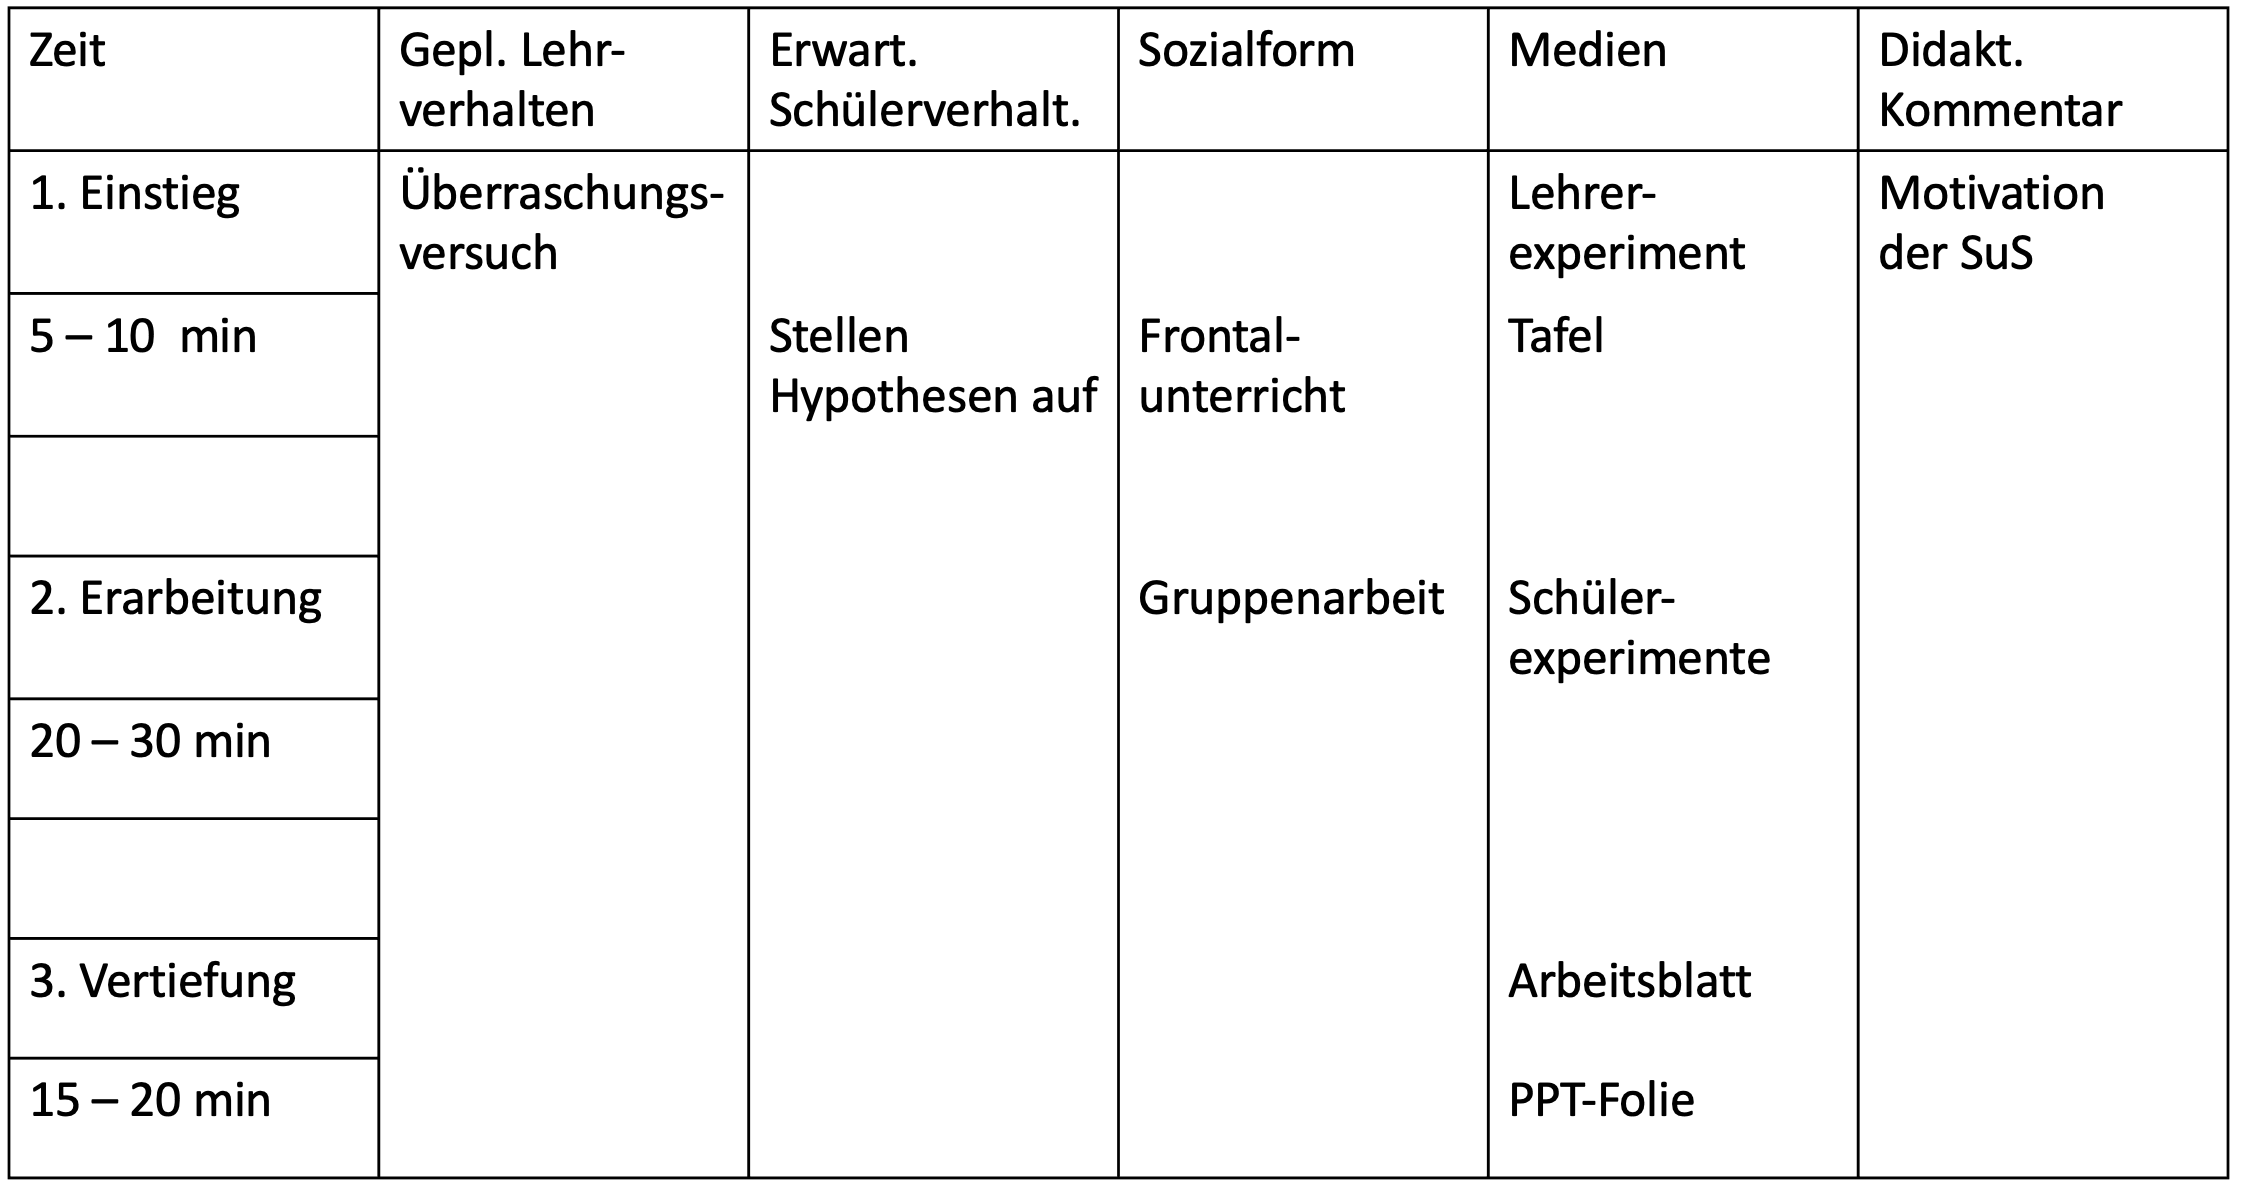
\includegraphics[scale=.2]{Unterrichtsskizze_02.png}
	\caption{Beispiel einer Unterrichtsskizze als Teil des Unterrichtsentwurfs}
	\label{fig:Unterrichtsskizze}
\end{figure}

\chapter{Experimentieren im Physikunterricht}\label{Experiment}

\section{Das Experiment als physikalisch-
                         erkenntnistheoretische Methode}

Die Physik beschreibt
\begin{itemize}
	\item
	in exakter Sprache (Logik, Mathematik, Fachterminologie)
	\item
	die Ph\"{a}nomene, die ,,unsere Welt'' (Kosmos, Natur,
	Alltag, Technik) grundlegend pr\"{a}gen.
\end{itemize}

Die Beschreibung ist nicht einfach enzyklop\"{a}disch-dokumentierend,
es wird vielmehr ein Gesamtsystem hergestellt, in dem
\begin{itemize}
	\item
	Ordnungsstrukturen und Hierarchien,
	\item
	Analogien und Modellvorstellungen,
	\item
	Ursachen und Wirkungen (Kausalit\"{a}t),
	\item
	Idealisierungen und Anwendungen
\end{itemize}
aufgezeigt werden.

Diese Ph\"{a}nomene nehmen Menschen mittels der Sinnesorgane wahr
\begin{itemize}
	\item
	zum Teil unmittelbar,
	\item
	zum Teil durch bewusste gezielte Herstellung von bestimmten
	Rahmenbedingungen im Experiment.
\end{itemize}

Der Erkenntnisgewinn der Physik vollzieht sich dabei in einem
Wechselspiel von
\begin{itemize}
	\item
	Experimentalphysik: Sie hat die Aufgabe, auf
	empirisch-induktivem Wege ausgehend von den Ph\"{a}nomenen
	Gesetzm\"{a}{\ss}igkeiten zu erschlie{\ss}en \\ und
	\item
	Theoretischer Physik:
	Hier werden auf logisch-deduktivem Wege die Gesetzm\"{a}{\ss}igkeiten
	auf ihre Geschlossenheit hin \"{u}berpr\"{u}ft, zusammengef\"{u}hrt und
	Folgerungen (f\"{u}r die Wirklichkeit) gezogen.
\end{itemize}

Die Physik ist also eine exakte empirische Naturwissenschaft.
Das Experimentieren ist unmittelbarer Bestandteil ihres Wesens.

\subsection{Kennzeichen von Experimenten}

Experimente m\"{u}ssen bei Durchf\"{u}hrung
\begin{itemize}
	\item
	zu anderen Zeiten (Wiederholung)
	\item
	an anderen Orten, bei anderen Ausrichtungen,
	\item
	bei Benutzung anderer Materialien, Ger\"{a}te,
	\item
	unter der Regie anderer Experimentatoren
\end{itemize}
zu identischen Ergebnissen f\"{u}hren
(wenn nicht diese Parameter unmittelbare Bestandteile der
Experimentieranordnung sind).

\bip
{ \bf
Experimentieren im Unterricht er\"{o}ffnet also zun\"{a}chst die
Einsicht in eine grundlegende Arbeitsweise der Physik und
damit der Naturwissenschaften \"{u}berhaupt.
}

\bip\bip
\section{Das Experiment als unterrichtlich-lerntheoretische
                                          Methode}

Unabh\"{a}ngig von der erkenntnistheoretischen Funktion dient das
Experimentieren im Physikunterricht
--- je nach konkreter Umsetzung ---
einer ganzen Reihe von \"{u}bergeordneten Lernzielen:

\begin{itemize}
	\item
	Schulung der Sinnesorgane (Beobachten,\dots)
	\item
	Artikulation der Beobachtungsergebnisse (Protokollierung,
	Sprachliche Beschreibung),
	\item
	Kognitive Entwicklung (Kausales Denken, Abstraktionsf\"{a}higkeit,
	                                Objektivit\"{a}t,\dots)
	\item
	Ausdauer, Geduld, Sorgfalt,
	\item
	Handwerklich-technische Kenntnisse
	(Werkstoffe, Ger\"{a}te, Sicherheitsvorkehrungen,\dots)
	\item
	Handwerklich-technische (Finger-)Fertigkeiten
	(Schrauben, L\"{o}ten, Regeln,\dots)
	\item
	Soziale Entwicklung (besonders bei Gruppenexperimenten).
	\item
	Affektive Dimension: Interesse, Abbau von \"{A}ngsten,
	Aha-  oder Erfolgserlebnisse.
\end{itemize}

oder Unterrichtsprinzipien

\begin{itemize}
	\item
	Handlungsorientierung, Selbstt\"{a}tigkeit (Sch\"{u}leraktivit\"{a}t).
	\item
	Unmittelbarkeit ,,Mit den eigenen Augen sehen!''
	\item
	Anschauung: Alle Sinne werden angesprochen.
	\item
	Alltagsn\"{a}he
	\item
	Wissenschaftsorientierung
\end{itemize}

\bip\bip
\section{Klassifikation von Unterrichtsexperimenten}
Experimente (synonym: Versuche) im Unterricht k\"{o}nnen
klassifiziert werden hinsichtlich verschiedenster Kategorien.

\subsection{Erkenntnistheoretische Funktion}
\begin{itemize}
	\item
	Erarbeitungsexperiment: Induktiv (Ph\"{a}nomen $\to$ Gesetz)
	\item
	Best\"{a}tigungsexperiment: Deduktive Methode (Gesetz $\to$ Ph\"{a}nomen)
	\item
	Gedankenexperiment: Ist das Gesetz in sich schl\"{u}ssig?
	\item
	Messung einer Natur-, Material- oder Ger\"{a}tekonstante.
	\item
	Modellexperiment: Um einen experimentell nicht oder nur schwer
	zug\"{a}nglichen Sachverhalt besser verstehen zu k\"{o}nnen,
	wird das Experiment an einem Modell durchgef\"{u}hrt:
	Bsp.: Maxwell'sche Geschwindigkeitsverteilung.
	\item
	Simulationsexperiment: (Die Wirklichkeit wird vorget\"{a}uscht,
	im Mittelpunkt stehen die Beobachtung und Auswertung).
	\item
	Historisches Experiment.
	\item
	Spielexperiment: Leistung meines K\"{o}rpers beim Treppensteigen.
	Astronomie-Modellspiele, Der Schwerpunkt beim Hochsprung,\dots
\end{itemize}

\subsection{Zeitliche Einordnung in einer Unterrichtseinheit}

\begin{itemize}
	\item
	Motivation oder Einstieg: Weckung eines kognitiven Konflikts ($\to$ Schülervorstellungen, \cref{Schuelervorstellungen})
	oder Show-Effekt.
	\item
	Problemstellung: Ein Experiment wirft ein Problem auf.
	\item
	L\"{o}sung: Erarbeitung (einer Gesetzm\"{a}{\ss}igkeit),
	Klassische Funktion des Experiments.
	
	\item
	Wiederholung, Festigung: Das Experiment wird wiederholt.
	
	\item
	\"{U}bertragung, Integration: Das Experiment wird --- unter ver\"{a}nderten
	Bedingungen bzw.\ Fragestellungen durchgef\"{u}hrt.
%	\item
%	\"{U}bung: %?!
\end{itemize}

\subsection{Intensit\"{a}t und Art der Auswertung}
\begin{itemize}
	\item
	Alternativ oder
	Qualitativ oder Quantitativ (Vgl.\ Elementarisierung).
	\item
	Messreihe, Diagramm.
	\item
	Anzeige, analog-digital, Computererfassung und Weiterverarbeitung.
\end{itemize}

\subsection{Art der Repr\"{a}sentation}
\begin{itemize}
	\item
	Reine Beobachtung eines Ph\"{a}nomens.
	\item
	(Frei-)Handversuch.
	\item
	Durchsichtige/Einsichtige Anordnung.
	\item
	Hoher Ger\"{a}teAufwand (Begriff der BlackBox).
	\item
	Computereinsatz.
\end{itemize}

\subsection{Experimentierort}
Physiksaal --- Klassenzimmer --- Pausenhof --- Sporthalle
 --- Sch\"{u}ler-Zuhause --- Natur/Umwelt (Wandertag, Klassenfahrt) --- vorbereitet als Video --- Simulationsexperimentierumgebungen.

\subsection{Experimentator}
\begin{itemize}
	\item
	Lehrer-Demonstrationsexperiment:
	Die Gr\"{u}nde daf\"{u}r sind vor allem pragmatischer Natur:
	
	\begin{itemize}
		\item Mangelnde Sicherheit f\"{u}r die Sch\"{u}ler oder die Ger\"{a}te
		\item Spontaneit\"{a}t (\"{U}berraschung) beispielsweise bei Freihandversuch oder innerhalb der
		Motivationsphase.
		\item Einheitliche Darbietung f\"{u}r alle Sch\"{u}ler
		(z.B.\ vor Leistungserhebung),
		\item Didaktisch oder fachlich versierte Darbietung durch den ,,Experten''
		\item Sch\"{u}ler\"{u}berforderung  hinsichtlich Kenntnissen, Eingew\"{o}hnung,
		Komplexit\"{a}t, Fertigkeiten
		\item Zeitknappheit ($\gets$ Lehrplan)
		\item Zu geringe Ger\"{a}te- bzw.\ Arbeitsplatzausstattung
		\item Disziplinprobleme
	\end{itemize}

	Lehrerdemonstrationsexperimente sind Bestandteil des eher
	darbietenden Unterrichts.
	
	\item
	Sch\"{u}ler-Demonstrationsexperiment
	Z.B.\ im Rahmen eines Sch\"{u}lerreferats.
	
	\item
	Sch\"{u}ler-Einzelexperiment:
	Schwierig ist die (ungelernte) spontane Beherrschung simultaner
	Arbeitsabl\"{a}ufe (Einstellen, in Gang setzen, ablesen,\dots),
	\item
	Sch\"{u}ler-Gemeinschaftsexperiment:
	Mischform, beispielsweise im Sch\"{u}lerkreis, Projektunterricht,
	soziale Erfahrungen (Lehrer und Ssch\"{u}ler handeln gemeinsam).
	\item
	Sch\"{u}ler-Gruppenexperiment: Siehe unten!
	\item
	Dritte (Im Film, Besichtigung,\dots).
\end{itemize}

\subsection{Sch\"{u}lerexperimente in Gruppenarbeit}

Vergleiche auch dazu die \"{U}berlegungen zum Begriff der
Gruppenarbeit als Sozialform.

\begin{itemize}
	\item
	Gruppengr\"{o}{\ss}e: 2 -- 6 Personen, mit oder ohne Lehrer.
	
	\item
	Rahmen: Einfache Experimente, evtl.\ Freihandexperimente,
	einfaches sicheres Ger\"{a}t und Material.
	\item
	Arbeitsauftrag:
	\begin{itemize}
		\item
		Parallel identisch (arbeitsgleich).
		Es k\"{o}nnen beispielsweise Mittelwerte gebildet werden.
		Der Lehrer kann gut steuern, beispielsweise bei typischen Fehlern.
		\item
		Parallel abwechselnd:
		Beispielsweise bei Ger\"{a}te- oder Arbeitsplatzmangel
		\item
		Parallel erg\"{a}nzend (arbeitsteilig):
		Die Sch\"{u}ler f\"{u}hren Experimente zum gleichen Themenkreis mit
		gleichen oder verschiedenen Auftr\"{a}gen durch;
		Ergebnisse f\"{u}hren zu einer gemeinsamen Probleml\"{o}sung
		(Richtung Projektarbeit).
		\item
		Frei (Experimentalfreiarbeit):
		Eine sehr reizvolle (Wagenschein'sche) Idealform, hoch motivierend.
		Kann z.B.\ in Neigungsgruppen, Helfergruppen oder
		Freizeitgruppen organisiert werden.
	
	\end{itemize}
	
	\item
	Eine gewisse Steuerung ist im Allgemeinen notwendig.
	Sie wird beispielsweise durch ein Arbeitsblatt oder eine
	aufgelegte Folie gew\"{a}hrleistet.
	Ein umfangreiches Programm kann so schneller absolviert werden.
	
	
	\begin{itemize}
		\item
		Der Lehrer oder Betreuer wird entlastet, er kann sich
		einzelnen Gruppen zuwenden.
		\item
		Themenstellung, evtl.\ Datum, Name, Klasse.
		\item
		Die Versuchsanordnung (ikonisch oder symbolisch)
		mit Beschriftungen.
		\item
		Die Art der Parameter, wie werden sie eingestellt?
		\item
		Mehr oder weniger genaue (kleinschrittige) Arbeitsanweisungen
		f\"{u}r die durchzuf\"{u}hrenden Versuche.
		\item
		Tabellen oder Koordinatensysteme f\"{u}r die Auswertung.
		\item
		L\"{u}ckentexte f\"{u}r die Ergebnisfixierung.
	
	\end{itemize}
	
	\item
	St\"{a}ndig wiederkehrende T\"{a}tigkeiten k\"{o}nnen separat einge\"{u}bt werden.
	Umgang mit Schaltungen allgemein, Befestigungstechnik,
	Bedienung von Messger\"{a}ten oder Netzger\"{a}ten, Bunsenbrenner.
	Im Laufe der Zeit sollten Sch\"{u}ler zunehmend selbst\"{a}ndig werden.
	
	\item
	Vorbereitende T\"{a}tigkeiten (Abzwicken von Dr\"{a}hten,
	Knoten von Schn\"{u}ren o.\"{a}., Entwirren von Kabelgeflechten)
	halten auf, sind aber u.U.\ auch f\"{u}r sich lehrreich.
	\item
	Materialien (m\"{o}glichst abgez\"{a}hlt, evtl.\ abgeteilt in Beh\"{a}ltern)
	werden bereitgestellt
	(Auf das Mitbringen von Gegenst\"{a}nden von Zuhause kann man sich u.U.\
	nicht verlassen).
	\item
	Innerhalb einer Gruppe k\"{o}nnen Funktionen vereinbart werden:
	Materialholer, Durchf\"{u}hrer, Protokollf\"{u}hrer, Berichterstatter.
	\item
	Der Arbeitsplatz sollte von \"{u}berfl\"{u}ssigen Gegenst\"{a}nden (B\"{u}chern,
	Schultaschen, Essen, Getr\"{a}nken) frei sein.
	Es gen\"{u}gen im Allgemeinen die Versuchsmaterialien und Schreibzeug.
\end{itemize}
	
Besonderheiten in der Stunde:
\begin{itemize}
	\item
	Das Experimentieren in Gruppenarbeit hat seinen Platz innerhalb der
	Erarbeitungsphasen der einzelnen Artikulationsschemata.
	Andere Phasen (Einstieg, Problemfrage, Fixierung,\dots)
	erfolgen gegebenenfalls im Klassenverband.
	\item
	Der Wechsel zwischen den Experimentiert\"{a}tigkeiten und
	Klassengespr\"{a}ch (Arbeitsauftr\"{a}ge, Erkl\"{a}rungen, Korrekturen)
	sollte eigentlich vermieden werden,
	er muss aber einge\"{u}bt werden.
\end{itemize}

\bip\bip
\section{Allgemeine Hinweise}
\begin{itemize}

	\item
	Versuchsanordnung
	\begin{itemize}
		\item
		Bewegungsabl\"{a}ufe, Input-Output-Vorg\"{a}nge, Lichtstrahlen
		sollten von links nach rechts bzw.\ von oben nach unten
		gerichtet sein.
		
		\item
		Die Versuchsanordnung sollte \"{u}bersichtlich sein.
		Dazu dienen zus\"{a}tzliche Markierungen (Plus- bzw.\ Minuspol),
		farbige Aufkleber, farbige Experimentierleitungen.
		\item
		Messinstrumente sollten gut ablesbar sein.
		W\"{a}hle die Messbereiche einsichtig und zweckm\"{a}{\ss}ig!
	\end{itemize}
	
	\item
	Das Problem der Redlichkeit (,,Tricksen''):
	Der Versuchsaufbau oder die Durchf\"{u}hrung werden so
	manipuliert, dass im Nachhinein ein erw\"{u}nschtes Ergebnis
	eintritt (,,Bilderbuchmesswerte'').
	
	Ist das guter Physikuntericht?
	
	\begin{beisp}
	\begin{itemize}
		\item
		Die Fahrbahn wird geneigt, damit die Reibungskraft
		kompensiert wird.
		\item
		Der Gartenerde oder dem Leitungswasser wird Salz beigemischt,
		damit sie/es sich als leitf\"{a}hig herausstellt.
		\item
		Dem Wasser im Hoffmann'schen Zersetzungsapparat wird Salzs\"{a}ure
		beigegeben, damit die Elektrolyse deutlich eintritt.
		\item
		Der Nullpunktsschieber an einem Kraftmesser wird verstellt.
	\end{itemize}
	\end{beisp}
	
	\item
	Protokollierung eines Experiments
	(auf Arbeitsblatt, im Hefteintrag,\dots)
	\begin{itemize}
		\item
		Aufbau: Skizze, Schaltbild mit
		Beschriftung oder Texterl\"{a}uterung.
		\item
		Durchf\"{u}hrung:
		Welche Gr\"{o}{\ss}en werden vorgegeben, eingestellt, variiert?
		\item
		Beobachtung.
		Welche Gr\"{o}{\ss}en werden beobachtet bzw.\ gemessen?
		\item
		Erarbeitung des Ergebnisses: Abgeleitete Gr\"{o}{\ss}en,
		graphische Auftragung, G\"{u}ltigkeitsbereich.
		\item
		Deutung, induktiv gewonnenes Gesetz.
	\end{itemize}
	
	\item
	Sicherheit beim Experimentieren: %Siehe EXP! ??
\end{itemize}

\bip\bip
\section{Freihandexperimente}

Vor einigen Jahren noch wurde das eher bel\"{a}chelt. Gegenw\"{a}rtig erfreuen sie
sich als ,,urspr\"{u}ngliche Erfahrung von Natur und Technik'' einer rasanten
Beliebheitssteigerung. %:
%\begin{itemize}
%	\item Grundschule: Genetischer Sachunterricht.
%	\item Mittelschule: Schon immer stark der handlungsorientierte, lebensnah-praktische
%	Ansatz.
%	\item Gymnasium: Natur und Technik-Unterricht in der 5.\ Klasse:
%	\item Realschule: Am st\"{a}rksten eher traditionell.
%\end{itemize}
\mip
Begleitmaterialien aller Art.
\mip
\"{O}ffentlichkeit: Sachb\"{u}cher, selber experimentieren, Fernsehsendungen.
\mip
Es widerspricht geradezu diesem Begriff, wenn man ihn
mit hoher Genauigkeit definieren wollte.
\mip
Die Wortbestandteile ,,Frei'' und ,,Hand'' geben erste Anhaltspunkte.


Im folgenden wird der Versuch unternommen, anhand von
verschiedenen Gesichtspunkten den Begriff n\"{a}her einzugrenzen.

Allgemein wird man von einem Freihandexperiment um so eher sprechen
k\"{o}nnen, je mehr die folgenden Kriterien erf\"{u}llt sind.
\begin{itemize}
	\item
	{\bf Nicht-Standardisierung}
	FHEe sollten frei gestaltet sein, vielleicht auf eigenen Ideen
	des Experimentators beruhen.
	Der Einsatz vorgegebener Versuchsaufbauten, wie sie
	beispielsweise von Lehrmittelfirmen angeboten werden,
	widerspricht grunds\"{a}tzlich der Idee von FHEen.
	\item
	{\bf Kurze Zeitdauer}
	Die Durchf\"{u}hrung eines FHEs sollte nicht sehr viel Zeit
	(d.h.\ Sekunden bis wenige Minuten) in Anspruch nehmen.
	Sie zeigen {\it Ph\"{a}nomene} eher pr\"{a}gnant-qualitativ als
	umfassend-quantitativ.
	\mip
	Eine individuelle, eigene, evtl.\ gar k\"{u}nstlerische, Gestaltung
	geben dem Unterricht eine ganz andere Intensit\"{a}t.
	
	\item
	{\bf Gegenst\"{a}nde und Materialien}
	Sie sollten dem unmittelbaren Erfahrungsbereich der
	Sch\"{u}ler entstammen:
	\begin{quote}
		Spielzeug ($\to$ ,,Spielzeug-Physik''), Haushalt, Hobby,
		Basteln, Freizeit, Werkzeug.
	\end{quote}
	Auch aus der Physiksammlung k\"{o}nnen unter Umst\"{a}nden
	Alltagsgegenst\"{a}nde bereitgestellt werden wie
	\begin{quote}
		Kompass, Lupe, Magnete, Taschenlampe, Battereien, Kleinspannungsnetzger\"{a}t.
	\end{quote}
	
	\mip
	Es erfolgt im Allgemeinen kein oder ein sehr
	einfacher Versuchsaufbau.
	Man kann nicht definitiv ausschlie{\ss}en, dass
	Stativmaterial verwendet wird, eventuell kann man
	aber auch Befestigungen mit W\"{a}scheklammern,
	Buchbeschwerungen, Schraubstock oder \"{a}hnlichem w\"{a}hlen.
	
	\mip
	Kosten sollten eher gering sein (Engl.: Low budget experiments).
	
	\item
	{\bf Spontaneit\"{a}t} Mit der ,,freien Hand'' k\"{o}nnte bedeuten,
	dass ein FHE spontan, d.h.\ ohne jede Vorbereitung aus dem
	Unterrichtsgeschehen heraus durchgef\"{u}hrt werden.
	Dies setzt eine gut geordnete, vielleicht reichlich mit
	FHE-Gegenst\"{a}nden ausgestattete Physiksammlung voraus,
	die nat\"{u}rlich auch gepflegt werden muss.
	
	\mip
	Unter Umst\"{a}nden kann ein FHE auch umfangreiche Vorbereitung
	erfordern, die dann in der Bereitstellung von
	Material
	(Bsp.: Eisblock, Selbst gebauter Tripelspiegel,\dots)
	oder in der Ein\"{u}bung des ,,Hand''elns
	(Bsp.: Besenstielgleichgewicht) oder Austestung besteht.
	
	\item
	{\bf Bestimmte Unterrichtsprinzipien} werden bedient:
	\begin{itemize}
		\item
		Lebensn\"{a}he (Alltagsn\"{a}he).
		\item
		Handlungsorientierung (Selbstt\"{a}tigkeit, Sch\"{u}leraktivit\"{a}t).
		\item
		Anschauung.
		\item
		\"{A}sthetik.
		\end{itemize}
		
		\item
		{\bf Bestimmte Lernziele} r\"{u}cken in den Mittelpunkt
		\begin{itemize}
		\item
		Affektive Lernziele: Interesse, Freude, Begeisterung.
		\item
		Psychomotorische Lernziele (bei Sch\"{u}lerexperimenten):
		Hand-Fertigkeiten (Basteln, Bedienung einfacher Ger\"{a}te)
		\item
		Kognitive Lernziele: Kenntnis einfacher Ph\"{a}nomene (Wagenschein)
	\end{itemize}
\end{itemize}

\subsection{Andere Gesichtspunkte}
\begin{itemize}

	\item
	{\bf Unterrichtsphasen}
	\begin{itemize}
		\item
		Motivation:
		Kognitiver Konflikt (vgl.\ auch N\"{a}he zur Zauberei, Magie),
		Show-Effekt.
		\item
		Erarbeitung:
		Entscheidung: Schwimmt das Plastillinschiff? /
		Kommt die Zwirnrolle? \\
		Vergleich: Gewichstskraft von Styroporblock und Bleikugel \\
		Absch\"{a}tzung: Wie gro{\ss} ist die Schallgeschwindigkeit?
		(Startklappe beim Hundertmeterlauf)
		\item
		\"{U}bung, Festigung, Best\"{a}tigung:
		(Gilt bei einer optischen Abbildung
		$g = 2f$, so ist $B=G$ und $b = g = 2f$.)
		
		Vorzeigen eines (vielleicht zerlegten) technischen Ger\"{a}tes
		Trockenbatterie, Fahrraddynamo, Gl\"{u}hbirne,\dots)
		
		\item
		Hausaufgabe (Strohhalmtr\"{o}te).
	\end{itemize}
	
	\item
	{\bf Organisationsformen}
	Vertretungsstunden, Freiarbeit, F\"{a}cher\"{u}bergreifender Unterricht,
	Projektunterricht (Projekttag),
	au{\ss}erhalb der Schule (Kindergeburtstag, Zauberabend).
	
	\item
	{\bf Ort des Experimentierens}
	Da FHEe im Allgemeinen nicht gro{\ss}artige Versuchsaufbauten
	erfordern, k\"{o}nnen sie auch leichter an anderen Orten
	als dem Physiksaal durchgef\"{u}hrt werden.
	
	\begin{quote}
		Klassenzimmer, Zuhause, Schulhof, Turnhalle,
		Schwimmbad, Wandertag, Schulfahrt, Schul\-land\-heim.
	\end{quote}
	
	\item
	{\bf Sicherheit}
	Nat\"{u}rlich sind auch bei FHEen die
	einschl\"{a}gigen Sicherheitsgrunds\"{a}tze voll zu beachten.
	
	\mip
	Insbesondere bei Sch\"{u}lerexperimenten, die wom\"{o}glich zuhause
	durchgef\"{u}hrt werden, muss gegebenenfalls (per Hefteintrag)
	eine Ermahnung ausgeprochen werden:
	\begin{itemize}
		\item
		Experimentiere nicht mit der Netzspannung, sondern nur mit
		Haushaltsbatterien!
		\item
		Schaue nie mit Lupen, Fernrohren oder \"{a}hnlichen optischen
		Ger\"{a}ten in die Sonne!
		\item
		Experimente, die du in der Schule siehst, k\"{o}nnen sich
		gef\"{a}hrlich auswirken, wenn sie zuhause wiederholt werden.
		\item
		Beim \"{O}ffnen von Elektroger\"{a}ten muss der Netzstecker gezogen sein!
		\item
		Sei vorsichtig mit Laserpointern, starken Federn, spitzen
		Gegenst\"{a}nden!
		\item
		Beim Experimentieren soll nicht gegessen oder getrunken werden.
	\end{itemize}

\end{itemize}

\begin{uea}
	Beurteilen Sie: Handelt es sich hierbei um Freihandexperimente?
	\begin{enumerate}[label=\alph*.]
			\item
		Das Modell eines Ottomotors oder einer Dampfmaschine
		wird demonstriert.
		\item
		Das Bild eines Regenbogens oder eines gl\"{u}henden Lavaflusses
		wird gezeigt.
		\item
		Die Sch\"{u}ler betrachten ein St\"{u}ck Kork unter dem Mikroskop.
		\item
		Ein Wagen bewegt sich gleichf\"{o}rmig auf der Luftkissenfahrbahn.
		\item
		Ein Sch\"{u}ler schleppt eine mit Steinen beladene Tasche in den
		4.\ Stock des Schulhauses.
		\item
		Ein Bolzen wird mit dem speziellen Apparat gesprengt. 
	\end{enumerate}
\end{uea}

\subsection{Logistik}

\begin{itemize}
	\item Paradiesische Zust\"{a}nde im Physiksaal ---  anders als in der Wirklichkeit.
	\item Aufbewahrung.
	\item Kollegium.
	\item Wesentliche Dinge vielleicht in einer Art Koffer (Mit 100 Teilen 1000 Experimente).
\end{itemize}

\subsection{Nachteile}

Es entstehen unter Umst\"{a}nden falsche Vorstellungen davon,
was Physik als Wissenschaft leistet
(und damit: \dots Physiker als Wissenschaftler leisten).

Spannungsfeld: Rechenphysik --- Frei gestaltete Physik.

\chapter{Medien im Unterricht}\label{Medien}

\section{Grundlagen}
\subsection{Begriff}
Engerer (praktischer) Begriff (Fr\"{o}hlich, 1974): Medien sind
\begin{itemize}
\item
technische Unterrichtshilfen, die der Lehrer einsetzt oder
\item
Lernmittel f\"{u}r die Hand der Sch\"{u}ler.
\end{itemize}

Im weiteren Sinne k\"{o}nnte man als Medium all das bezeichnen, was der
Informations\"{u}bertragung und -bewahrung dient:
Die Luft als Tr\"{a}germedium
des Schalls und des Lichts, das gesprochene Wort \dots.

\subsection{Ziele beim Einsatz von Medien}
\begin{itemize}
\item
Informationsvermittlung und -bewahrung
\item
Veranschaulichung: ,,Ein Bild sagt mehr als tausend Worte'',
Modellger\"{a}te, Modellversuche
\item
Entlastung des Lehrers von Routine\-t\"{a}tigkeiten zugunsten einer
p\"{a}dagogischen T\"{a}tigkeit
\item
Lebensn\"{a}he
\item
Differenzierung im Klassenunterricht, Steuerung
im Gruppenunterricht
\item
Vielf\"{a}ltige Variation des Unterrichtsgeschehens
\end{itemize}

\subsection{\"{U}berblick \"{u}ber typische Medien}
\begin{itemize}
\item Analoge Tafeln aller Art:
	\begin{itemize}
	\item Wandtafel (Kreidetafel)
	\item Lehrtafeln (Landkarten, Tabellen (PSE, Isotopen\-karte))
	\item Pinnwand
	\item Magnet\-haft\-ta\-fel
	\end{itemize}

\item Derzeit übliche AV-Ausstattung in Schulen
	\begin{itemize}
		\item ortsfester PC oder Laptop
		\item Beamer oder großer Bildschirm
		\item Dokumentenkamera
		\item Soundanlage
		\item Bring your own Device (BYOD): Lehrkraft bringt eigenes Gerät (i. d. R. Tablet) mit ins Klassenzimmer und kann dieses über Kabel oder drahtlos auf den Beamer spiegeln
		\item immer häufiger: Smartboards
	\end{itemize}

\item Weitere Medien
	\begin{itemize}
		\item Tageslichtprojektor
		\item CD-Spieler
		\item Bluetooth-Box
	\end{itemize}
\item Digitale Lernplattformen
	\begin{itemize}
		\item ByCS/mebis
		\item Teams
	\end{itemize}

%\item
%Projektoren aller Art:
%\begin{itemize}
%\item
%Tageslichtprojektor (TLP oder OHP),
%\item
%Video-Anlage, Diaprojektor, Filmprojektor, Episkop sind angesichts der Pr\"{a}senz von Computertechnologie praktisch verdr\"{a}ngt. \end{itemize}
%\item
%Audio-Ger\"{a}te aller Art:
%\begin{itemize}
%\item
%CD-Player (Akustik, Schwebungen).
%\item
%Tonbandger\"{a}t, Kassettenrekorder, Plattenspieler, Radioger\"{a}t (Schulfunk) finden sich heute kaum noch in der Schulpraxis.
%\end{itemize}
\end{itemize}

\section{Analoges Medium: die Wandtafel}
\begin{itemize}
\item Mittelpunkt: Die Tafel ist auch heute oft noch das Medium, das im
Mittelpunkt des Unterrichts steht,
symbolisch entspricht dies der Anordnung der Tafel in
der Mitte der Stirnseite des Klassenzimmers.

\item Dynamik: Das Tafelbild wird w\"{a}hrend einer Stunde entwickelt
und spiegelt daher die Dynamik eines Unterrichts\-verlaufs wider.

\item Planung: Meist wird es mehr oder weniger genau --- eventuell
ma{\ss}st\"{a}blich --- geplant.
Es enth\"{a}lt dann in m\"{o}glichst pr\"{a}gnanten, klaren Formulierungen einen
auch f\"{u}r den Sch\"{u}ler-Hefteintrag geeigneten Lehrtext
und zugeh\"{o}rige Skizzen, Zeichnungen oder Diagramme.

\item Spontaneit\"{a}t: Es kann aber auch spontan entwickelt werden
(Nebenrechnungen, Skizzen, Kurzerkl\"{a}rungen, Messwerte,\dots).
\end{itemize}

\bip
Hinweise zur Arbeits\-technik  an der Wandtafel:
\begin{itemize}
\item
Die Tafel sollte mit einem sauberen Lappen gewischt und dann
trocken sein.
\item
Achte auf gute Sichtverh\"{a}ltnisse: Beleuchtung der Tafel
m\"{o}glichst von vorne oben, Unterbindung von Reflexionslicht.
\item
Achte bei der Planung auf Eigenschaften der Tafel:
Gr\"{o}{\ss}e der Teiltafeln, Klappm\"{o}glichkeiten, Skalierung der K\"{a}stchen,
Befestigungsm\"{o}glichkeiten (Haken, Stative, Magnetclips)
Korrektur nach Trockenwischen, Annahme von Farbkreide.
\item
Soll die Tafel (grunds\"{a}tzlich) bez\"{u}glich verschiedener
Funktionen unterteilt werden: Konzepttafel, Nebenrechnungen,
Hefteintrag,\dots

\item
Spreche nicht zur Tafel! Stehe seitlich zur Schreibhand!
Quietschende Kreide sollte durchgebrochen werden.
\item
Achte auf den Zeitbedarf!
Das Tempo beim Tafelschreiben ist von selbst eher sch\"{u}lergem\"{a}{\ss}.
\item
Zeichnungen:
\begin{itemize}
\item
Beim Zeichnen von Kurven ist die Richtung von oben nach
unten g\"{u}nstiger!
\item
Die Hand sollte ---  unverkrampft --- in etwa senkrecht
zur momentanen Strichrichtung ausgerichtet sein.
\item
Arbeite m\"{o}glichst mit Hilfspunkten und/oder Symmetrien.
\item
Dr\"{u}cke Zeichenwerkzeuge immer in der N\"{a}he des aktuellen
Zeichnens an!
\item
Bei perspektivischen Darstellungen ist \"{U}bung (evtl.\ vorher
auf dem Papier) von Vorteil.
Entwickle die Darstellung bez\"{u}glich der Richtung senkrecht zur
Tafel ,,in die Tafel hinein'' (wegen der Verdeckungsrelationen)!
\mip
\"{U}bung: Zeichne einen Hufeisenmagneten, eine Spule
mit Andeutung der Windungsrichtungen, einen Quader (W\"{u}rfel),
eine Kugel.
\end{itemize}
\item
Falsches (Beispiele f\"{u}r typische Fehler) sollte als solches
kenntlich sein.
\end{itemize}

Spezielle Hinweise f\"{u}r Mathematik und Physik:
\begin{itemize}
\item
Der Kreidezirkel sollte in der N\"{a}he der Saugn\"{a}pfe
festgehalten werden.
Der Kreismittelpunkt muss vor dem Kreiszeichnen markiert werden
(Es gibt keinen Einstichpunkt).
\item
Beim Zeichnen von geometrischen Figuren oder Graphen
(Messwerte, Funktionsgraphen) arbeite man mit Hilfspunkten oder
Symmetrien! Werden Punkte eines Graphen mit $+$ statt $\times$ markiert,
so sind sie nach der Fertigstellung des Graphen leichter
erkennbar.
\item
Bei einem drei-dimensionalen  Koordinatensystem sollte die
zur Tafelebene senkrechte Achse nach vorne gezeichnet sein.
Dann wird sie nicht von Objekten im Quadranten der anderen beiden
Achsen verdeckt.
\item
Verwendung von ,,Icons'':
Auge, Mikroskop, Motor,\dots

\item
Verwendung von Symbolen: Schaltbilder von el.\ Schaltungen,
Befestigungen.
\end{itemize}

\section{Digitale Medien}
\subsection{Grundlagen: das SAMR-Modell}
\begin{figure}
	\centering
	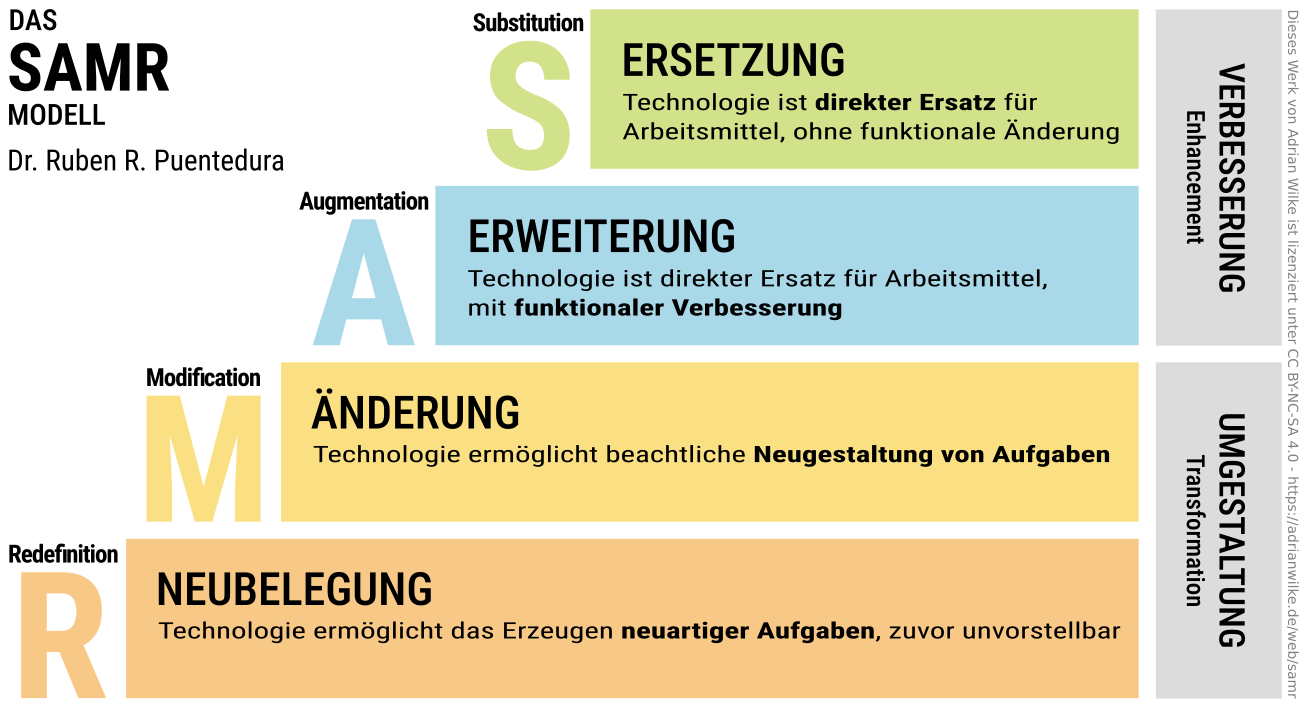
\includegraphics[width=.9\textwidth]{SAMR-Puentedura-deutsch.png}
	\caption{Das SAMR-Modell nach Puentedura}\label{fig:samr}
\end{figure}

Digitale Medien\footnote{Wir können hier nur einen knappen Einblick in spezifische Aspekte geben. Darüber hinaus verweisen wir auf die Veranstaltungen \emph{Lehren und Lernen mit und über digitale Medien} bei Dr. Seyferth-Zapf sowie \emph{Erstellung videobasierter LearningBits} aus unserem Kanon.} ergänzen den Einsatz analoger Medien sinnvoll und verdrängen diese teilweise bereits. Einen theoretischen Rahmen bildet das in \cref{fig:samr} illustrierte SAMR-Modell nach Dr. Ruben R. Puentedura, das die Integration von Technologie im Unterricht in vier Stufen beschreibt:
\begin{enumerate}
	\bitem{Substitution (Ersetzung)} Technologie ersetzt herkömmliche Werkzeuge, ohne grundlegende Änderungen am Unterrichtsprozess.
	\bitem{Augmentation (Erweiterung)} Technologie ersetzt herkömmliche Werkzeuge und bietet funktionale Verbesserungen.
	\bitem{Modification (Modifikation)} Der Einsatz von Technologie führt zu einer Umgestaltung der Lernaktivitäten.
	\bitem{Redefinition (Neudefinition)} Technologie ermöglicht völlig neue Lernformen, die ohne sie nicht möglich wären.
\end{enumerate}

\begin{beisp2}
	\begin{enumerate}
		\item Ein gedrucktes Arbeitsblatt wird durch ein digitales Dokument ersetzt.
		\item Das digitale Dokument enthält interaktive Elemente wie Links oder Kommentare.
		\item Lernende bearbeiten Projekte kollaborativ in Echtzeit über Online-Plattformen.
		\item Lernende erstellen Videos oder interaktive Präsentationen, um komplexe Konzepte zu vermitteln und weltweit zu teilen.
	\end{enumerate}
\end{beisp2}

Das Modell dient als Leitfaden, um den Einsatz von Technologie im Unterricht zu reflektieren und gezielt zu verbessern.

\subsection{Das Tablet als Tafel}
Tablets mit digitalen Stiften werden heute häufig für Tafelanschriebe verwendet. Dabei verwendet man eine Notizen-App wie Goodnotes oder das an vielen Schulen eingesetzte Microsoft OneNote. Der Tablet-Bildschirm wird auf den Beamer oder großen Bildschirm gespiegelt.

\mip
Grundlegend gelten dieselben Argumente wie für die Entwicklung eines Hefteintrags an der Kreidetafel, die Verwendung eines Tablets hat jedoch folgende \textbf{Vorteile} (=Augmentation):
\begin{itemize}
	\item Der Lehrer schaut zur Klasse.
	\item Das Geschriebene ist konserviert und kann 	ausgewertet, archiviert oder wiederverwendet (Wiederholung) werden. Entsprechende Apps erlauben den Export als PDF, sodass der Hefteintrag der Klasse digital zur Verfügung gestellt werden kann.
	\item Beinahe unendliche Kapazit\"{a}t. Die \say{Tafel} muss nicht gewischt werden.
	\item Beliebige Vielfalt bei den Vorlagen: Kariertes Papier, Koordinatensystem, Leertabelle, L\"{u}ckentext.
	\item Bilder können eingefügt und direkt beschriftet werden.
	\item
	Die Farbgebung ist einfacher.
	Die Zuordnung hell/dunkel bzgl.\ des Sch\"{u}lerhefteintrags stimmt
	(dunkel auf der Folie $\Rightarrow$ dunkel im Heft).
	\item Direkter Zugriff auf digitale Ressourcen wie Bilder, Animationen, Simulationen, Filme, \dots ohne Umschalten.
	\item Arbeisblätter können gemeinsam ausgefüllt werden.
\end{itemize}

Es gibt jedoch auch \textbf{Nachteile:}
\begin{itemize}
	\item Reizüberflutung der Schüler durch Übertechnisierung
	\item Tun des Lehrers nicht so gut erkennbar, nur Textentstehung, erschwert Nachahmung
	\bitem{Warnung} Man neigt im Digitalen zur Vorwegnahme, z. B. durch vorgefertigte Präsentationen. Dies kann den Konstruktionsprozess der Schüler behindern.
\end{itemize}

\subsection{Das Smartboard}
Ein Smartboard ist eine digitale Tafel, die Eigenschaften von Kreidetafel und Tablet auf sich vereint: Mit dem Finger oder mit digitalen Stiften kann auf ihrer Oberfläche geschrieben werden. Zudem können weitere Inhalte (z. B. Graphiken) eingebunden werden.

\begin{itemize}
	\item Aufgrund der Ähnlichkeit zur Kreidetafel gelten dieselben Warnhinweise wie für diese analog.
	\item Der Umgang mit Smartboard-Systemen ist häufig auch für Digital Natives nicht intuitiv und muss geübt werden. Ein \say{Kampf mit der Technik} ist eine der wesentlichsten Unterrichtsstörungen.
	\item In unserem Klassenzimmer \say{Luki} ist ein Smartboard verbaut, an dem Ihr gerne üben könnt.
\end{itemize} 

\subsection{Die Dokumentenkamera}
Eine Dokumentenkamera ist ein digitales Präsentationsgerät, das gedruckte oder physische Materialien in Echtzeit auf eine Projektionsfläche oder einen Bildschirm überträgt. Sie ermöglicht es Lehrkräften, Bücher, Arbeitsblätter oder Objekte visuell zu präsentieren und zu vergrößern, wodurch detaillierte Erklärungen vor einer größeren Gruppe möglich werden. Zudem kann sie oft mit anderen Geräten wie Computern oder interaktiven Whiteboards verbunden werden, um das gezeigte Material digital zu speichern oder weiterzubearbeiten.

\mip
Ihr Einsatz eignet sich besonders dann, wenn \dots
\begin{itemize}
	\item analoge Schülerarbeiten der Klasse gezeigt werden sollen, z. B. bei der Besprechung der Hausaufgabe oder der Bearbeitung eines Arbeitsblattes.
	\item die feinmechanische Vorgehensweise relevant ist, z. B. beim Eintragen von Messwerten in Diagramme.
	\item der Umgang mit Instrumenten gezeigt wird, z. B. die Einstellung des Messbereichs und das korrekte Ablesen der Messdaten bei Analogmultimetern.
\end{itemize}

\subsection{Der Tageslichtprojektor}
Heutzutage handelt es sich eher um ein Relikt, eine Vorstufe zu den vorgenannten Medien. Dennoch ist er nützlich zur Projektion mancher Experimente:

\begin{itemize}
	\item
	Mit dem TLP steht grunds\"{a}tzlich eine intensive
	Lichtquelle zur Verf\"{u}gung.
	\item
	Der TLP kann als Projektionslampe zum Schattenwerfen dienen:
	Kreisbewegung wird als harmonische Schwingung gesehen.
	Schatten einer Kerzenflamme.
	\item
	Anzeigeger\"{a}te mit transparenter Skala (Messinstrumente, Kompass)
	\item
	Licht-Schatten-Ph\"{a}nomene
	\item
	Mechanisch dynamische Vorg\"{a}nge: Sto{\ss}en, Ablenken,
	Stahlnagel-Elektromagnet, Oersted-Versuch.
	\item
	Farbmischung (Subtraktiv bei farbigen Folien)
\end{itemize}

\subsection{Aspekte des Einsatzes von Computern im Physikunterricht}

\begin{itemize}
	\bitem{Als klassisches AV-Medium} Bilder, Filme, Animationen, Simulationen, PowerPoint-Präsentationen, \dots
	\bitem{Schulung von Medienkompetenz} Als schulart- und fächerübergreifendes Bildungs- und Erziehungsziel ist Medienbildung und digitale Bildung auch im Physikunterricht relevant.
	\begin{itemize}
		\item Bedienung physikspezifischer Programme: Experimentierumgebungen, Datenerhebung und -auswertung (PhET, Excel, GeoGebra, \dots)
		\item Bewertung von Internetquellen hinsichtlich ihrer Glaubwürdigkeit
		\item Recherchemöglichkeiten im Internet
		\item Gestaltung ansprechender Präsentationen, z. B. mit PowerPoint
	\end{itemize}
	\bitem{Schulung von Programmierfähigkeiten} In der Zusammenarbeit mit Mathematik und Informatik ist algorithmisches Denken auch in der Physik wichtig. Programmierfähigkeiten lassen sich bspw. bei der Umsetzung der Methode der kleinen Schritte schulen.
	\bitem{Computer als Unterrichtsgegenstand} Physikalische Grundlagen heutiger und zukünftiger Computertechnologie
	\bitem{Digitale Messwerterfassung}
	\begin{itemize}
		\item Eine Vielzahl von digitalen Sensoren (Bewegung, Lichtschranken, Kraft, Druck, Schall, Stromstärke, Spannung, Temperatur, Magnetfeld, \dots) lassen sich über USB oder drahtlos mit dem PC verbinden und die Daten auslesen.
		\item Verbreitete Systeme: \textbf{CASSY, Phywe, Vernier}
		\item Zugriff auf Primär- und Sekundärdaten (z. B. Ort und Geschwindigkeit durch Integration über Daten des Beschleunigungssensors) mittels geeigneter Software
		\item Direkte Darstellung der erhobenen Daten in Tabellen oder Diagrammen
		\item Speicherung der Messergebnisse
		\item Vorteile:
			\begin{itemize}
				\item Schnelle, bequeme Bedienbarkeit $\to$ Zeitersparnis.
				\item Vielseitigkeit: Vergleiche oben.
				\item \"{U}bersichtliche Aufbewahrung $\to$ Platzersparnis.
				\item Standardisierung,
				\item Blackbox-Prinzip: Der wesentliche Gehalt eines Experiments kann besser herausgearbeitet werden.
				\item Verfügbarkeit und Portabilität der Daten: Ergebnisse eines Lehrerexperiments können Schülern zur weiteren Analyse zur Verfügung gestellt werden.
			\end{itemize}
		\item Nachteile:
			\begin{itemize}
				\item Die Unmittelbarkeit der messenden Erfassung von physikalischen Ph\"{a}nomenen geht verloren.
				\item Handwerkliche Fertigkeiten werden in den Hintergrund gedr\"{a}ngt.
				\item Zunehmende Abh\"{a}ngigkeit von ausgefeilten Technologien.
				\item Kosten f\"{u}r Neuanschaffungen. Eigentlich sind Messwerterfassungssysteme vergleichsweise billig.
				\item Blackbox-Prinzip: Messprinzip kann verschleiert werden.
			\end{itemize}
	\end{itemize}
\end{itemize}

\section{K\"{u}nstliche Intelligenz \`{a} la ChatGPT --- speziell im Physikunterricht}

ChatGPT und verwandte Angebote zur Nutzung k\"{u}nstlicher Intelligenz sind erst k\"{u}rzlich allgemein zug\"{a}glich geworden, erfreuen sich aber bereits allergr\"{o}{\ss}ter Beliebtheit insbesondere bei Sch\"{u}lerinnen und Sch\"{u}lern, sowie Studenten. Die Entwicklung der k\"{u}nstlichen Intelligenz steht noch am Anfang, sodass damit zu rechnen ist, dass sich die zur Verf\"{u}gung stehenden M\"{o}glichkeiten und die Qualit\"{a}t der Ergebnisse stetig weiterentwickeln werden. Auf eine Darstellung, was ChatGPT ist und wie man es benutzt, wird hier verzichtet. Vielmehr sollen hier Ideen skizziert werden, auf welche Weise ChatGPT gewinnbringend im Physikunterricht eingesetzt werden kann.

\begin{enumerate}
\item \textbf{Generieren von Inhalten:} ChatGPT kann mit gro{\ss}er Leichtigkeit Texte und eine Vielzahl von Grafiken erzeugen. 
	\begin{beisp} 
	\say{\emph{Erstelle mir eine kurze Zusammenfassung zum Film \say{The Fast and the Furious}, die ich in einer dreimin\"{u}tigen Pr\"{a}sentation in der Schule verwenden kann, im Sprachstil von Letty Ortiz!}}
	\end{beisp}

\item \textbf{Study-buddy:} Sch\"{u}ler k\"{o}nnen  mit ChatGPT interaktiv und im eigenen Tempo \"{U}bungsfragen durchgehen und Rechenaufgaben l\"{o}sen. Physikalische Konzepte k\"{o}nnen durch ChatGPT verst\"{a}ndlich erkl\"{a}rt werden und im Dialog mit ChatGPT erlernt werden. Im Gegensatz zu Google ist KI in der Lage, einen Dialog mit dem Bedienenden zu f\"{u}hren, auf Fragen zu antworten, auf Nachfrage zu pr\"{a}zisieren, Beispiele zu liefern, Gegenbeispiele zu liefern usw.. ChatGPT kann somit als Gespr\"{a}chspartner in simulierten Diskussionen \"{u}ber physikalische Themen dienen. 
	\begin{beisp}
	\glqq\emph{Nenne mir ein Experiment, mit dem nachgewiesen wird, dass die Ladung des Elektrons wirklich negativ ist!}\grqq,  analysiere die generierte Antwort kritisch, und stelle Folgefragen, beispielsweise \glqq\emph{Wird durch dieses Experiment wirklich das Vorzeichen der Ladung ermittelt?}\grqq.  
	\end{beisp}

\item \textbf{Ideengeber bei Hausaufgaben und Projekten:} Sch\"{u}ler k\"{o}nnen ChatGPT nutzen, um Unterst\"{u}tzung bei Hausaufgaben, Projektideen oder der Recherche nach Informationen zu physikalischen Themen zu erhalten. 
	\begin{beisp} 
	\glqq\emph{Nenne mir drei Experimente zum Nachweis des Strahlencharakters von Licht f\"{u} den Physikunterricht der 8. Klasse!}\grqq
	\end{beisp}

\item \textbf{Begutachtung von schriftlichen Arbeiten und Vorbereitung auf Pr\"{u}fungen:} Sch"{u}ler k\"{o}nnen ChatGPT nutzen, um sich auf Pr\"{u}fungen vorzubereiten, indem sie Fragen stellen, Erkl\"{a}rungen wiederholen und gezielte R\"{u}ckmeldungen zu ihren Antworten erhalten. ChatGPT kann als virtueller Gutachter verwendet werden, um eigene Textentw\"{u}rfe zu begutachten. 

	\begin{beisp} 
	Ziehen Sie eine pdf-Datei mit einer selbsterstellten Ausarbeitung oder auch eine Grafik in den Eingabeprompt und bitten Sie um eine Zusammenfassung oder eine Analyse bzw. Bewertung!
	\end{beisp}
	
	
\item \textbf{Unterst\"{u}tzung f\"{u}r Lehrkr\"{a}fte:} Lehrer k\"{o}nnen ChatGPT als Hilfsmittel bei der Unterrichtsvorbereitung einsetzen, z.B. zum Erstellen von \"{U}bungsaufgaben, zur schnellen Recherche oder als Inspirationsquelle f\"{o}r neue Unterrichtsideen. 
	\begin{beisp2}
	\begin{itemize}
	\item {\glqq}\emph{Gib die erforderlichen Lernvoraussetzungen, Lernziele und eingesetzte Medien in einer Unterrichtsstunde zum Fadenstrahlrohr an.}{\grqq} 
	\item {\glqq}\emph{Gestalte eine sch\"{u}lerzentrierte Unterrichtseinheit zum Thema elektrische Influenz in der Mittelstufe. W\"{a}hle ein Artikulationsschema des entdeckenden Unterrichts. Gehe explizit auf Vorwissen und Lernziele ein und verdeutliche, wie durch die Ma{\ss}nahmen dieser Unterrichtseinheit die gesetzten Lernziele erreicht werden k\"{o}nnen.}{\grqq} 
	\end{itemize}
	\end{beisp2}
\end{enumerate}
\bip

ChatGPT erm\"{o}glicht  nicht nur effizientes und kreatives Arbeiten, ebenso kann ChatGPT  den Physikunterricht bereichern, indem es personalisierte Lernm\"{o}glichkeiten bietet  und den Zugang zu komplexen Inhalten vereinfacht. Durch die Verwendung von ChatGPT wird das selbstgesteuerte Lernen stark gef\"{o}rdert und eine Bef\"{a}higung zum zum kritischen und ausgiebigen Dialog angestrebt.
\mip
Es ist jedoch darauf zu achten, dass der Einsatz von ChatGPT bewusst gesteuert wird, um sicherzustellen, dass es als Erg\"{a}nzung und nicht als Ersatz f\"{u}r den direkten Unterricht und die zwischenmenschliche Interaktion dient. Beim Generieren von Inhalten wird die Eigenleistung der Lernenden im kreativen Recherche- und Schreibprozess umgangen. Lehrkr\"{a}fte m\"{u}ssen sich mit den M\"{o}glichkeiten durch ChatGPT vertraut machen und klare Regeln zu dessen Anwendung aufstellen.
\mip
Letztlich muss gewarnt werden, dass ChatGPT gelegentlich zum {\glqq}Halluzinieren{\grqq} neigt, d.h. dass es frei erfundene Antworten erzeugt. Output von ChatGPT sollte daher niemals  ungepr\"{u}ft \"{u}bernommen werden. 

\section{Schriftliche Medien --- f\"{u}r die Hand der Sch\"{u}ler}
\subsection{Das Schulbuch}

\subsection{Arbeitsbl\"{a}tter und -hefte}
\begin{itemize}
\item
Selbstgestaltet --- vorgefertigt.
\item
Inhalte k\"{o}nnen korrekt und auf den Punkt gebracht
dargestellt werden.
\item
Gestaltung individuell: Tabellen, Diagramme, Bilder, Skizzen.
\item
M\"{o}gliche Sch\"{u}leraktivit\"{a}ten (Begleitet auf der Folie):
\begin{itemize}
\item
Erg\"{a}nzung: L\"{u}ckentexte, Tabellen, Zeichnungen.
\item
Farbige Gestaltung: Texte markieren, Skizzen f\"{a}rben,
           Zeichnungs\-tei\-le kennzeichnen.
\item
Beschriften von Zeichnungen, Diagrammen.
\item
Grafische Gestaltung: Unterstreichen, Einrahmen, Schraffieren.
\end{itemize}

\item
\"{O}konomie: Zeitersparnis im Unterricht, in der Vorbereitung.
\item
Arbeitsblatt-Verwaltung durch den Lehrer:
Heute mit PC m\"{o}glich und vielf\"{a}ltig.

\item
Probleme:
\begin{itemize}
\item
,,Zettelwirtschaft'' bei Sch\"{u}lern (G\"{u}nstig: Nummerierung, Datumsangabe (Kieserblock).
\item
Eine beim Lehrer hervorgerufene ,,Stoffabarbeitungs-Philosophie''
korrespondiert mit einem Minimal-Aufwand an Vorbereitung.
Im Unterricht ruft dies einen Eindruck von Eint\"{o}nigkeit hervor.
(Es gibt Verlage, die genau diese Art von Lehrermentalit\"{a}t bedienen:
,,Da brauchen Sie nur noch in der Fr\"{u}h schnell kopieren''.)
\end{itemize}
\end{itemize}

\subsection{Das Sch\"{u}lerheft}

Praktische Hinweise f\"{u}r Zeichnungen:
\begin{itemize}
\item
Beim Zeichnen von Kurven/Graphen setze den Handballen in der
N\"{a}he auf und ziehe den Strich in Schreibrichtung!
Eventuell sollte vorher das Heft gedreht werden.

\item
Zeichnungen sollten nach M\"{o}glichkeit mit
Bleistift angefertigt werden,
da dann das Radieren m\"{o}glich ist.
(Auch wegen Verdeckungen muss manchmal radiert werden.)
\end{itemize}


\chapter{Schulprofile}

\section{Das Profil des  Gymnasiums}\label{Gymnasium} 

Das Gymnasium ist eine weiterf\"{u}hrende Schulform in Deutschland, die auf eine umfassende, wissenschaftsorientierte Allgemeinbildung abzielt und mit dem Abitur abgeschlossen wird. Das Abitur berechtigt zum Studium an Universit\"{a}ten und Hochschulen und ist der h\"{o}chste allgemeinbildende Schulabschluss in Deutschland.

Wesentliche Merkmale des Gymnasiums sind:

\begin{itemize}
	\item \textbf{Bildungsangebot:} Das Gymnasium bietet eine breite und vertiefte Allgemeinbildung in einer Vielzahl von F\"{a}chern. Dazu geh\"{o}ren neben den Kernf\"{a}chern Deutsch, Mathematik und Fremdsprachen auch Naturwissenschaften, Gesellschaftswissenschaften, Kunst, Musik und Sport. Der Unterricht ist darauf ausgerichtet, die Sch\"{u}ler zu selbstst\"{a}ndigem Denken und wissenschaftlichem Arbeiten zu bef\"{a}higen.
	
	\item \textbf{Fremdsprachenunterricht:} Ein besonderes Merkmal des Gymnasiums ist der intensive Fremdsprachenunterricht. In der Regel beginnen die Sch\"{u}ler mit einer ersten Fremdsprache ab der 5. Klasse und einer zweiten Fremdsprache ab der 6. oder 7. Klasse. Oft besteht die M\"{o}glichkeit, eine dritte Fremdsprache oder ein bilinguales Angebot zu w\"{a}hlen.
	
	\item \textbf{Oberstufe und Abitur:} Die gymnasiale Oberstufe (Klassen 10 bis 12 oder 11 bis 13, je nach Bundesland) ist modular aufgebaut und erm\"{o}glicht den Sch\"{u}lern eine gewisse F\"{a}cherwahl nach ihren Interessen und Begabungen. Die Sch\"{u}ler bereiten sich auf das Abitur vor, das aus einer Kombination von schriftlichen und m\"{u}ndlichen Pr\"{u}fungen besteht. Das Abitur qualifiziert f\"{u}r das Studium an Universit\"{a}ten und Fachhochschulen.
	
	\item \textbf{Wissenschaftsorientierung:} Der Unterricht am Gymnasium ist stark auf wissenschaftliche Arbeitsweisen ausgerichtet. Dies umfasst analytisches Denken, methodisches Arbeiten und die F\"{a}higkeit zur kritischen Reflexion. Projekte, Facharbeiten und Experimente f\"{o}rdern die forschungsorientierte Herangehensweise an Themen.
	
	\item \textbf{Breite Wahlm\"{o}glichkeiten:} Das Gymnasium bietet eine Vielzahl von Wahlpflichtf\"{a}chern und Profilen an, die es den Sch\"{u}lern erm\"{o}glichen, Schwerpunkte nach ihren Interessen zu setzen. Diese Profile k\"{o}nnen in Bereichen wie Naturwissenschaften, Sprachen, Musik oder Kunst liegen.
	
	\item \textbf{Pers\"{o}nlichkeitsentwicklung und Sozialkompetenz:} Neben der fachlichen Ausbildung legt das Gymnasium Wert auf die Entwicklung sozialer Kompetenzen und der Pers\"{o}nlichkeitsbildung. Durch Klassenfahrten, Sch\"{u}leraustausche, AGs und Projekte werden Teamf\"{a}higkeit, Verantwortungsbewusstsein und Eigeninitiative gef\"{a}rdert.
	
	\item \textbf{Studien- und Berufsorientierung:} Das Gymnasium bereitet die Sch\"{u}ler nicht nur auf das Abitur, sondern auch auf das sp\"{a}tere Studium oder Berufsleben vor. Berufs- und Studienberatungen, Praktika und Informationsveranstaltungen unterst\"{u}tzen die Sch\"{u}ler bei ihrer beruflichen Orientierung.

\end{itemize} 

Das Gymnasium bietet somit eine anspruchsvolle und vielseitige Ausbildung, die auf ein breites Spektrum an akademischen und beruflichen M\"{o}glichkeiten vorbereitet. Es legt den Grundstein f\"{u}r ein weiterf\"{u}hrendes Studium und f\"{o}rdert die umfassende Entwicklung der Sch\"{u}ler in intellektueller, sozialer und pers\"{o}nlicher Hinsicht.


\bip\bip
\section{Das Profil der Realschule}\label{Realschule} 

Die Realschule ist eine weiterf\"{u}hrende Schulform in Deutschland, die nach der Grundschule beginnt und in der Regel nach der 10. Klasse mit einem mittleren Schulabschluss (Realschulabschluss) endet. Sie bietet eine praxisnahe und zugleich theoretisch fundierte Allgemeinbildung, die auf verschiedene Bildungs- und Berufsperspektiven vorbereitet.

Wesentliche Merkmale der Realschule sind:

\begin{itemize}
	
	\item \textbf{Bildungsangebot:} Die Realschule vermittelt eine breite Allgemeinbildung in den Kernf{\ss}chern wie Deutsch, Mathematik und Fremdsprachen sowie in den Naturwissenschaften, Gesellschaftswissenschaften und F\"{a}chern wie Kunst, Musik und Sport. Neben theoretischem Wissen werden auch praktische F\"{a}higkeiten vermittelt, oft in Form von Projekten oder Praxisphasen.
	
	\item \textbf{Berufsorientierung:} Ein zentrales Ziel der Realschule ist die Vorbereitung auf den Einstieg in die Berufswelt. Dies geschieht durch eine enge Verzahnung von Theorie und Praxis, z.B. durch Betriebspraktika, Berufsberatung und Projekte mit Unternehmen. Die Realschule legt gro{\ss}en Wert auf die F\"{o}rderung von Schl\"{u}sselkompetenzen, die f\"{u}r das Berufsleben wichtig sind.
	
	\item \textbf{Differenzierung und F\"{o}rderung:} Die Realschule bietet verschiedene Wahlpflichtf\"{a}cher an, die es den Sch\"{u}lern erm\"{o}glichen, nach ihren Interessen und Begabungen Schwerpunkte zu setzen, z.B. in den Bereichen Wirtschaft, Technik oder Sprachen. Zudem gibt es gezielte F\"{o}rderangebote f\"{u}r Sch\"{u}ler, die Unterst\"{u}tzung in bestimmten F\"{a}chern ben\"{o}tigen.
	
	\item \textbf{Abschluss und Perspektiven:} Der Abschluss an der Realschule qualifiziert f\"{u}r den Eintritt in eine duale Ausbildung oder in weiterf\"{u}hrende Schulen wie Fachoberschulen, Berufskollegs oder das Gymnasium (unter bestimmten Voraussetzungen). Der Realschulabschluss ist anerkannt und bietet eine solide Grundlage f\"{u}r vielf\"{a}ltige berufliche und akademische Wege.
	
	\item \textbf{Soziale und Pers\"{o}nlichkeitsentwicklung:} Neben der fachlichen Ausbildung f\"{o}rdert die Realschule die soziale Kompetenz und Pers\"{o}nlichkeitsentwicklung der Sch\"{u}ler. Durch Klassenfahrten, Projekte und au{\ss}erunterrichtliche Aktivit\"{a}ten werden Teamf\"{a}higkeit, Verantwortungsbewusstsein und Selbstst\"{a}ndigkeit gest\"{a}rkt.
	
	Die Realschule bietet somit eine ausgewogene Mischung aus praxisorientierter Bildung und theoretischem Wissen, die sowohl f\"{u}r den direkten Einstieg in die Berufswelt als auch f\"{u}r weiterf\"{u}hrende Bildungswege geeignet ist.
\end{itemize}

%\section{Das Profil der Mittelschule}\label{Mittelschule} 
%Die Mittelschule ist
%eine weiterf\"{u}hrende Schule, sie umfasst die Jahrgangsstufen
%5 -- 9 (10).
%
%Grunds\"{a}tzliches Spannungsfeld:
%\begin{quote}
%	Wissenschaftsorientierung   \q $\ctr$\q
%	Person-Welt-Orientierung
%\end{quote}
%
%\mip
%\"{U}bergeordnete Erziehungsziele sind (Vgl.\ Blatt 1):
%
%\begin{itemize}
%	\item
%	Grundlegende Allgemeinbildung: Kenntnisse, Ganzheitliche Weltsicht.
%	\item
%	Verantwortung in der Welt: Kultur, Werte, politische Bildung.
%	\item
%	Lebensbew\"{a}ltigung: Ern\"{a}hrung, Pers\"{o}nliche Entwicklung,
%	Freizeit, Medien, Verkehr.
%	\item
%	Orientierung f\"{u}r das Arbeitsleben: Kenntnisse f\"{u}r das
%	Berufsleben, Hilfe bei der Berufswahl.
%\end{itemize}
%
%Folgende Abschl\"{u}sse sind m\"{o}glich:
%\begin{itemize}
%	\item
%	Erfolgreicher Hauptschulabschluss
%	($\to$ Ausbildung in Handwerk, Industrie, Dienstleistung)
%	\item
%	Qualifizierender Hauptschulabschluss
%	($\to$ Meister, Techniker, mittlerer nichttechnischer
%	Verwaltungsdienst)
%	\item
%	Mittlerer Schulabschluss ($\to$ FOS, BAS, Studium)
%\end{itemize}
%
%----------
%----------
%\mip
%\pph{\"{A}u{\ss}ere Form des Lehrplans} VERALTET!
%
%Die drei Ebenen:
%\begin{itemize}
%	\item
%	Grundlagen und Leitlinien.
%	\item
%	\"{U}bergeordnete Unterrichts und Erziehungsaufgaben
%	\begin{quote}
%		Fachbezogen --- Fach\"{u}bergreifend.
%	\end{quote}
%	\item
%	Einspaltige Fachlehrpl\"{a}ne.
%	\begin{itemize}
%		\item
%		Lernziele (vgl.\ auch S.\ 17) werden jeweils in
%		einer \"{U}berschrift (Zweistellige GliederungsNummer) beschrieben.
%		Die Lernziele sind nach didaktischen Schwerpunkten geordnet (S.\ 17)
%		\item
%		Es folgen die Lerninhalte ((Dreistellige GliederungsNummer)
%		\item
%		Die Einzelinhalte sind unter Spiegelstrichen aufgelistet.
%	\end{itemize}
%	\item
%	Es ist zu Beginn eines Schuljahres ein aktueller
%	Klassenlehrplan zu erstellen mit Ber\"{u}cksichtigung
%	\begin{itemize}
%		\item
%		von Absprachen und Querverweisen,
%		\item
%		des Schulbuchs, der Medienauswahl,
%		\item
%		Ortes der Schule,
%		\item
%		der Jahreszeitlichen Gegebenheiten.
%	\end{itemize}
%
%\end{itemize}
%
%Computereinsatz: S.\ 15, S.\ 50., S.\ 66.

\chapter{Literatur zur Physik und Didaktik}

\section{Empfohlene Literatur zur Vorlesung {\glqq}Grundlagen der Fachdidaktik{\grqq} der UBT}
\begin{itemize}
	\item \fullcite{KircherGirwidzHaussler3}
	\item \fullcite{LabuddeMetzger}
	\item \fullcite{Schecker}
	\item \fullcite{Wilhelm}
	\item \fullcite{JankMeyer}
	\item \fullcite{KircherSchneider}
	\item \fullcite{Boxer}
	\item \fullcite{JPMeyn}
\end{itemize}


\section{Zeitschriften}
\begin{itemize}
	\item %\fullcite{PhiuZ}
	Physik in unserer Zeit
	\item %\fullcite{PhuD}
	Physik und Didaktik
	\item %\fullcite{PdNPh}
	Praxis der Naturwissenschaften -- Physik
	\item %\fullcite{NiUPh}
	Naturwissenschaften im Unterricht -- Physik
	\item %\fullcite{PhBl}
	Physikalische Blätter
	\item %\fullcite{MNU}
	Der Mathematisch-Naturwissenschaftliche Unterricht
	\item %\fullcite{SpdW}
	Spektrum der Wissenschaft
\end{itemize}

% das hier waren alles uralte Schulbücher
%\section{Physik inhaltlich, Niveau Sekundarstufe I}
%\begin{itemize}
%	\item \fullcite{BornHubscherLochhaas}
%
%	\item \fullcite{DuitFries}
%	\item \fullcite{WiesnerOptikI}
%\end{itemize}



%Preiswerte Sammlung \"{u}ber alles Wissenswerte
%aus den Naturwissenschaften: \fullcite{MeyerSchmidt}
%
%\section{Physik inhaltlich, Niveau Sekundarstufe II}
%\fullcite{SahmWiller}
%\fullcite{Schlichting}
%
%Formelsammlung: \fullcite{HammerHammer}
%
%\section{Astronomie, Niveau Sekundarstufe II}
%\fullcite{Lermer}
%\fullcite{BeckmannEpperlein}
%\fullcite{Hasemann}
%\fullcite{Henkel}
%
%\section{Physik inhaltlich, Niveau Grundstudium}
%\fullcite{GerthsenVogel},
%\fullcite{AlonsoFinn}.
%
%Formelsammlung: \fullcite{Stoecker}.

%Lexikon: \fullcite{abcPhysik1}, \fullcite{abcPhysik2}.

\section{Fachdidaktik Physik}
\begin{itemize}
	\item \fullcite{KircherGirwidzHaussler1} (downloadbar unter \url{https://katalog.uni-bayreuth.de:443/TouchPoint/perma.do?q=35%3D%22(OCoLC)1220881218%22+IN+%5B2%5D&v=ubt&b=0&l=de})
	\item \fullcite{KircherGirwidzHaussler2} (downloadbar unter \url{https://katalog.uni-bayreuth.de:443/TouchPoint/perma.do?q=35%3D%22(OCoLC)1199763053%22+IN+%5B2%5D&v=ubt&b=0&l=de})
	\item \fullcite{KircherGirwidzHaussler3}
	\item \fullcite{KircherSchneider}
	\item \fullcite{DuitHausslerKircher}
	\item \fullcite{BleichrothDahnckeJung}
	\item \fullcite{Braun}
	\item \fullcite{WagenscheinPDP}
	\item \fullcite{LabuddeATP}
	\item \fullcite{LabuddeEWP}
	\item \fullcite{Muckenfuss}
	\item \fullcite{Ploeger}
%	\item \fullcite{WegeinderPhysikdidaktik1}
%	\item \fullcite{WegeinderPhysikdidaktik2}
%	\item \fullcite{WegeinderPhysikdidaktik3}
	\item \fullcite{WegeinderPhysikdidaktik4}
	\item \fullcite{Willer}
\end{itemize}


\section{Erziehungswissenschaften}
\begin{itemize}
	\item \fullcite{MeyerUMT}
	\item \fullcite{MeyerUMP}
	\item \fullcite{Koeck}
	\item \fullcite{Reble1}
	\item \fullcite{Reble2}
\end{itemize}



\section{Experimente --- Unterhaltsame Physik}
\begin{itemize}
	\item \fullcite{Lindenblatt}
	\item \fullcite{Aulas}
	\item \fullcite{Dussler}
%	\item \fullcite{ABD98}
	\item \fullcite{Berge}
	\item \fullcite{MelenkRunge}
	\item \fullcite{ZeierKW}
	\item \fullcite{KnoffHoff1}
	\item \fullcite{KnoffHoff2}
%	\item \fullcite{Wittmann1}
%	\item \fullcite{Wittmann2}
\end{itemize}


%\section{Schulb\"{u}cher Mittelschule}
%Es handelt sich um Schulb\"{u}cher (evtl.\ mit Kopiervorlagen oder
%Lehrerbegleitb\"{a}nden), die auf den Lehrplan (1997/98)
%bezogen sind.
%Als Beispiel sind jeweils nur die PCB-B\"{u}cher der 7.\ Jahrgangsstufe
%angegeben:
%\begin{itemize}
%\setlength{\itemsep}{0mm}
%\item Bayerischer Schulbuch-Verlag:
%       Natur entdecken \fullcite{Schurius7} \fullcite{Schurius7L}
%
%\item Cornelsen-Verlag: Natur und Technik \fullcite{Hiering7}
%\item Klett-Verlag: Urknall \fullcite{Litz7}
%\item Schroedel:
%       Natur plus \fullcite{ScharfSchulz7} \fullcite{ScharfSchulz7M}
%
%\item Westermann: Natur bewusst \fullcite{HausfeldSchulenberg7}
%                        \fullcite{HausfeldSchulenberg7K}
%                        \fullcite{HausfeldSchulenberg7L}
%\end{itemize}


\newgeometry{left=2.5cm, right=2.5cm, top=2.5cm, bottom=2.5cm} %ab jetzt wieder ohne Notizenrand
% Literaturverzeichnis
\printbibliography

\appendix
\chapter{Teilkompetenzen der KMK-Bildungsstandards}\label{A_kmk}
aus: ISB. Gute Aufgaben im Physikunterricht – erkennen – einsetzen – erstellen –. Kompetenzorientierter Unterricht am Gymnasium. München 2023.
\includepdf[pages=7]{ISB_Gute_Aufgaben_im_Physikunterricht}

\chapter{Verblisten für Operationalisierte Lernziele}\label{A_Verbliste}
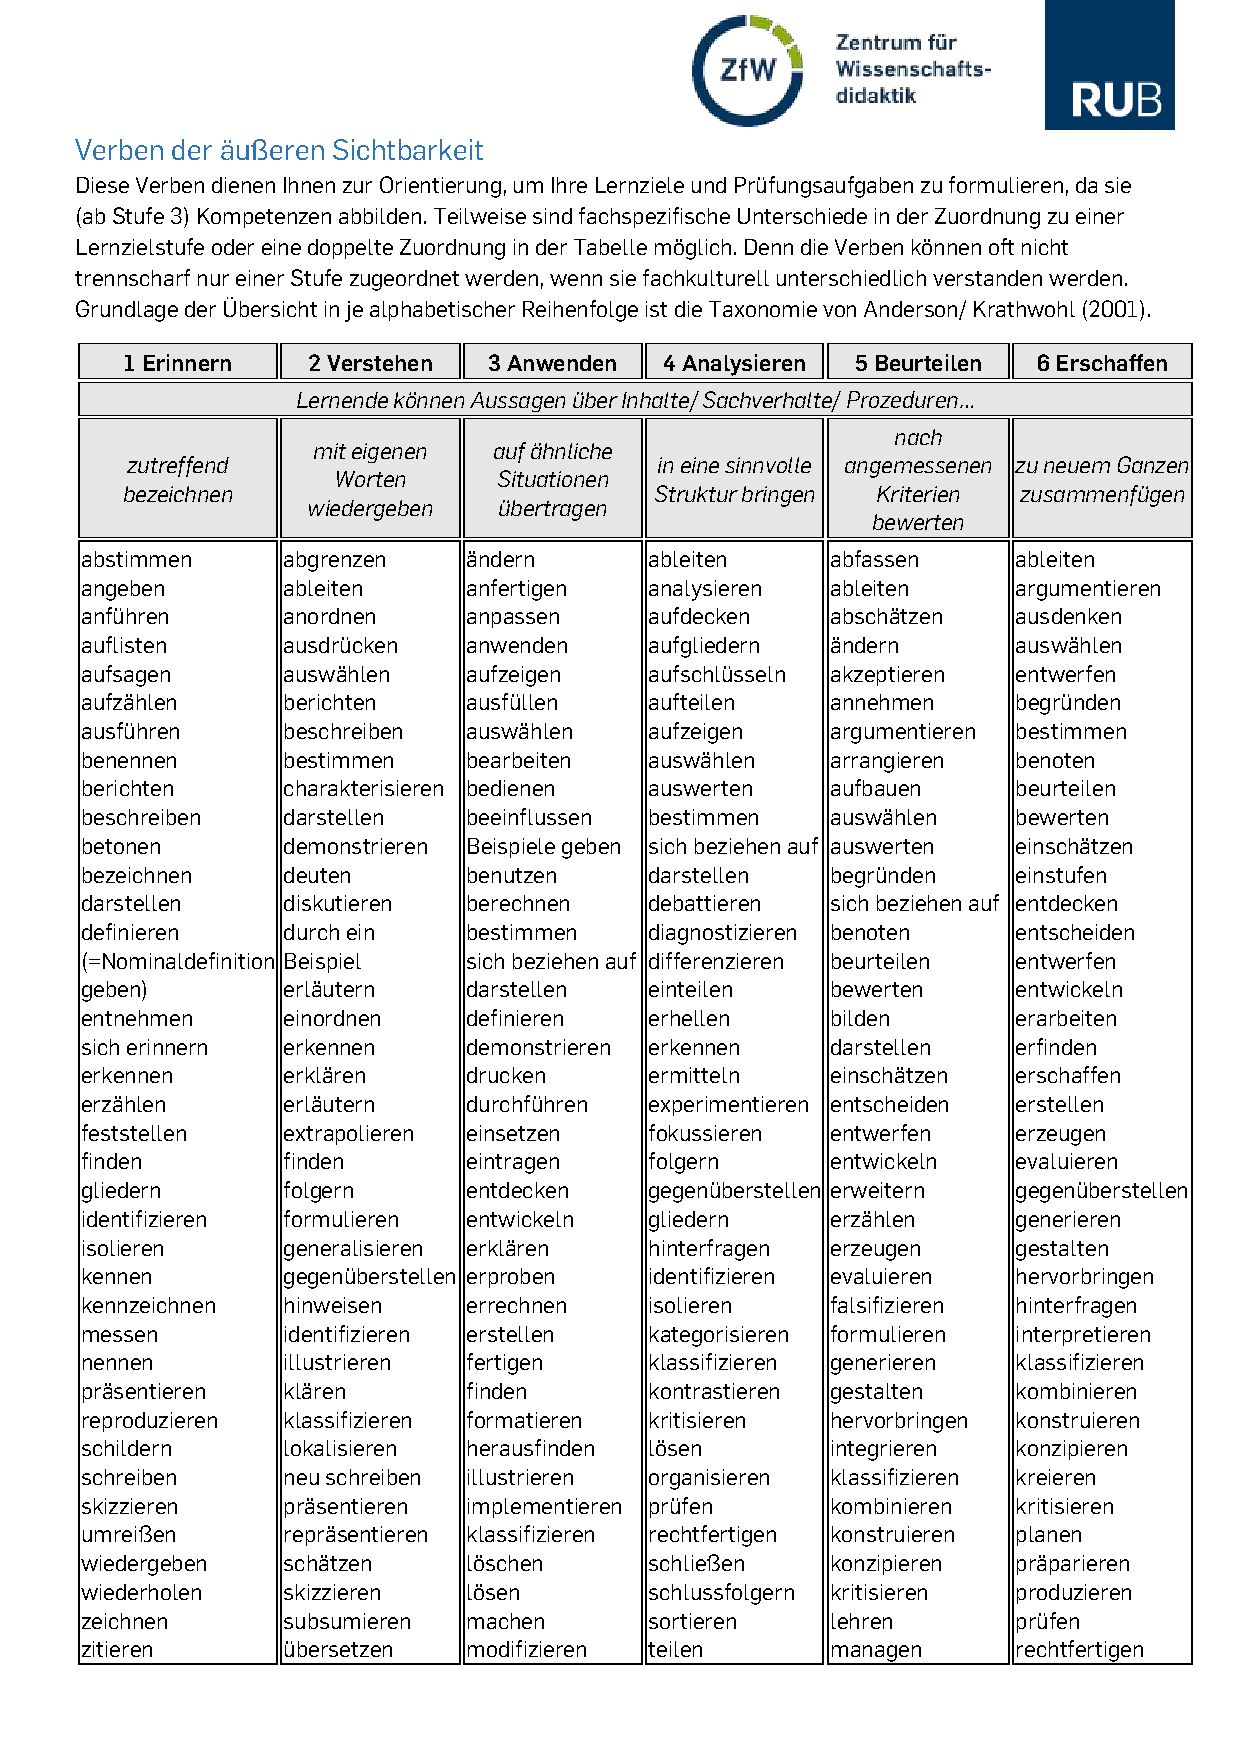
\includepdf[pages={1-2}]{Bilder/Verblisten_Kompetenz}

\chapter{Berliner Modell}\label{A_BerlinerModell}

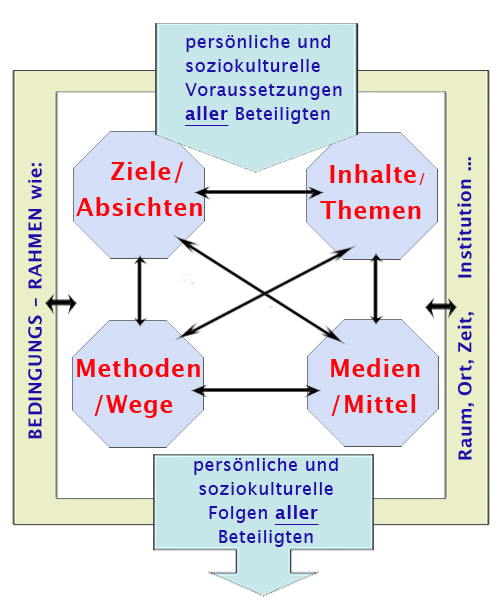
\includegraphics[width=10cm]{BerlinerModell1.jpg} \\
Bildquelle: \url{https://commons.wikimedia.org/wiki/File:BerlinerModell1.jpg}

\chapter{Weitere Artikulationsschemata}

\section{Grob-Phasen gem\"{a}{\ss} \textcite{DuitHausslerKircher}}
\begin{enumerate}
	\item {\bf Motivation} oder Einstiege
	\item {\bf Erarbeitung} Probleml\"{o}sung (beispielsweise im Experiment)
	\begin{enumerate}
	\item
	Planung des Experiments
	\item
	Durchf\"{u}hrung des Experiments
	\item
	Auswertung des Experiments
	\item
	R\"{u}ckblickende Er\"{o}rterung des Experiments
	\item
	Allgemeine Er\"{o}rterung
	\end{enumerate}
	\item {\bf Vertiefung} Integration, Behalten, Transfer.
\end{enumerate}

\section{\textcite{Ploeger}: Forschender Physikunterricht}
Konkret, anwendungsnah und auf den Punkt gebracht wird dieses Konzept in
\textcite{Ploeger} beschrieben.
Es finden sich dort auch viele Beispiele.
\begin{enumerate}
	\item {\bf Problemfrage}
	\item {\bf Vermutung}
	\item {\bf Versuchsplanung}
	\item {\bf Experiment}
	\item {\bf Auswertung}
\end{enumerate}
Der zentrale Unterschied zu Mothes ist die Sichtweise, aus der sie ihre Schemata formulieren. Während Mothes eher lehrerzentriert argumentiert, betont Plöger die aktive Beteiligung der Schüler an der Erarbeitung des Wissens.

\section{H.F.\ Bauer: Experimentalunterricht (1984)}
Das Grundschema des entdeckenden Unterrichts wird
hier spezialisiert-differenziert im Hinblick auf
das Experimentieren umgesetzt.

\mip Ziel des Unterrichts ist nicht Forschung an sich, sondern eine
Vertrautheit mit dem Forschen an sich.
	\begin{enumerate}
	\item {\bf Motivation}
	\item {\bf Problemherstellung}
	\item {\bf Meinungsbildung}
	\item {\bf Planen} und Konstruieren
	\item {\bf Laborieren --- Experimentieren}
	\item {\bf Schlie{\ss}en}
	\item {\bf Abstrahieren}
	\item {\bf Wissenssicherung durch Anwendung und \"{U}bung}
\end{enumerate}


\chapter{Beispiel einer didaktischen Analyse}\label{A_DidAna}

\end{document}